%%%%%%%%%%%%%%%%%%%%%%%%%%%%%%%%%%%%%%%%%%%%%%%%%%%%%%%%%%%%%%%%%%%%%%%%%%%%%%%%
%                                                                              %
% Copyright (C) 1998-2005 by MPI-CBS                                           %
%                                                                              %
% Max-Planck-Institute of Cognitive Neuroscience                               %
% PO Box 500 355, D-04303 Leipzig, Germany                                     %
%                                                                              %
% Phone +49 341 9940-00                                                        %
% Fax   +49 341 9940-113                                                       %
%                                                                              %
% EMail info@cbs.mpg.de                                                        %
% WWW   http://www.cbs.mpg.de                                                  %
%                                                                              %
% This software may be freely copied, modified, and redistributed provided     %
% that this copyright notice is preserved on all copies.                       %
%                                                                              %
% You may not distribute this software, in whole or in part, as part of any    %
% commercial product without the express consent of the author.                %
%                                                                              %
% There is no warranty or other guarantee of the fitness of this software      %
% for any purpose. It is provided solely "as is".                              %
%                                                                              %
%%%%%%%%%%%%%%%%%%%%%%%%%%%%%%%%%%%%%%%%%%%%%%%%%%%%%%%%%%%%%%%%%%%%%%%%%%%%%%%%

%%%%%%%%%%%
% Setting %
%%%%%%%%%%%

%%%%%%%%%%%%%%%%%%%%%%%%%%%%%%%%%%%%%%%%%%%%%%%%%%%%%%%%%
% Dissertation by Stefan Zysset and Claudia Danielmeier %
%%%%%%%%%%%%%%%%%%%%%%%%%%%%%%%%%%%%%%%%%%%%%%%%%%%%%%%%%

\documentclass[a4paper,11pt,twoside]{book}

\usepackage[english]{babel}     % english, or usepackage[ngerman]{babel} for german
\usepackage[ansinew]{inputenc}   % latin1 input encoding
\usepackage[T1]{fontenc}        % font encoding
\usepackage{apacite}            % citations style
\usepackage{graphicx}           % for including pictures
\usepackage{color}              % for color stuff
\usepackage{rotating}           % rotating tables, figures, ...
\usepackage{subfigure}          % for side by side pictures
\usepackage{longtable}          % multiple pages tables 
\usepackage{times}              % Adobe PostScript Fonts
\usepackage{mathptm}            % Adobe PostScript Fonts
\usepackage{courier}            % Adobe PostScript Fonts
\usepackage{exscale}            % misc packages
\usepackage{setspace}           % line distance
\usepackage{calc}               % linear measures
\usepackage{caption}            % adjust captions
\usepackage{multicol}           % text with multiple columns
\usepackage{booktabs}           % formatting command for tables
\usepackage{dcolumn}            % formatting command for tables
%\usepackage{parskip}           % free line between paragraphs and no indentation on the next line
\usepackage{fancyhdr}           % adjust footer and header
\usepackage{siunitx}
\usepackage[inner=4cm,
            outer=3cm,
            top=3cm,
            bottom=3cm,
            includeheadfoot]{geometry} % Seitenlayout bei zweiseitigen Dokumenten (book, ...)

\usepackage{german}
\usepackage{eurosym}

%%%%%%%%%%%%%%%%%%%%%%%%%%%%%%%%%
% new table and figure captions %
%%%%%%%%%%%%%%%%%%%%%%%%%%%%%%%%%

\renewcommand{\captionfont}{\small\itshape}
\renewcommand{\captionlabelfont}{\small}


%%%%%%%%%%%%%%%%%%%%
% more formattings %
%%%%%%%%%%%%%%%%%%%%

\singlespacing % bzw. \doublespacing, \singlespacing

%%%%%%%%%%%%%%%%%%%%%%%%%
% penalty customization %
%%%%%%%%%%%%%%%%%%%%%%%%%

% if a line of a paragraph is on the next page
\clubpenalty = 10000
\widowpenalty = 10000
\displaywidowpenalty = 10000

% if words overhanging
\tolerance = 500
\setlength{\emergencystretch}{2em} 

% paragraphs sehen aus wie subsubsubsections
%\titleformat{\paragraph}[hang]{\bf}{\thetitle\quad}{0pt}{}						
%\titlespacing{\paragraph}{0pt}{1em}{1em} 

% subparagraphs sehen aus wie vorher paragraphs
%\titleformat{\subparagraph}[runin]{\bf}{}{0.5em}{}
%\titlespacing{\subparagraph}{0pt}{1em}{1em}

%%%%%%%%%%%%%%%%%%%%%%%%%%%%%%%%%%%%%%%%%%%%%%%%%%
% clear header style on the last empty odd pages %
%%%%%%%%%%%%%%%%%%%%%%%%%%%%%%%%%%%%%%%%%%%%%%%%%%

\makeatletter
  \def\cleardoublepage{\clearpage\if@twoside \ifodd\c@page\else%
  \hbox{}%
  \thispagestyle{empty}%
  \newpage%
  \if@twocolumn\hbox{}\newpage\fi\fi\fi}
\makeatother

%%%%%%%%%%%%%%%
% hyphenation %
%%%%%%%%%%%%%%%

\hyphenation{mor-pho-syn-tax}

%%%%%%%%
% text %
%%%%%%%%

\begin{document}
\scrollmode

%%%%%%%%%
% title %
%%%%%%%%%

%\chapter{Titlepage}\label{titlepage}

\thispagestyle{empty}
\begin{titlepage}

%%%%%%%%%%%%%%%
% blaue Reihe %
%%%%%%%%%%%%%%%

\vspace*{3cm}

% Schmutztitel
\begin{center}
  \rule{14.5cm}{0.5mm}\\
  \vspace{0.5cm}
  \huge
  Title Title Title Title
  \rule{14.5cm}{0.5mm}
\end{center}

% Druckinfo
\clearpage
\thispagestyle{empty}
\vspace*{18cm}
\footnotesize{
ISBN 3-936816-XX-X
\vspace{1cm}

Druck: S\"achsisches Druck- und Verlagshaus Direct World, Dresden

\copyright \hspace*{1.5mm} 2005, Max Mustermann, Titelbild: \copyright \hspace*{1.5mm} 2005, XXX
}
\clearpage
\thispagestyle{empty}

%%%%%%%%%%%%%%%%%%%%
% Ende blaue Reihe %
%%%%%%%%%%%%%%%%%%%%

% Titelseite
\begin{center}
\normalsize
  {\huge Title Titel Titel Titel\\Title Titel Titel Titel Title Titel Titel Titel Title Titel Titel Titel}

  \vfill

  Der Fakult\"at für\\
  Biowissenschaften, Pharmazie und Psychologie\\
  der Universit\"at Leipzig\\
  eingereichte

  \vfill

  {\LARGE \textsc{Dissertation}}

  zur Erlangung des akademischen Grades

  doctor rerum naturalium\\
  Dr. rer. nat.

  \vfill

  vorgelegt\\
  von Dominic Portain\\
  geboren am 17. Juli 1985 in Ulm

\end{center}
\clearpage
\thispagestyle{empty}
\begin{center}
\normalsize

  \hspace{0cm}
  \vfill

  Dekan:\\
  Prof. Dr. XXX XXX

  Gutachter:\\
  Prof. Dr. XXX XXX\\
  Prof. Dr. PhD. XXX XXX\\
  Prof. Dr. XXX XXX

  \vfill

  Tag der Verteidigung: Leipzig, den \today

  \vfill

\end{center}
\end{titlepage}
\thispagestyle{empty}


%%%%%%%%%%
% Thanks %
%%%%%%%%%%

%\input{chapter/thanks}

%%%%%%%%%%%%%%%%%%%%%%%%%%%%%%%%%%%%%%%%%%%%%%%%%%%%%%%%%%%%%%%%%%%%%%%%%%%%%%%%%%%%%%%%
% Wenn du m�chtest, dass Vorspann, Hauptteil und Nachspann deines Dokuments seperat    %
% nummeriert werden, dann trenne diese Teile mittels \frontmatter, \mainmatter und     %
% \backmatter. Alles zwischen den ersten beiden bekommt (standardm�ssig) r�mische      %
% Ziffern, nach \mainmatter wird alphanumerisch gez�hlt (von Eins an), und \backmatter %
% z�hlt (standardm�ssig) weiter, das l�sst sich aber konfigurieren                     %
%%%%%%%%%%%%%%%%%%%%%%%%%%%%%%%%%%%%%%%%%%%%%%%%%%%%%%%%%%%%%%%%%%%%%%%%%%%%%%%%%%%%%%%%

\frontmatter

%%%%%%%%%%%%
% Contents %
%%%%%%%%%%%%

% header and footer
\pagestyle{fancy}

\fancypagestyle{plain}{%
\fancyhf{}   % clear all header and footer fields
\renewcommand{\headrulewidth}{0pt}
\renewcommand{\footrulewidth}{0pt}}

\renewcommand{\headrulewidth}{0pt}     % no head rule
\fancyhead{}                           % delete head
\fancyfoot{}                           % delete footer
\fancyhead[OR]{\thepage}               % page number
\fancyhead[OL]{\nouppercase\rightmark} % rightmark is the section
\fancyhead[ER]{\nouppercase\leftmark}  % leftmark is the capitel
\fancyhead[EL]{\thepage}               % page number

\clearpage
\cleardoublepage
\tableofcontents

\mainmatter


\chapter{Introduction}

\section{Neurobiological background}
\subsection{Exploration strategies of white matter tracts}
The human brain can be regarded as an information-processing system, processing and storing environmental stimuli in order to create meaningful actions. 
In a very simplified information-processing perspective, it can be reduced to two functional components: computational units in the grey matter and signal relays in the white matter.
Contrary to other common information-theoretical systems, there is no fundamental distinction between hardware and software in the brain.
Both structural elements (e.g., dendritic spines) and computational units (e.g., astroglial cells) are part of an inseparable information process.
The fact that anatomical features can't be clearly mapped to a functional role violates the naive reductionist approach, and puts cognitive science more in line with other fields that explore dynamical systems, such as physics, theoretical computer science or meteorology.
Although the exploration of anatomic features (e.g., the classification of cortical regions based on myeloarchitecture) led to several ground-breaking discoveries in psychology, these findings tend to serve as a base for more specialized studies, rather than creating a framework for understanding cognitive processes.

Most anatomical features offered a direct link between their structure and functional roles, providing a solid basis for functional research.
In the context of the human brain, there was one major exception: cerebral white matter, comprised of myelinated axons and glial cells.
The role of cerebral nerve fibers eluded scientific inquiry for centuries, mainly due to their microscopic structure and the unknown function of their end connection points.
The idea that they played a role in signal transmission (in the loosest sense) can be traced back as early as 1710 \cite{1.1.history}.
In the writings of Pourfoir de Petit, nerve fiber bundles were theorized to transmit animal spirits from the cortex to the medulla oblongata.
The complete motor transmission chain as known today, including the path from from the medulla to the extremities via the spinal cord, was discovered only 40 years later by Emanuel Swedenborg \cite{1.1.history}.
However, during the next 250 years, the exploration of the role of cerebral fiber tracts was stifled by the lack of a non-invasive, large-scale measurement method.

These circumstances abruptly changed in 1972 \cite{1.1.history}, when the discovery of the autoradiographic method allowed tracing the precise interneural connections with radioactive markers.
Radioactive tracing was very widely used to fill existing knowledge gaps in cognitive science, but one fundamental flaw has prevented its application in humans: not only is the tracer very invasive, but the subject needs to be killed and dissected in the course of the experiment.
This drawback has prevented the study of the role of human fiber bundles, and not all knowledge gaps could be filled with equivalent results from lab animals.

One of the most important set of fiber bundles that eluded autoradiographic study was the human language network.
Only with the advent of main-stream diffusion imaging \cite{1.1.firstDiffusion} in the mid-1980s, examinations of human fiber bundles in vivo started to be possible.
The analysis of the previously elusive language-related fiber bundles is still ongoing, while new methods in both acquisition and data processing proceed to advance.
But before I give an overview over the language network, some fundamentals need to be explained first.

\begin{figure}[h]
\begin{center}
\vspace{7mm}
\includegraphics[width=0.75\textwidth]{pics/1_1_myelin_sheath}
\caption{\label{1.1.neuron.illustrated} Illustration of an axonal fiber, wrapped in myelin layers. Adapted from Mosby's Medical Dictionary, 8th edition. \textcopyright 2009, Elsevier.}
\end{center}
\end{figure}

\subsection{The role of myelination}\label{1.1.myelin}
When regarding the brain from an information-theoretical perspective, it is important to consider that it is a self-optimizing structure with two important optimization constraints: the mechanism of myelination and limited space.

The importance of myelination becomes clear when regarding the mechanism of long-distance cerebral signal transmission.
Long-distance nerve fibers typically transmit signals in the form of electric fields.
This transmission process relies on the interplay of ion channels and electric currents.
Since the signal propagation is based on an activation cascade of ion channels, the transmitted signal is strictly binary in nature, is limited in bandwidth by a refractory period of $\approx 1ms$ and can only travel in one direction at a time.
The typical propagation speed of a nerve fiber is only $0.1\frac{m}{s}$, but can be increased by several magnitudes when enveloped by myelin layers.
Myelin layers, produced by myelinating sheath cells, reduce the amount of electrical current lost to the extracellular (usually liquid) environment.
This effect causes not only a higher propagation speed, but also an equally increased maximum signal bandwidth, since the refractory period stays constant.

Myelination causes not only positive aspects, but also creates a major drawback: it increases the volume of the nerve fiber drastically.
For an practical illustration, A-$\gamma$-fibers, responsible for relaying hot and cold sensations, have a diameter of \SI{3}{\um} and propagate signals at $15\frac{m}{s}$.
In comparison, A-$\beta$-fibers, responsible for sensing touch on the skin, have a diameter of \SI{10}{\um} and propagate signals with a speed of $50\frac{m}{s}$.
The cross section of this fiber class is 11 times bigger, although its effective bandwidth is only three times higher.
The volume requirements of myelination follow a law of diminishing returns: a single fiber with a high propagation speed requires more space than two fibers at half the speed, although the combined bandwidth is equivalent.

Since the brain is situated in an inflexible skull cavity, overall volume for the whole network (and, in effect, for every nerve fiber) is fundamentally volume-constrained.
Myelination is flexible and adaptive, so bandwidth can be increased by adding additional myelin layers to fibers in high demand.
Due to the volume constraints, this is only possible when neighboring fibers are reduced in diameter by the same volume.

This combination of constraints has apparently led to the prominent "'small-world"'' topology featured in every level of the central nervous system \cite{1.1.smallWorld}.
This type of network is characterized by a large number of very local connections; in fact, almost the majority (47.8\%) of all nodes are only connected to their nearest neighbors.
The small-world topology is a natural result of the trade-off that is created by minimizing the network distance between nodes while using the smallest amount of connections.
It is also responsible for one of the most convenient characteristics in cognitive science, the specialized brain region.
In a strongly local network, neural clusters in close proximity can share their information most effectively in closest network proximity.
And since neural clusters can choose to connect to other clusters most relevant to their task, this network proximity also becomes a functional proximity.
In a small-world-topology, this functional proximity becomes a spatial proximity.
Therefore, the optimal solution for information processing at any network level is to group neuronal clusters with similar tasks into a common spatial region.
As a result, the brain is highly structured into distinct functional regions, and regions in close proximity usually exchange signals with each other.

The combination of volume constraints and myelination properties creates another trade-off in one of the most fundamental tasks of the brain: learning.
Learning, on a neural level, always requires some form of change.
This change can occur within the neuron, for example by tweaking the input weights of established connections.
In other cases, new signal sources are necessary to accomplish the recently learned task.
Finding new signal sources requires movement, either by growing new fiber strands or by repositioning or remyelinating existing fibers.
In extreme cases, even the neuron body can move, at up to 10mm per hour.
Again, due to volume constraints, movement requires space, which is usually acquired by demyelinating existing fibers.
In order to preserve the effective bandwidth even in slower fibers, neural clusters at the end points have the option of compressing the signal.
An example for a compression strategy is to employ two clusters of redundant information at both ends of the fiber, and only transmit the reference to the cluster that contains this information.
Signal compression inevitably increases the local network complexity at the fiber end points, but can still create effective volume savings.
Especially in long-distance connections, fiber diameter has a very large impact on overall volume.
Long-distance connections make up only 2\% of all connections but occupy two thirds of white matter volume \cite{1.1.fiberstats}.

The volume constraints put a constant metaphoric pressure on both length and diameter of long-distance connections.
A highly myelinated bundle of fibers that maintains its length and diameter beyond the first years of development implies that it plays an essential role in the network and that its signals require high bandwidth.

\subsection{The language network}
The language fiber network, as previously mentioned, has been explored only during the recent two centuries.
There are four fiber tracts that seem to be responsible for relaying language-related signals.
All of those four fiber tracts connect regions of the frontal cortex with regions of the temporal cortex.
They can be grouped into two sets, a dorsal and a ventral set \cite{1.1.Gierhan}.

The dorsal set consists of the arcuate fascile (AF) and the superior longitudinal fascile (SLF).
The SLF consists of three individual sections, which connect different pairs of anatomical features.
SLF II connects the angular gyrus with the frontal cortex, SLF III connects the frontal cortex to the supramarginal gyrus and SLF-tp connects the angular gyrus with the temporal cortex.
The AF connects pars opercularis and the posterior superior temporal gyrus (pSTG).

The ventral set consists of the inferior fronto-occipital fascicle (IFOF, also known as ECFS) and the unicate fasicle (UF).
The IFOF connects the frontal cortex with the posterior temporal cortex, as well as to occipital and parietal regions.
The UF connects the anterior interior region of the frontal cortex and the anterior temporal cortex.

The regions at the end points of these fiber tracts are responsible for forwarding and receiving language-related signals.
In order to examine their role in language processing, it is necessary to define these regions with the least amount of functional overlap as possible.
For this purpose, it is helpful to include a definition based on functional roles, rather than purely by their anatomical properties.
This perspective \cite{1.1.pathways} yields much more narrowly defined functional regions, which are still directly connected by the four major pathways.
Because these connections are defined by their functional roles, I'll refer to them as pathways rather than fiber tracts.
There are, as before, four pathways in two groups: two ventral pathways and two dorsal pathways.

\clearpage

\begin{figure}[h]
\begin{center}
\vspace{7mm}
\includegraphics[width=0.49\textwidth]{pics/1_1_tracts_ventral}
\includegraphics[width=0.49\textwidth]{pics/1_1_tracts_dorsal}
\caption{\label{1.1.tracts}Illustration of the most probable course of language-related fiber tracts, adapted from the meta-study by \protect\cite{1.1.Gierhan}. Left: ventral fiber tracts, right: dorsal fiber tracts. Numbers indicate Brodmann areas. Abbreviations: AG - angular gyrus, dPMC - dorsal premotor cortex, FOP - frontal operculum, Fpole - frontal pole, IFOF - inferior fronto-occipital fascicle, ILF - inferior longitudinal fascicle, MdLF - middle longitudinal fascicle, N. N. - nomen nescio, Occ - occipital cortex, Orb - orbitofrontal cortex, pSTG - posterior superior temporal gyrus, MTG - middle temporal gyrus, PTL - posterior temporal lobe, SLF II/III/-tp - second/third/temporoparietal component of superior longitudinal fascicle, SMG - supramarginal gyrus, Tpole - temporal pole, UF - uncinate fascicle, vPMC - ventral premotor cortex.}
\end{center}
\end{figure}

The functional boundaries between the ventral pathways are not entirely clear, since their responsibilities can overlap in certain tasks.
However, there are strong trends for the functional role of each pathway.

Ventral pathway 1 connects the temporal pole with the frontal operculum and the orbifrontal cortex via the UF.
Two of these regions, the frontal operculum and the anterior temporal cortex, show activity when taxed with sentence comprehension.
This activity persists even in the absence of semantic content.
From this discovery, the current consensus was established that ventral pathway I is responsible for the parsing of simple syntax structures.

Ventral pathway 2 connects a series of wide-spread regions via the IFOF.
Starting at the occipital cortex, it connects to the pSTG/MTG region and terminates in three frontal areas: the frontal pole, frontal operculum and BA45.
Most areas connected to this pathway, including BA45, MTG, aSTG and pSTG, are known for their involvement in semantic language processing.
Based on the similarities, ventral pathway 1 was hypothesized to be responsible for semantic processing and comprehension.
This hypothesis was confirmed in a series of studies \cite{1.1.tracts.lesions, 1.1.tracts.interference.a, 1.1.tracts.interference.b}, which showed that semantic deficits appeared exclusively when physically interfering with the IFOF.

Dorsal pathway 1 connects Wernicke's area and the premotor cortex via the SLF.
Wernicke's area is a central structure for language, and is involved during both execution and comprehension of most language-related tasks.
The premotor cortex, in contrast, is mainly responsible for movement planning and recognition.
When these two regions use the dorsal pathway 1, they probably perform two tasks: sensor-to-movement mapping \cite{1.1.D1a} and speech repetition \cite{1.1.D1b}.
These tasks aren't entirely separate, since speech repetition depends on sensor-to-movement mapping for basic comprehension.

Dorsal pathway 2 connects Broca's area and Wernicke's area via the AF.
Broca's area and Wernicke's area typically collaborate in tasks that involve complex syntactical structures \cite{1.1.D1a}.
Dorsal pathway 2 is hypothesized to transport top-down predictions from Broca's area for facilitating input processing.
This hypothesis is not yet confirmed with studies of causal signal flow, since existing literature is either based on tractography in healthy subjects or on lesioned subjects with damage in both white and gray matter \cite{1.1.causality}.

% "'Neuroimaging studies have tried to characterise the neural substrate for representing human action. Many of these studies have followed a different tradition in psychophysics and developmental psychology of investigating the perception of "'biological motion"' - that is, the characteristic articulated motion of chordate animal bodies (e.g. Vaina, Solomon, Chowdhury, Sinha, \& Belliveau, 2001; Grossman \& Blake, 2002; Beauchamp, Lee, Haxby, \& Martin, 2002; Pelphrey, Mitchell, McKeown, Goldstein, Allison, \& McCarthy, 2003) or body and face parts (e.g. Hoffman \& Haxby, 2000; Hooker et al. 2003; Kilts et al. 2003; Pelphrey et al., 2003). Biological motion can also be perceived from the relative motion of just a few dots ("'point-light walkers"', Johansson, 1973); if the dots are spatially or temporally rearranged, the percept is destroyed. These neuroimaging studies suggest that one brain region, the posterior superior temporal sulcus, is particularly involved in the representation of biological motion.
% Two sets of recent neuroimaging data suggest that the role of the posterior superior temporal sulcus (pSTS) may extend beyond a response to biological motion, to more abstract representations of intentional action. First, Castelli, Happe, Frith, \& Frith, (2000) and Schultz, Grelotti, Klin, Kleinman, Van der Gaag, Marois, \& Skudlarski, (2003) reported that a region of the pSTS showed a significantly higher response to animations of moving geometric shapes that depicted complex social interactions than to animations depicting inanimate motion. Second, using movies of human actors engaged in structured goal-directed actions (e.g. cleaning the kitchen), Zacks, Braver, Sheridan, Donaldson, Snyder, Ollinger, Buckner, \& Raichle, (2001) found that activity in the pSTS was enhanced when the agent switched from one action to another, suggesting that this region encodes the goal-structure of actions. Both of these results are consistent with a role for a region of pSTS cortex in representing intentional action, and not just biological motion."' (doi:10.1016/j.neuropsychologia.2004.04.015)


% "'hierarchy construction might be supported by left inferior frontal (particularly BA44/45) and posterior superior temporal regions: (Ben-Shachar et al., 2003, 2004; Caplan et al., 2002; Just et al., 1996; Röder et al., 2002; Stromswold et al., 1996)"'

% "'the enhanced inferior frontal (BA 44/45) activation observed for these sentence types is engendered by highly specialized aspects of syntactic processing, namely by syntactic transformations (Ben-Shachar et al., 2003, 2004; Grodzinsky, 2000)."'


\begin{figure}[h]
\begin{center}
\vspace{7mm}
\includegraphics[width=0.75\textwidth]{pics/1_1_tracts_function}
\caption{\label{1.1.neuron.illustrated} Most probable course of language-related fiber tracts and their most likely functions, adapted from \protect\cite{1.1.Gierhan}. Numbers indicate Brodmann areas. AF - arcuate fascicle, AG - angular gyrus, dPMC - dorsal premotor cortex, FOP - frontal operculum, Fpole - frontal pole, ILF - inferior longitudinal fascicle, IFOF - inferior fronto-occipital fascicle, MdLF - middle longitudinal fascicle, MTG - middle temporal gyrus, N. N. - nomen nescio, Occ - occipital cortex, Orb - orbitofrontal cortex, pSTG - posterior superior temporal gyrus, PTL - posterior temporal lobe, SLF II/III/-tp - second/third/temporoparietal component of superior longitudinal fascicle, SMG - supramarginal gyrus, Tpole - temporal pole, UF - uncinate fascicle, vPMC - ventral premotor cortex}
\end{center}
\end{figure}

My goal is to extend the narrow knowledge about information flow on dorsal pathway 2 with this study.\section{Experimental paradigm}

My goal was to investigate the question if dorsal pathway 2 is carrying top-down or bottom-up signals while parsing complex syntax.
To reach this goal, there were four questions that needed to be answered.


The first question was which subjects to use.

Existing studies have been predominantly performed on two groups of subjects: adults and infants.

For adults, current evidence indicates that complex syntactic processing involves a combination of the left pSTG/STS and the pars opercularis of the left inferior frontal gyrus in Broca's area.

In infants, complex syntax processing seems to rely more on the ventral pathway.
This different processing approach explains why children are prone to be biased by semantic cues and why their BA45 shows more involvement while parsing complex syntax.
Diffusion imaging studies have explained this systematic bias by showing that the arcuate fascicle, which is used by dorsal pathway 2, isn't fully developed until early childhood.

In order to expand the existing knowledge about functional development, I required an age group that was already able to solve complex grammar, but whose dorsal pathway 2 was not entirely developed yet.
10-year old children are the oldest group which still performs worse than adults.
I selected subjects who were as mature as possible in order to maximize their patience (useful for motion-free anatomical MRI scans) and their endurance for long behavioral sessions (useful for maximizing the amount of trials for my experiment).

Additionally, I selected a similarly sized adult group for analyzing signal interactions in the adult brain.
Ideally, the differences in processing between adults and children can provide new insights into the developmental process of the dorsal pathway 2.


The second question was which task these subjects should be solving.

The literature provides an established and robust way to isolate the dorsal pathway 2 in psychometric experiments.
Object-relative clauses are known to affect regions connected to this pathway more then subject-relative clauses.
Evidence for the locations of affected regions comes predominantly from fMRI studies.
One of those studies \cite{1.3.Constable} used an actor-undergoer paradigm with sentences that differed only in their syntax order:


\begin{center}
\emph{"'The biologist - who showed the video - studied the snake."'}
\emph{"'The biologist - who the video showed - studied the snake."'}
\end{center}


This paradigm produced a syntax effect in the left BA40 and BA49, as well as in both BA44/BA45 and ventral premotor cortices.

This process was later refined \cite{1.3.Bornkessel} by using a grammatical peculiarity in the German language: changing between subject- and object-relative clauses is possible even with a fixed word order, by changing only a few suffices and pronouns.
In this study, cases E and F contained unambiguous subject- and object-relative clauses with an active verb.


\begin{center}
\emph{"'Gestern wurde erzählt, dass der Junge den Lehrern hilft."'}
\emph{"'Gestern wurde erzählt, dass dem Junge die Lehrer helfen."'}
\end{center}


The fMRI-based comparison between these cases yielded the following effect locations:
Left hemisphere: IFG (more specifically, the pars opercularis), pSTG, pSTS, inferior frontal junction, ventral premotor cortex.
Both hemispheres: interparietal sulcus.

I adapted this strategy to create German sentences with a very similar structure.
This process is described in detail in chapter \ref{3.1.stimuli.auditory}.


The third question was how to measure and interpret the evoked cerebral activity.
This topic will be covered in detail in section \ref{1.5}.


The fourth and final question was which results to expect from this study.
\section{Hypotheses}

\paragraph{Replicating earlier results}
Since similar paradigms have been used before, my intermediate results can be compared to previous findings.
Behaviorally, children are expected to perform worse than adults both in reaction time and accuracy.

I expect that syntax complexity has a positive impact on regional activity (i.e., higher activity with more complex syntax).

Based on previous fMRI studies, I expect a different locus of effect in both subject groups.
In adults, I expect the pSTG and the left BA44 to be affected most.
In children, the syntax effect will show mostly in the left pSTG and the left BA45.
Compared to adults, the left pSTG will be affected less strongly and less lateralized.

\paragraph{Explorative questions}
The condition effect has rarely been tested in isolation (i.e., without using semantic cues) in 10-year old children.
Based on the studies on slightly younger age groups, I speculate that neither response time nor accuracy should be affected by syntax complexity.

There is no existing study that resolves the temporal and spatial effect of complex syntax in different stages.
Based on existing theory, I expect an initial stage with bottom-up information flow, a second stage with consolidation between bottom-up and top-down processes, and a third stage with the response preparation.
These stages will show the syntax effect in the temporal cortex during the first stage, in both temporal and frontal cortex during the second stage, and show no effect during the third stage.

Based on the notion that adults rely more exclusively on the dorsal pathway 2 than children, I can form three hypotheses about the effect of complex syntax on interaction strength.
First, I expect a lower interaction strength for regions along the dorsal pathway 2, compared to regions along the ventral pathways. The opposite should be true for adults (pathway effect).
Second, I expect trials with complex syntax to cause a higher interaction strength in regions along the dorsal pathway 2, compared to trials with simple syntax (syntax x pathway effect).
Third, in a comparison of interaction strength within dorsal and ventral pathways, I expect complex syntax to cause a larger difference between pathways in adults than in children (syntax x pathway x group effect).

If the syntax effect turns out to be more lateralized in adults than in children, I expect a less lateralized information flow pathway in children as well.\section{Choice of measurement methods}\label{1.5}

In order to test these hypotheses, I needed to decide how to acquire and analyze my subjects' brain activity.
This process is best explained by starting with the basis for cortical signals.

\subsection{Signal creation}
Neuronal activity is represented as a combination of electrical and magnetic fields.
Activating a neuron causes depolarization, which manifests itself in a temporarily positively charged cell.
Most neurons are equipped with a long axonal fibre that propagates this positive charge, the action potential.
The signal propagation is primarily based on a cascade of ion channels.
Ion channels are depolarized by the arriving positive charge, and create a positive charge in response.
This process causes a current that travels along the axon.
As indicated in section \ref{1.1.myelin}, axons can be enveloped with myelin sheaths, which locally bypass the ion channel cascade and cause the signal to be transmitted via direct current flow.
Especially for pyramidal cells, which are typically used for long-distance transmissions, this axon can span several centimeters in length.

Since signals along axons travel by a complex combination of ion channels and electric currents, neuron-to-neuron data transmission exhibits three important properties.
First, a successful signal transmission requires a short refractory period until the next transmission is possible again.
This leads to the phenomenon that transmissions can only travel one way, and overlapping signals on the same fiber are impossible.
Second, axonal transmissions can only be binary.
If the minimum threshold voltage is reached, the signal will be transmitted at maximum speed along the entire fibre.
Below the threshold, no transmission can occur.
Third, maximum transmission speed is relatively low at approximately $100\frac{m}{s}$.
Other commonly used transmission fibers in technical applications, for comparison, achieve speeds of $2\cdot10^8\frac{m}{s}$ (copper wire) or even $3\cdot10^8\frac{m}{s}$ (glass fiber).
Additionally, transmision speed depends on the amount of myelination, with the thinnest fibers transmitting as slowly as 0.1m/s.
This property causes a considerable delay when transmitting signals over macroscopic distances.
Signal delay in technical applications is generally small enough to be disregarded or considered an inescapable nuisance.
In the brain however, two interconnected neurons at opposite sides of the head can generate output simultaneously, but their signals will be offset by several miliseconds by the time they arrive.
For any neural network, delayed information is therefore an widely expected issue and must be properly factored into signal processing.

\subsection{Signal Acquisition}
\paragraph{Available acquisition methods}
Each neuron is supplied with electric currents (the primary currents) from other cells via its dendrites.
The accumulation of these currents creates a positive or negative electric charge in the neuron body, generating an action potential in response.
Nerve fibers are usually embedded in the conductive extracellular fluid.
Each primary current that flows through axons or dendrites induces an opposite electric current, the volume current.
Aggregated volume currents from thousands of simultaneous currents in parallel dendrites are strong enough to be measured with an electroencephalograph (EEG).
This method compares the electric potential at one or more arbitrary points around the brain against a reference point.
Typically, the electrodes for measuring the potentials are connected to the surface of the head, or directly to the cortical surface.
Measuring potentials in cortical electrodes is called electrocorticography.

Every electrical current that travels along a nerve fiber also induces a magnetic field.
Especially primary currents in parallel dendrites create magnetic fields that can be measured by a magnetoenecephalograph (MEG).
A MEG measures magnetic fields by inducing a current in sensing coils that are distributed in short distance around the head.
The sensing coils can have different shapes, with different properties.
The induced current in the sensing coils is transmitted to a coupling coil.
Finally, the magnetic field of the current coil is measured by a SQUID (superconducting quantum interference device) sensor.

MEG and EEG are currently the only non-invasive acquisition methods that measure brain activity with a milisecond resolution \cite{1.5.MEG.a}\cite{1.5.MEG.b}\cite{1.5.MEG.c}.
The focus of this project is on cognitive processes that require timespans in the single-digit second range to complete.
Considering these small time frames, a good temporal resolution is integral for yielding a sufficient amount of data from each processing step.
This is the reason why I decided to use a EEG or MEG method, while using the highest available temporal resolution.

\paragraph{Choice of acquisition methods}
Compared to EEG, the MEG-based measuring strategy has both advantages and drawbacks.


The first difference between MEG and EEG is the sensor technology.
While both methods rely on strong amplification of very small input signals, only MEG uses superconducting sensors.
Contemporary superconductors require cooling with liquid helium.
Magnetic fields from neurons are also weaker than environmental magnetic noise by several magnitudes.
To limit measurements to neural activity, the MEG device needs to be shielded with large quantities of highly magnetically permeable material (most commonly, \si{\micro}-metal - a nickel-iron alloy).
These requirements makes MEG much less portable, and more expensive, than EEG.
Passive shielding already reduces environmental noise levels by 25-60db \cite{1.5.SNR}.
The use of superconducting MEG sensors is necessary due to the extremely low amplitude of neural magnetic fields.
Generally, EEG and MEG are considered equally sensitive \cite{1.5.MEG.a}\cite{1.5.MEG.c}.
A more nuanced view shows that MEG is more sensitive for flat, tangential sources, while EEG favors flat, radial and deep sources \cite{1.5.sensitivity}.
With magnetic shielding, signal-to-noise ratios in MEG measurements can be better than in equivalent acquisitions from EEG \cite{1.5.SNR}.
Finally, constructing a EEG forward model requires the digitization of the exact electrode positions and a coregistration with a MRI-derived head surface.
Since the MEG sensors are fixed in location and orientation, constructing the MEG forward model is more straightforward.


The second difference between MEG and EEG is the drastically different amount of distortion from surrounding tissue.
For an EEG to be able to measure a potential difference on the skin surface, an electrical current needs to pass the tissues surrounding the cortical surface \cite{1.5.tissues.b}.
Some of these tissue layers, like blood vessels or cerebreal spinal fluid (CSF), are 5 times more conductive than gray matter; so they smooth and diffuse electric fields \cite{1.5.tissues.a}\cite{1.5.tissues.b}.
Other tissue layers, especially the compact bone, conduct electricity 78 times worse than gray matter; so they distort and attenuate every passing signal \cite{1.5.tissues.a}.
After these tissues have been passed, the original signal has decreased in intensity by approximately four orders of magnitude, and changed drastically in shape and location.
In contrast to electrical fields, the same tissues are highly permeable to magnetic fields.
The magnetic permeability of water, which most human tissue is based on, differs from the magnetic permeability of air only by 0.0008\%\footnote{All non-metallic materials have a relative magnetic permeability very close to 1 (Air: 1.00000037, Vacuum: exactly 1 (by definition), Water: 0.999992). For the purposes of magnetic imaging, only materials with markedly bigger or smaller values than 1 (e.g., iron with a factor of 5000) affect imaging accuracy to a noticable degree.}\cite{1.5.magneticProperties}.
As a general rule, only metal-based materials are substantially more permeable than water.
Since the human head doesn't contain metal in considerable quantities, it practically allows magnetic fields to pass without distortion \cite{1.5.tissues.a}.

Due to the availability of both methods and the obvious technical advantages of MEG, I chose MEG for the data acquisition for this study.


These favorable properties of MEG however don't imply that every neural transmission yields an equivalent signal at the magnetic sensors.
There are three major reasons for that.

First, the magnetic field of a single neuron (or one of its extremities) is far too weak to be discriminated by the magnetic sensors.
Only the simultaneous and parallel activity of larger clusters of neurons can cross the detection threshold.

Second, the human cortex is folded into gyri and sulci.
When two neural groups at opposite cortical walls produce identical activity, the induced magnetic fields are directly opposed to each other.
Opposing fields eliminate each other before reaching the sensors, so the original signal will be systematically underestimated by surrounding sensors.

Third, their basic physical properties imply that electric and magnetic fields are orthagonal to each other.
Currents along fibers that run radial to the head surface create only a negligible activation in MEG sensors, but the highest electric potential in EEG electrodes.
Fibers that lie parallel to the head surface, in contrast, create strong electric but weak magnetic activation.
To counteract this particular measurement bias, EEG and MEG data would have to be acquired simultaneously.


Although the simultaneous acqusisition of EEG and MEG data provides theoretical benefits to the signal quality, I ultimately decided against this strategy due to two reasons.

First, MEG acquisition consists of three preparation steps: Getting written consent, applying the HPI coils and ocular electrodes, and digitizing the head.
This preparation typically requires 25 minutes for children and 15 minutes for experienced adults.
Including EEG acquisition would have added two lengthy steps to this procedure: Fitting and digitizing the gel electrodes, and additional fine-tuning for an overall low impedance.
These additional steps would have extended the preparation time to 60 minutes.
Patience is not a strong trait in 10-year-old children, and additional preparation meant additional idle waiting time between their arrival and the experiment.
In order to prevent motivational deficits due to boredom and low engagement\footnote{Implementing details with the goal to sustain a high level of motivation and engagement was a common theme in this study, and will be explained in more detail in chapter 3.}, I attempted to keep waiting times as short as possible.

Second, and more importantly, there is no freely available software for the combined analysis of MEG and EEG data streams.
Building two separate processing workflows would have been necessary, which involves the especially difficult tasks of solving two different inverse models, and the combination of two separate sets of reconstructed source activity.
Although promising in principle, the doubled complexity of this procedure would have multiplied the likelihood for issues with parameter optimization and signal compatibility.
Ultimately, the forseeable procedural drawbacks outweighed the incremental increase in data quality.

For these reasons, I only acquired MEG data during this study.

\subsection{Data preprocessing}

Once the signals were acquired by the MEG, there were two necessary decisions for preprocessing.

\paragraph{DC bias removal}
The first decision concerns the removal of DC bias that is inherent to each MEG sensor.
For the exploration of effects in event-related potentials (ERP) or event-related fields (ERF), a baseline correction is applied to every trial before averaging.
For this purpose, the average activity is computed from roughly 100 to 500 (typically 200) miliseconds before the conditional cue.
This time interval is assumed to contain brain activity unrelated to the post-cue task.
The computed average value, an estimation of the momentary DC offset, is then subtracted from activity data in each corresponding trial.
This procedure assures that different DC components from long-term trends (for either technical or cognitive reasons) don't disturb the trigger-dependent effect.

However, there is a fundamental issue with the baseline correction.
The location of the conditional cue in the middle of a sentence (see \ref{3.1.stimuli.auditory}) ensures that there is no silent time interval before or after the trigger.
Therefore, both pre-cue and post-cue intervals result in trigger-locked activity.
By computing the average from pre-cue activity, I would effectively introduce a systematic DC error into the correction procedure.
A process to remove DC components without this error is to use a highpass filter \cite{1.5.highpass}.
I employed a highpass filter of 0.4Hz to preserve the shape of the slowest of my expected evoked components, the P600.

\paragraph{Artifact removal}
The second decision concerns the removal of various measuring artifacts.
There are four major types of artifacts during the acquisition of electric or magnetic fields.

The first type of artifact is caused from cardiac activity.
Cardiac muscles create a very regular electric field pattern, the QRS-complex \cite{1.5.ecg.a}.
Its power spectrum shows two distinct peaks; one between 0.04Hz and 0.12Hz, and one between 0.2Hz and 0.3Hz \cite{1.5.ecg.b}.

The second type of artifact is caused by ocular movements.
Since the eyeballs are electrically charged [?], all eye movements (but especially blinks) introduce an electric field peak with a duration of 30-80ms. This electric field also creates magnetic field artifacts in the same shape and an amplitude of typically 2-3fT.

The third type of artifact is caused by muscle movements.
Muscle activity creates ? [duration] and ? [amplitude] distortions in a wide frequency band.

The final type of artifact is caused by oversaturation in MEG sensors.
Oversaturation occurs randomly when no high pass is in use, and reduces the sensitivity of the affected channel to zero.
This condition is remedied with an automatic reset, which in turn produces a single very short and very large jump in amplitude.

The first two artifacts can be eliminated with the help of three additional acquisition channels.
With electrodes attached to the chest and to the eye sockets, electric fields from ocular and cardiac activity are measured directly.
MEG data is then deconstructed into independent data components with an independent component analysis.
The artifact channels are used to identify artifact components in the measured MEG data.
If the extracted data component is similar enough to one of the measured artifact channels, it is removed. 
The remaining components are then assembled to a data composition, ideally containing no cardiac or ocular artifacts.

The last two artifacts can be removed with a simple threshold detection.
Their high amplitude make it possible to set a manual amplitude threshold, and reject segments that exceed this threshold in any channel.
I determined the threshold manually after visual artifact inspection, and decided to reject entire trials if this threshold is exceeded.

\subsection{Timewindow estimation}
The acquired signals need to be explored for the impact of the experimental conditions.
This effect is usually spatially and temporally limited.
For establishing the temporal and regional extent, there are two possible approaches.

First, existing literature can be consulted for activity effects from syntax contrasts in similar experiments.

Second, a bootstrapping approach can be used.
For this approach, the measured activity is compared between conditions.
The time intervals (TOI) and regions of interest (ROI) that involve considerable contrast between conditions can then be selected for the comparison of mean activity.
The drawback to this approach is both spurious contrast and activity from different cognitive processes are considered as condition effect.
The statistical testing will therefore systematically overestimate the condition effect.
This issue is known as "'double dipping"' \cite{1.5.Kriegeskorte}.

Selecting data purely based on contrast causes spurious differences in activity to be falsely classified as condition effect.
This bias can be prevented with a cluster-level permutation comparison (or "'cluster analysis"').
Cluster analysis relies on the assumption that spurious signal contrasts vary randomly, while the underlying signal contrast between conditions remains at least partially stable across trials.

I decided to use both approaches with different purposes:
First, previously discovered ROI and TOI from similar experimental designs allow my results to be compared well to the findings of earlier studies.
Second, a bootstrapped comparison allows for the exploration of spatial and temporal properties of the syntactic effect.

\subsection{Source localization}

\paragraph{Motivation}
MEG sensors are inherently impartial when measuring magnetic fields.
Due to their high sensitivity, MEG sensors measure a mixture of several types of sources.
"'Outside"' (as in "'not inside the skull"') sources, for example the earth's magnetic field, can overpower brain activity by several orders of magnitude.
Even though outside sources can be mostly removed during preprocessing, the magnetic fields from different cortical sources strongly overlap at the sensors.
Demixing these signals is a fundamentally flawed process.
The problem of discerning these signal sources is equivalent to finding the location and intensity of all the flames in a hot air balloon, while only looking at the outside of the hull.
There are infinitely many possible configurations of light sources that can generate the same brightness pattern on the outer skin.
A very similar issue presents itself when trying to determine the momentary intensity and location of neural field sources.
This task involves creating a bidirectional map between the (two-dimensional) curved plane of MEG sensors and the (three-dimensional) human head.
Because of the different dimensionality, the task of creating this map is an underdefined problem.
This means that there are infinitely many possible locations and intensities for magnetic fields that can generate the exact same signal pattern in the MEG sensors.
This multitude of possible solutions needs to be constrained to make the results meaningful.
Different sets of constraints result in different models.
There are two popular types of approaches for reconstructing neural activity, filtering methods and inverse methods.

\paragraph{Source reconstruction methods}
The most common filtering method is the single-core beamformer method \cite{1.5.Beamformer-a, 1.5.Beamformer-b}.
This method is 
Its main weakness is the assumption that data from different sources is completely uncorrelated.
This assumption is especially detrimental to the analysis of cortical signals.
Neural synchronicity is one of the fundamental principles behind attention and learning \cite{1.5.synchronicity}.
Synchronous signals appear highly correlated when measured, resulting in skewed beamformer results during periods of high synchronicity.

In the second type of source modelling, the focal source model, neural current flow is represented by a limited set of point-shaped current dipoles.
There are are three subcategories to this model: an unconstrained variant (the moving dipole model), dipoles with a fixed position (the rotating dipole model) and dipoles with a fixed position and rotation (the fixed dipole model).
Popular applications of this approach include "'multiple signal classification"' (MUSIC) \cite{1.5.music} and "'multi-start spatio-temporal multiple-dipole modeling"' \cite{1.5.simplex}
Dipole models have had limited success with representing neuronal responses for two main reasons.
First, reducing extended neuroanatomical structures to a point current source introduces a systematic model error.
Second, the number and location of dipoles has a strong influence on the localized results, yet is hard to estimate in advance (Huang et al., 1998).

The third type of source model is the distributed source model.
For these approaches, a dense grid of dipoles is derived from a cortical layer.
The goal is to place dipoles in homogenous density at every location that is able to produce currents.
Typically, the continuous cortex surface is extracted from anatomical data and populated with several thousands of (roughly) equally spaced dipoles.
For determining localized activity, moments are computed for all dipoles.
The dipole moments are then used to simulate activity in the MEG sensors.
Simulated activity then is optimized so that the error to the reference sensor activity is minimal.
Because every sensor activity pattern can be created by infinitely many source configurations, the localization process is facilitated with two processes.
First, dipole activity is spatially regularized with a predefined factor.
Second, the best pattern of localized sources is selected by minimizing the norm over all dipoles.
The most popular norm today is the L2-norm \cite{1.5.L2}, and implementations are widely available.
Alternatively, the L1-norm \cite{1.5.L1} can result in a more focally reconstructed activity.
This process is usually computed separately for every temporal sample.
Popular implementations include dSPM \cite{1.5.dSPM}, MNE \cite{1.5.MNE} and sLORETA \cite{1.5.sLORETA}).
I opted for this approach because the spatial filtering approaches aren't recommended for localizing cortical activity, and the quality of results from the dipole fit models depend too strongly on the inital parameters.

L2-norm-based solutions have two major drawbacks.
First, the solution has a relatively low spatial resolution.
This issue leads to spatially distributed activity clusters even if the real sources are very focal.
If the sources are in close proximity, unintended mixing of reconstructed source activity can occur as well.
Second, generic L2-normal solutions contain a mandatory systematical spatial bias.
The sLORETA algorithm, by contrast, has been designed to create solutions with zero bias.
Since this algorithm has minimal drawbacks out of all readiliy available software, it became the method of choice for my source localization purposes.

\subsection{Information transfer}
Cognitive processes are based on the interaction of dynamically and statically coupled neural networks.
Statical coupling is established with nerve fiber connections, mainly representing the upper limit of possible functional connections to other areas.
The other type of coupling are dynamic connections, which establish the exchange of information by synchronizing neuron clusters to a common frequency.
Especially the latter coupling strategy plays a big role in understanding cognitive processes, since dynamic connections are - due to bandwidth constraints - only upheld as long as meaningul information needs to be transfered.
By measuring the time intervals and spatial extends of dynamic connections, it is possible to construct a spatiotemporal graph of interactions between all cortical regions involved in a cognitive task.
My task was to determine two maps of dynamic connections, one for each experimental condition, and compare the differences.

\paragraph{Two types of information interaction}
According to the Wiener principle \cite{1.5.information}, information processing in general consists of three separate tasks: information storage, information modification and information transfer.
This definition is important for determining the task that can be measured with practical methods.
In the literature, a common question is whether a signal transfer was causal or not.
However, reconstructing true causal relationships between signal processors involves measuring all three tasks.
Both information storage and information modification take place on a cellular level.
Since these processes leave few traces in the form of electric or magnetic fields, our only way to resolve their details is by analyzing single cells with microscopic probes.
In contrast to these tasks, information transfer can reconstructed reasonably well from discrete, brain-wide electrophysiological measurements.
Although the practical restrictions limit us to the analysis of information transfer, this measure, rather than true causality, may actually be the more interesting factor for understanding a computational process in the brain \cite{1.5.causality}.

Historically, information transfer has been explored by calculating functional connectivity \cite{1.5.connectivity}.
Functional connectivity is defined as the temporal correlation between activity of different cortical regions.
While this approach is suitable for a wide spectrum of acquisition methods (EEG, MEG, fMRI, PET), it fails to uncover the directionality of any interaction.
For this goal, a relatively new approach is necessary, effective connectivity.
Next to functional and structural (anatomical) connectivity, this is a fundamentally different type of approach.
It explores the influence that one cortical region has over another cortical region, and is uniquely able to determine directional properties of signal interactions.

\paragraph{Choice of analysis approach}
There are two fundamentally different approaches to the analysis of effective connectivity.

The first type of analysis involves fitting each acquired time series to a well-defined model.
These types of models approaches commonly involve on biophysical properties, e.g. varying neuronal firing rates or varying strengths of dendritic connections.
Once the model parameters are established, the implied interactions between the models can be explored.
The commonly used model-based approaches are statistic equation modelling \cite{1.5.SEM} and dynamic causal modelling \cite{1.5.DCM}.
Due to their large parameter space and high computational demands, these approaches are better suited for small networks.
I ultimately decided against a model-based approach because of the non-trivial task of parameter optimization.

The second type of analysis works without an underlying model or other metadata.

\paragraph{Granger-Causality derivatives}
This data-driven approach was incepted with Granger causality \cite{1.5.Granger}, which is built on Wiener's assumption that causes precede their effects in time.
If the future time series of a signal can be better predicted by the past time series of a second signal than by its own past, then the second signal has had a causal effect on the first signal.
There are different implementations within this family of approaches with minor conceptual differences.
Granger causality, for example, can accomodate a maximum of two time series.
An effort to generalize this method to multiple data sources and to frequency space led to the development of the directed transfer function.

Importantly, all following methods are robust against a common effect in realistic electrophysical data: volume conduction \cite{1.5.PDC}.
Since the brain is enveloped in cerebral spinal fluid, a highly conductive material, any cortical activity can spread practically immediately across wide distances.
Due to its small amplitude and almost random content, this effect is negligible for traditional trigger-locked approaches, in which a signal stationarity can be assumed.
However, during the analysis of effective connectivity, volume conduction leads to an instantaneous signal transfer, competing with the much more meaningful signal transfer by axonal fibers.
Volume conduction especially overestimates the amount of signal transfer in EEG data, in which the electrical activity from neuronal clusters are mixed with electric fields in the liquid layer around the cortex.

Because the directed transfer function fails to distinguish between direct and indirect interactions in a multivariate network, the partial directed coherence (PDC) method was developed.
PDC, which represents data as a multivariate autoregressive model, is able to select only direct interactions.
PDC shows a few minor issues, most famously its susceptibility to different levels of amplitude.
All of these issues are resolved with the generalized PDC (gPDC) \cite{1.5.gPDC}.

All derivative approaches of Granger causality can only capture linear interactions between data streams.
This limitation leads to a systematic underestimation of effective connectivity when non-linear interactions are involved in creating the measured activity.

\paragraph{Information-theoretic approaches}
Next to mutual information and joint entropy, transfer entropy (TE) is by far the most advanced information-theoretic approach \cite{1.5.TEcomparison}.
TE is a non-linear, model-free approach, is resistant to indirect causal effects and volume conduction, and incorporates both dynamical and directional information \cite{3.4.TE.a}, \cite{3.4.TE.b}.
It is, just like Granger causality, based on Wiener's assumption of temporal delays between cause and effect.
The core principle is the comparison within and between two streams of entropy.
If the future entropy of one data stream can be explained better by adding entropy from another data stream, an entropy transfer must have occurred.
This entropy transfer is quantified and secured against false positive detection with a statistical comparison against surrogate data.
This surrogate data needs to be constructed so that the causal relationship between data streams is destroyed.
TE also requires relatively large amounts of data that exhibits at least some stationarity.
Both requirements are solved by supplying trigger-locked single trials with generous time limits and a high sampling rate.
The most extensive implementation of TE is the software Trentool \cite{3.4.Trentool}.
Trentool can compute group-level statistics and effects of experimental conditions, making it the ideal software for the goal of this study.

\chapter{Pilot Study}\label{pilotstudy}

\paragraph{Experimental paradigm}

The pilot study was designed with two goals:
First, to find any strong inherent bias in the stimuli material.
Especially the choice of animal pairings (predators, prey and insects mixed with each other) was a potential confounding effect.
It was also unclear if the different types of actions (predatory and antropomorphic/social) could introduce a response bias.

Second, to determine whether 10-year-old children are the correct age bracket for examining our research questions.
Especially important was to test the ability of our subjects to answer questions in object-relative clause correctly.
I expected that our subjects could solve the task correctly, but with a drastically less-than-perfect performace.

I employed a repeated measures factorial design with one factor: syntax order.
The two conditions of this factor differed in the use of either subject-relative or object-relative clauses.

\paragraph{Participants}

21 children ([9 female]) were recruited from the internal participants database.
Subjects were selected if they spoke German as native language, if their language development was unremarkable, if their handedness score was above 70 and if their medical history was free of cognitive abnormalities.
Children were aged between [10y0m] and [10y11m] and described as right-handed by their parents.
Parents gave written informed consent and were compensated with 7,50\euro.
Children agreed to participate in the study and were compensated with a toy at an approximate value of 12\euro.
All experimental procedures were approved by the University of Leipzig Ethical Review Board.


\paragraph{Task and Stimuli}

The session consisted of two sections: a tutorial and the main experiment.
The tutorial section introduced the physical interface and 36 practice trials.
The main section consisted of 18 clusters with 12 trials each (216 total).
All trials were randomized at the beginning of the experiment.
There was an exception to the random order: no two identical images were presented after another.
Subjects were shown a feedback screen at the end of each cluster.

Each trial started by showing a set of visual stimuli.
200ms later, a spoken sentence started playing.
Possible responses included pressing the left, right or the skip button.
The trial ended with an auditory and visual feedback.

A set of visual stimuli consisted of a two side-by-side images on black background.
Each image depicted two cartoon animals on a white background.
In one picture, one of the animals performed a social action on the other animal.
In the other picture, the roles were reversed.
Subjects needed to identify the picture that answered the question correctly.

\begin{figure}[h]
\begin{center}
\vspace{7mm}
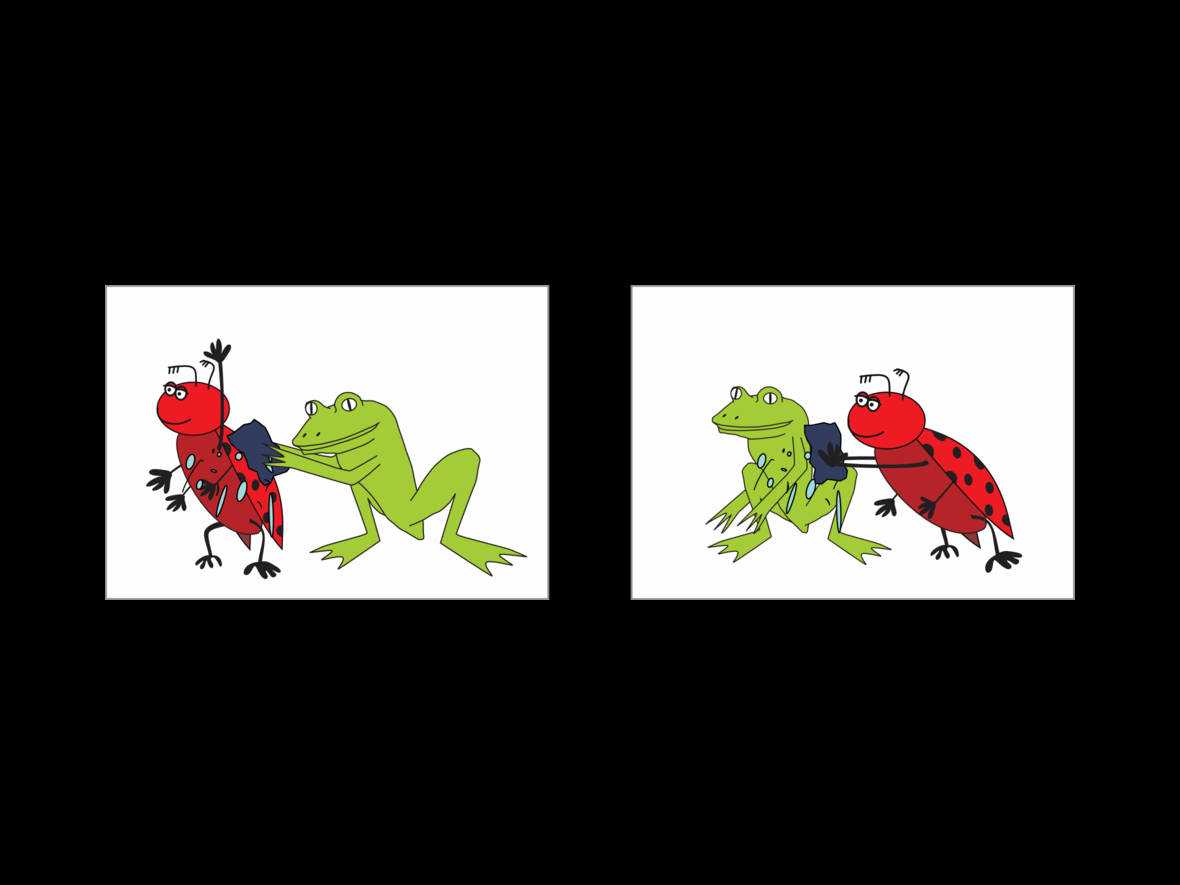
\includegraphics[width=0.75\textwidth]{pics/2_screen}
\caption{\label{2.screen} Example of a typical visual stimulus before the response}
\end{center}
\end{figure}

The spoken sentences were always posed as questions in order to elicit an immediate response.
Each question was posed in a right-branching structure (see table \ref{2.sentences} for an example).
Object-relative clauses and subject-relative clauses were presented in random order at a ratio of 2.5:1.
Questions were voiced in a natural, child-directed tone by a professional native speaker.
The question consisted of an actor, a recipient and the verb that described their interaction.
The performed action was either painting, pushing, combing, washing, pulling or catching.
The actor and recipient were selected randomly from 12 different races: Lion, rabbit, wolf, bird, fox, hedgehog, dog, tiger, ape, ladybug, bear and frog.
No two identical races appeared in the same picture.

\vspace{5mm}
\begin{table}[htb]
\begin{center}
\begin{tabular}{c|cccccccc}
Original & Wo & ist & der & K"afer, & den & der & Frosch & w"ascht?\\
Translated & Where & is & the & bug$_{OBJ}$, & who$_{ACC}$ & the & frog$_{SUBJ}$ & washes?\\
Word index & 1 & 2 & 3 & 4 & 5 & 6 & 7 & 8
\end{tabular}
\caption{\label{2.sentences} Example stimulus sentence. Top: original spelling in German. Middle: Literal translation in English. Bottom: Word index within the sentence}
\end{center}
\end{table}
\vspace{5mm}

Immediately after each response, an icon appeared below the two animal pairs.
A green checkmark, a diagonal red cross and a yellow skip symbol signified a correct response, an incorrect response and an invalid trial, respectively.
The trial feedback screen was presented for a random interval between 400ms and 800ms.

This experiment created a tradeoff between speed and accuracy.
To encourage a high level of attention and a high number of usable trials, a feedback screen was displayed at the end of each cluster.
On this screen, two bar graphs visualized response speed and accuracy during the preceding cluster.

Visual and auditory stimuli were produced by a computer running the software package Presentation (Neurobehavioral Systems, Inc., version [14.6]).
Video signal was displayed by a 17-inch TFT display at a distance of approximately 80cm.
Sound was played with a pair of semi-open headphones.


\paragraph{Analysis}

Behavioral data were analyzed with Matlab (version 2014a).
Response accuracy was evaluated for the case that subjects responded randomly.
For this purpose, accuracy was compared to the outcome of a random sequence of binary events.
I established the alpha = 0.01 confidence interval for the percentage of correct trials ($\frac{k}{n}$) that could be answered correctly purely by chance.
This calculation was implemented using the binomial fit method in Matlab: binofit(k, n, alpha).
If the upper confidence interval of this calculation exceeded the subject-specific accuracy, the subject was removed from further analysis.
Two subjects failed to exceed chance level performance, leaving 19 subjects for the analysis.

Two types of behavioral data were analyzed for group and condition effects: response time (RT) and response accuracy (RA).
Response time was measured at the condition onset, i.e. at the "'d"' sound of the sixth word.
Trials were omitted when the subject skipped or answered them incorrectly, or responded earlier than the cue.
Accuracy was calculated by dividing the amount of correct trials by the amount of total trials for each subject.

A Shapiro-Wilk test was used to test for normal-distributed residuals.
Accuracy passed this test at a p = 0.01 significance level.
The impact of the syntactic condition on response accuracy was determined with a T-test.

Any unintended bias on response time was determined by splitting RT from each subject into two groups along one of five impact factors.
The two groups were then compared with a T-test.
The five grouping factors were response side (left / right), condition (object-relative / subject-relative), the race of the actor (12) and recipient (12) and the peformed action.

\paragraph{Results}

Subjects responded after a median delay of 2.0s (quickest 5\%: 1.0s, slowest 5\%: 5.2s).
The median accuracy was 70\% (worst 5\%: 62\%, best 5\%: 94\%).
The syntactic condition had a highly significant effect on accuracy (p < 0.001, t(18) = -14.0).
No factor had a significant effect on response time (p > 0.1, F < 1.5).

\begin{figure}[h]
\begin{center}
\vspace{7mm}
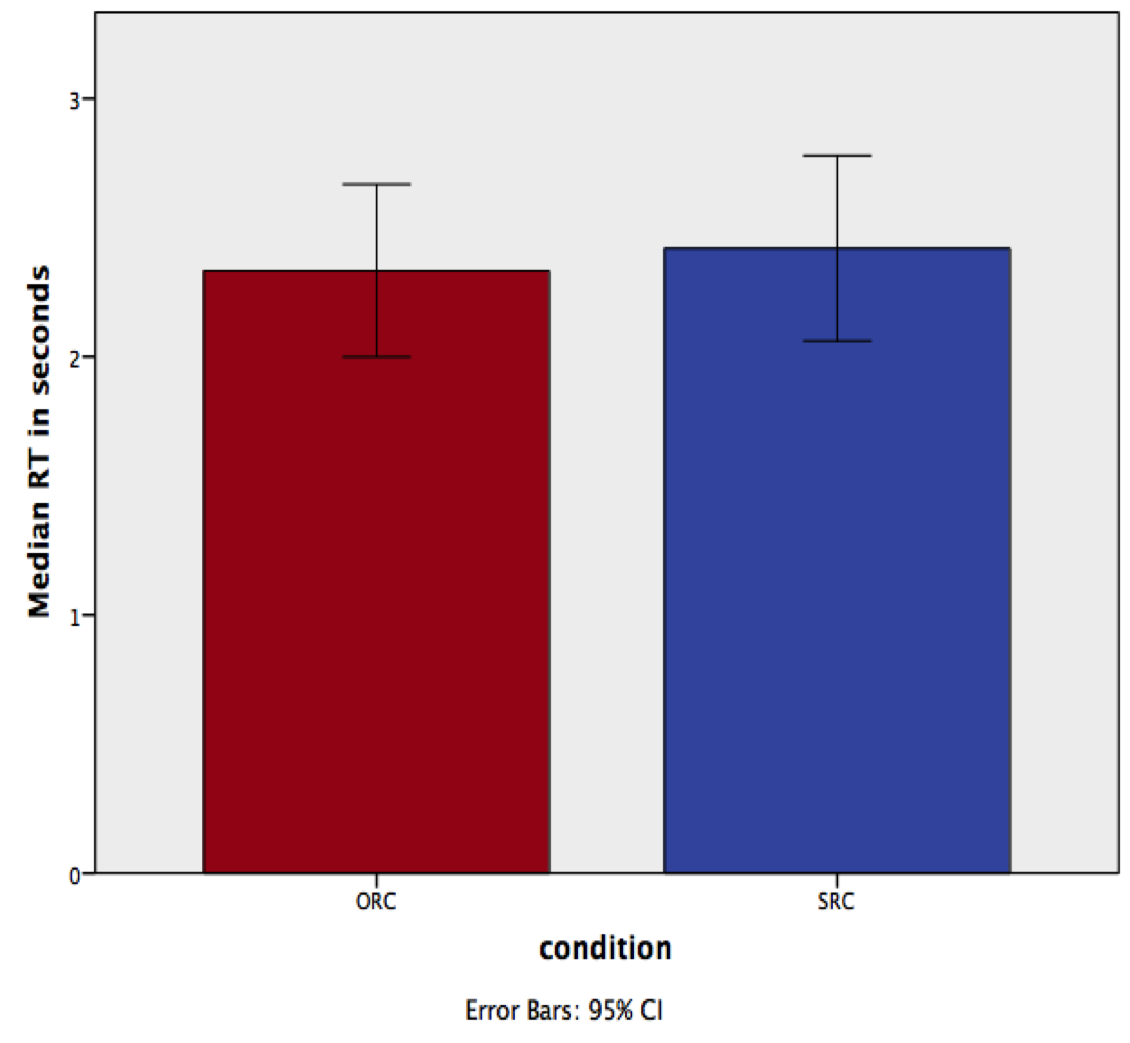
\includegraphics[width=0.45\textwidth]{pics/2_RTgraph}
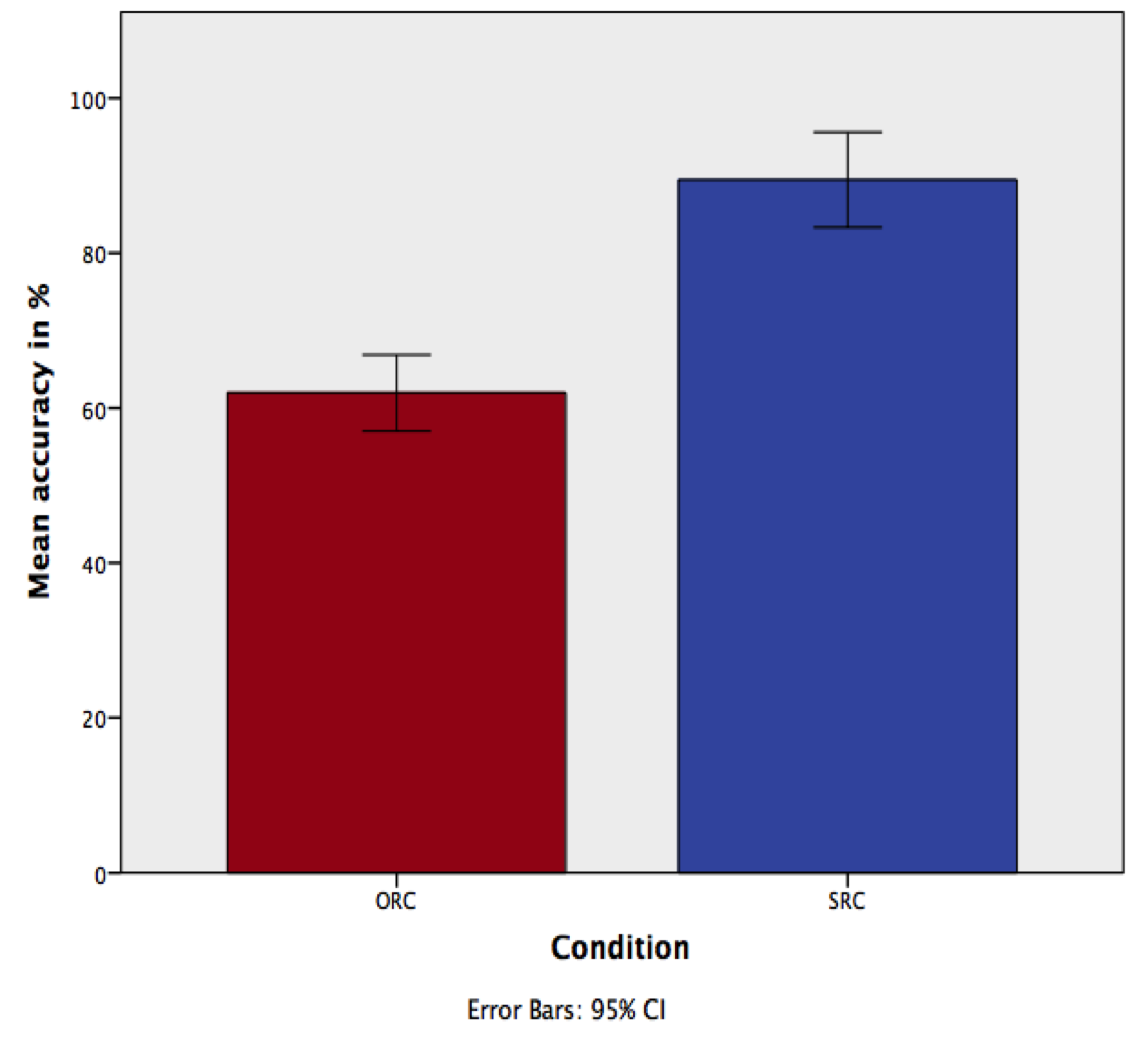
\includegraphics[width=0.45\textwidth]{pics/2_RAgraph}
\caption{\label{2.RTgraph} Chart of the grand average performances for subject-relative (blue) and object-relative (red) clauses. Left: Median response time from conditional onset. Right: Average response accuracy.}
\end{center}
\end{figure}

Post-hoc tests were conducted to reveal condition-specific accuracy values.
The average accuracy for responses to subject-relative clauses was much higher than to object-relative clauses (93\% and 64\%, respectively).
Due to the proximity to a 50\% chance level, I repeated the binomial fit test of individual accuracy, exclusively with responses to object-relative clauses.
8 of 19 subjects failed this test at a p = 0.01 significance level.
After removing these subjects from the analysis, selected tests were repeated.

Median response times remained unchanged for both conditions.
Overall accuracy in the remaining subjects improved slightly (95\% for subject-relative clauses and 68\% for object-relative clauses).
The difference in accuracy between conditions weakened slightly (p < 0.001, t(10) = -9.4).


\paragraph{Discussion}

The first goal of this pilot study was to establish an unbiased test paradigm.
The variation in grammatical elements had no undesired impact on response times.
Syntax conditions produced a strong effect in both performance metrics.
These findings support the current stimulus setup for use during MEG measurements.


The second goal of the pilot study was to determine if 10-year old children were suitable subjects for the designed task.
Accuracy levels were comparable with the findings of similar experiments.
Due to different trigger points and sentence lengths, comparisons of response times couldn't be made directly and were instead limited to comparisons of effect size.
I start by comparing our results to our spiritual predecessor, the study by [2.1].
They found no significant conditional impact on response time in the 9-10-year age bracket.
In stark contrast to our results (93\% and 64\% for subject- and object-relative clauses), their subjects were not influenced by a condition effect, with accuracy levels of 94\% in both conditions.
The good performance was met with surprise and speculation that semantic cues may have helped with sentence comprehension.
This speculation was supported by their fMRI findings, which indicated that children relied heavily on semantic-centric processing areas, rather than on pure syntax-related processing areas that adults use.
Our setup didn't include semantic cues, which puts our results more in line with other infant studies.

[2.2], for instance, measured repetition performance in 3- and 4-year-old children.
The study presented German subject-relative and object-relative clauses with two interacting people in third person, similar to our setup.
Their subjects performed with an accuracy of just 5\% (3 years) and 26\% (4 years) for object-relative clauses.
Subject-relative clauses were performed with 13\% and 31\% accuracy, respectably.
Note that these ratings represent accurate verbal repetition, and don't need to be corrected for chance level performance.

[2.3] found more accurate responses to portuguese right-branching subject- and object-relative clauses.
Subject-relative clauses were correctly answered 23\%, 50\%, 83\% and 80\% of the time (in 3-, 4-, 5- and 6-year old children, respectably).
Object-relative clauses reached only slightly lower accuracy levels of 18\%, 40\%, 75\% and 68\%, respectably.
They employed a more user-friendly approach by requiring the children to act out the posed sentences with toy animals.
Because the authors deliberately removed as many processing constraints as possible, these accuracy levels can be considered upper performance limits on these age brackets.

6 to 8 year old children solved syntactic problems with higher complexity in the study by [2.4].
The experimental design varied two syntactical factors and one contextual factor.
One syntactical factor, "'question"', varied English object- and subject-relative clauses, coinciding with our setup.
Object-first and subject-first clauses were responded with an accuracy of 64\% and 83\%, respectably.

Response time and accuracy performance indicates that the 10-year age bracket was successful in selecting subjects with an incomplete dorsal tract II.
Compared to typical adults, our subjects performed considerably worse in both accuracy and response time.
Compared to younger children, our subjects performed condsiderably better in subject-relative clauses.

42\% of our subjects failed to perform better than chance level when the task required a fully-developed AF.
I have no sufficient reason to assume that these subjects were using a random-button strategy.
If anything, the weakened condition effect indicates that these performances were due to honest mistakes.
Hence, there is no reason to exclude subjects with chance-level performances to object-relative clauses.


Finally, the pilot study revealed a few design flaws as well.

First, sentences differed systematically between conditions even before the intended condition cue.
The syntactical condition reverses the order of pronouns, creating an opposition between "'der den"' and "'den der"'.
To prevent confounding effects from different content, the initial sentence fragment needs to be identical at least across conditions, and, preferably, across trials as well.
Ideally, the distance between the end of this identical sentence fragment and the conditional cue point should be as short and invariant as possible.

Second, our sentence structure contained a theoretical loophole.
With sufficient time and wit, subjects could develop an alternative strategy that doesn't require syntactic processing of the whole sentence.
The alternative strategy exploits the fact that the minimum information for a correct decision is already available at the fifth word (see table \ref{2.1.sentences}).
Subjects only needed to complete three sequential steps:
First, attending only to the left of the two pictures.
Second, waiting until the fourth word is spoken.
If the mentioned animal was displayed as actor, the left button would be correct and vice versa.
Third, using the fifth word to execute the previous or the reverse button mapping.
If the mentioned word was a "'der"', the previously correct button remained correct and could be pressed immediately.
If the mentioned word was a "'den"', the previously wrong button had to be pressed for a correct result.
This strategy could potentially reduce the task into a simple series of motor preparation and pattern matching.
Complex syntactic processing and, presumably, the use of pSTS and dorsal pathway II would be circumvented.
Employing this strategy could create suspicious behavioral results in the form of systematically reduced and less varied response times.
This flaw was the main reason for the redesign of stimuli for the main study.
\chapter{Methods}\label{methods}

\section {Participants and stimuli}

\subsection{Participants}

18 children and 22 adults were recruited from the internal participants database.
Subjects were selected if they spoke German as native language, if their language development was unremarkable, if their handedness score was above 70, if they fulfilled the prerequisites for MRI scans, and if their medical history was free of cognitive abnormalities.
4 children and 4 adults dropped out inbetween sessions of the study.
Two children were excluded from the analysis because their behavioral performance was at chance level.
12 children (5 female) and 18 adults (9 female) were left for the subsequent analysis.
Children were aged between 9y11m and 10y9m and described as right-handed by their parents.
Adults were aged between 22 and 33 years and scored between 73 to 100 (median: 95) on the laterality quotient test \cite{3.1.LQ}.
The point of reference for these ages is the time of the MEG session.
Parents gave written informed consent and were compensated with 40\euro \ for the MEG session and 7,50\euro \ for the MRI session.
Children agreed to participate in the study and were compensated with a 10\euro \ gift voucher for each session.
Adult participants were compensated with 20\euro.
All experimental procedures were approved by the University of Leipzig Ethical Review Board.


\subsection{Task}

The study consisted of two sessions: an anatomical MRI acquisition (duration: 50 minutes) and an interactive magnetoencephalographic measurement (typical duration: 90 minutes).
Since they took place in two different locations, there was a delay (median: 98 days, maximum: 243 days) between the two sessions.

The MRI session is described in detail in section 3.2.2.

The MEG session consisted of two sections: a tutorial section and a main section.

\paragraph{MEG tutorial section}

First, the tutorial section described the usage of the interface.

Second, subjects needed to respond to an example stimulus with the spoken sentence written out below the screen.

Third, three example trials followed without the written sentence.

Fourth, an artificially incomprehensible sentence was presented together with otherwise innocuous visual stimuli.

When subjects pressed either response button instead of skipping the trial, they were instructed with the skip function.

Finally, a series of randomized tutorial trials followed.
When subjects showed behavioral proficiency of the task, the tutorial ended prematurely.
Two thresholds for proficiency were possible: either an average response time below 3000ms and an accuracy score above 80\%, or an accuracy score above 88\%.
Either threshold could only be reached after completing at least 5 or 8 trials, respectively.
When none of these thresholds were met, the tutorial ended after 36 trials.

\paragraph{MEG main section}
The main section was used for MEG acquisition and consisted of 304 trials grouped in two blocks.
There was a scheduled break between the blocks (usually 1-2 minutes) which included interaction with the research assistant.
Subject-specific trial randomization was performed before the task.
All stimuli-related randomization tasks were implemented with a time-seeded Mersenne-Twister approach in Python 2.7.
Randomization contained two exceptions: neither the same image nor the same sentence could be played twice in a row.
Each block consisted of 8 clusters.
Subjects were shown a feedback screen at the end of each cluster, summarizing their performance throughout the recent cluster.
Since manual intervention was necessary to proceed to the next cluster, subjects frequently used this opportunity for a tiny break (typically 5-20 seconds).
Each cluster consisted of 19 trials.

\paragraph{Structure of a single trial}
Each trial started by showing two pictures side-by-side.
In one picture, one of the animals performs a social action on the other animal.
In the other picture, the roles are reversed.
10ms later, the spoken question started playing.
The subject could respond by pressing one of the direction buttons or the skip button.
There were two direction buttons, left or right, signifying that the left or right image contained the answer to the question.
The skip button was used to mark the trial as invalid for further analysis, and excluded the trial from performance feedback.
This response was the correct choice when the subject was distracted or failed to comprehend the question immediately.
This opened a minor pitfall: subjects could have gotten perfect scores by just pressing the skip button each time.
Fortunately, none of the subjects discovered this opportunity.
The trial ended with an auditory and visual feedback.


\subsection{Visual stimuli}

\paragraph{Character motivation}
A set of visual stimuli consisted of a two side-by-side images on black background.
Each image depicted two different animals on a white background.
I selected selected social activities that were only plausible for antropomorphised characters, not for their real animal counterparts.
Antropomorphization includes the use of their front limbs for object manipulation and standing on their hindlegs.
These measures are introduced to prevent associations with real-world animalistic behavior.
For example, a lion "'catching"' a monkey could resemble predatory behavior.
This association with chasing and killing would introduce a semantic bias against the reverse interaction: a real-life monkey "'catching"' a lion is much more implausible than the reverse.
To further detract from a naturalistic view, the animals were represented in a cartoon style.
To prevent unnecessary stress on this interpretation, I only selected animals whose real-life counterparts were approximately equally sized.

\begin{figure}[h]
\begin{center}
\vspace{7mm}
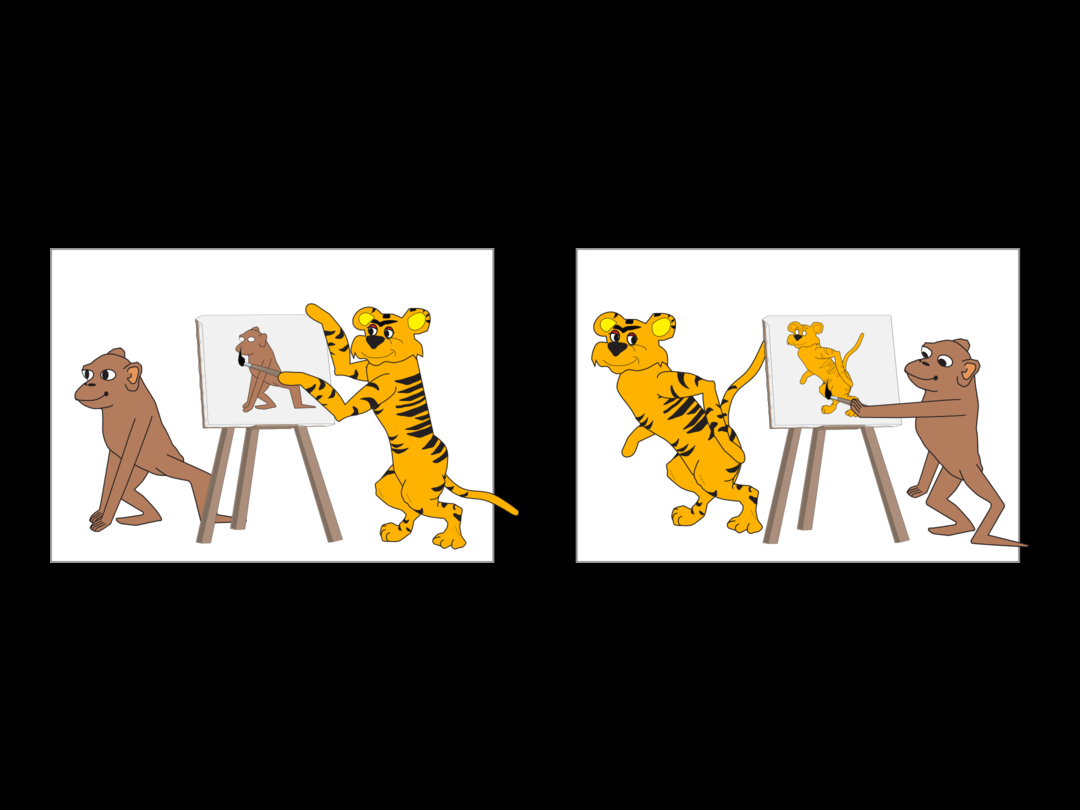
\includegraphics[width=0.5\textwidth]{pics/3_1_screen}
\caption{\label{3.1.screen} A typical visual stimulus, featuring two pairs of animals.}
\end{center}
\end{figure}

Image components were adapted with permission and kind advice from \cite{3.1.animals}.
Modifications were performed with Inkscape.

\begin{figure}[h]
\begin{center}
\vspace{7mm}
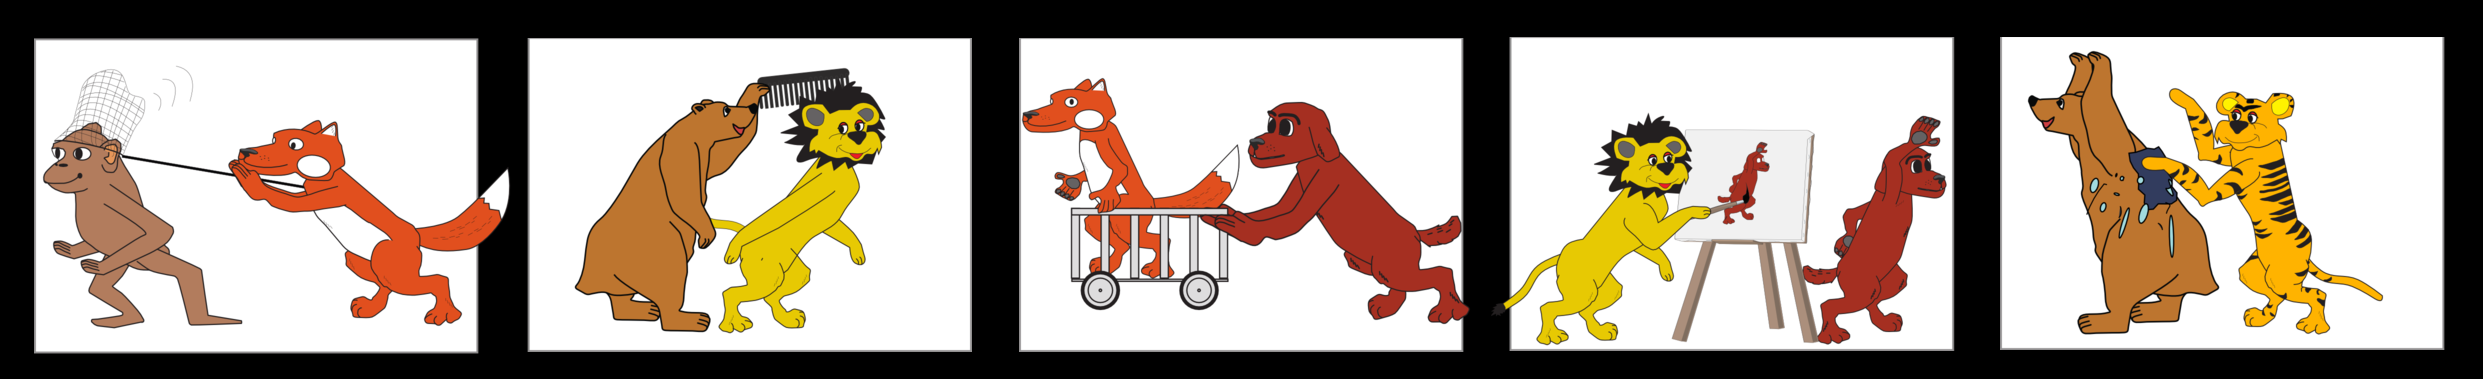
\includegraphics[width=0.99\textwidth]{pics/3_1_activities}
\caption{\label{3.1.activities} Illustrations of all five animals performing their social activities. From left to right: catching, combing, pushing, painting and washing}
\end{center}
\end{figure}

\paragraph{Trial feedback}
Immediately after each response, an icon appeared below one of the two displayed animal pairs.
The presented side was determined by the subject's response.
In the case of the skip button, the icon appeared at the same height as the others, but in the middle of the screen.
A green checkmark, a diagonal red cross and a yellow skip symbol signified a correct response, an incorrect response and an invalid trial, respectively.
The trial feedback screen was presented for a random interval between 400ms and 800ms.


\begin{figure}[h]
\begin{center}
\vspace{7mm}
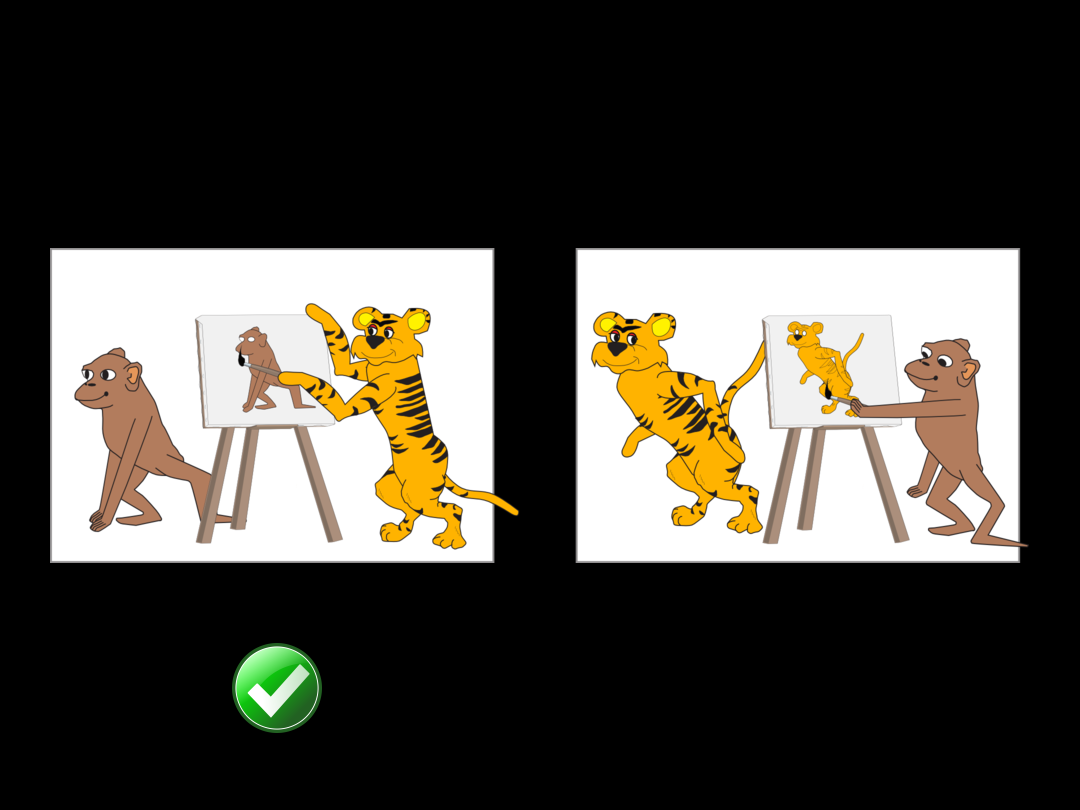
\includegraphics[width=0.5\textwidth]{pics/3_1_feedback}
\caption{\label{3.1.feedback} The visual feedback to a correct response.}
\end{center}
\end{figure}

\paragraph{Cluster feedback}
In this experiment, there was an obvious tradeoff between speed and accuracy.
To encourage a high level of attention and a high number of usable trials, two bar graphs visualized performance speed and accuracy (see Fig. \ref{3.1.clusterfeedback}).
In order to maximize the amount of usable trials for further analysis, the visualization valued accuracy much more than response time (see Fig. \ref{3.1.feedbackGraphs}).

\begin{figure}[h]
\begin{center}
\vspace{7mm}
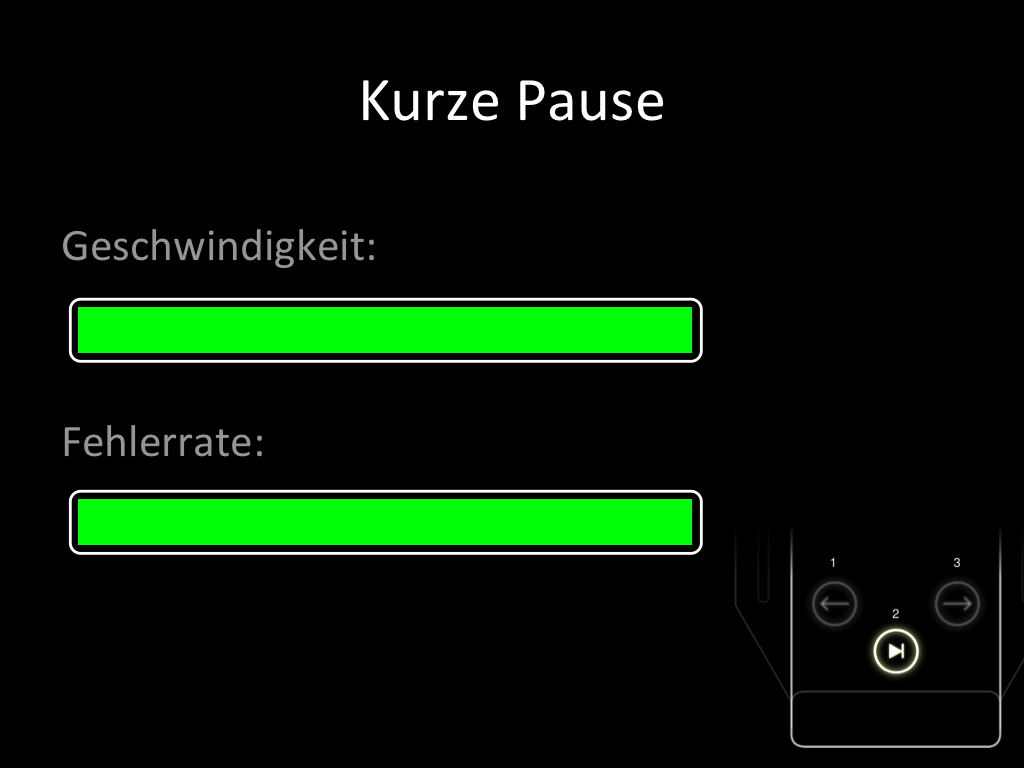
\includegraphics[width=0.5\textwidth]{pics/3_1_clusterfeedback}
\caption{\label{3.1.clusterfeedback} An ideal cluster feedback screen that appears after completing 19 trials. Upper bar: speed, lower bar: accuracy. Bottom right: indicator to  press the skip button to advance}
\end{center}
\end{figure}

\begin{figure}[h]
\begin{center}
\vspace{7mm}
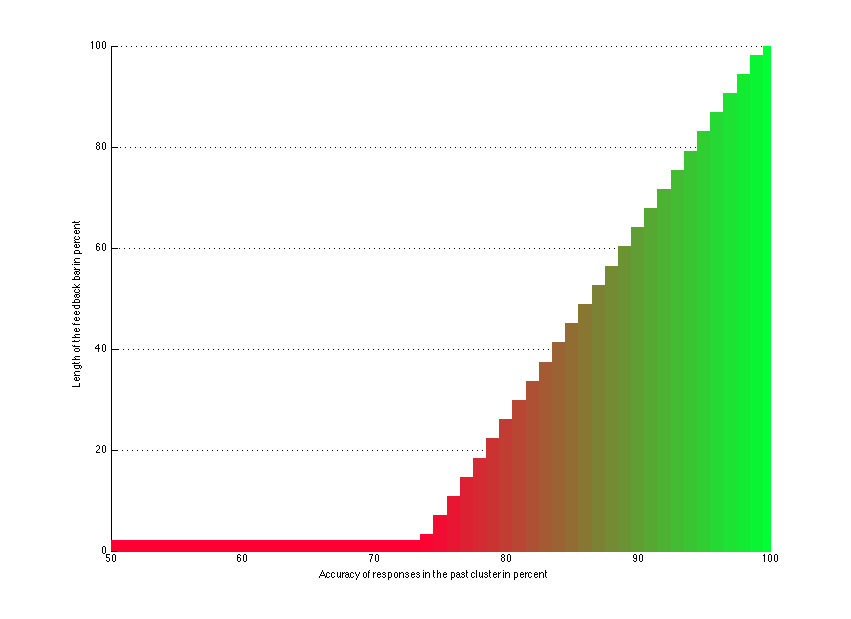
\includegraphics[width=0.45\textwidth]{pics/3_1_feedbackGraphAccuracy}
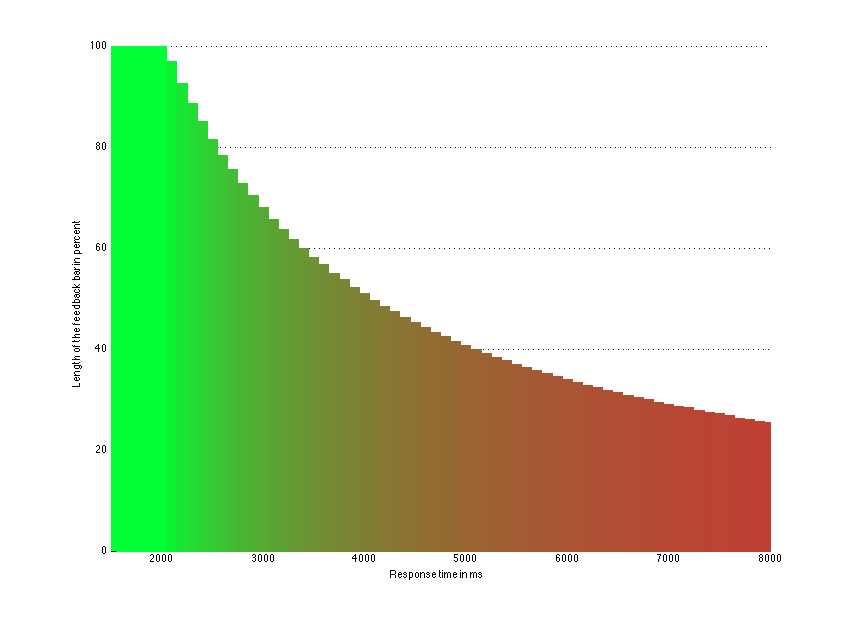
\includegraphics[width=0.45\textwidth]{pics/3_1_feedbackGraphRT}
\caption{\label{3.1.feedbackGraphs} Relation between performance and displayed feedback bars. Performance (left: RA, right: RT) is drawn along the X-axis, and length of the bars in \% is drawn along the Y-Axis.}
\end{center}
\end{figure}

\subsection{Auditory stimuli}

\paragraph{Sentence content}
Each pair of images was presented with a spoken question.
The question format fit well with the stimulus-response paradigm, and allowed the sentences to be identical until the conditional article ("'den"' or "'der"') appeared.
Syntactically, the sentences used an equal number of subject-relative and object-relative clauses.
In order to minimize confounding effects, these two conditions were designed to show as little auditory distinction as possible.
The structure of the final sentences is displayed in table \ref{3.1.sentences}.

\begin{table}[htb]
\vspace{5mm}
\begin{center}
\begin{tabular}{c|cccccccc}
Original & Wo & ist & das & Tier, & das & der & Tiger & malt?\\
Translated & Where & is & the & animal$_{OBJ}$, & which & the$_{NOM}$ & tiger$_{SUBJ}$ & paints?\\
Word index & 1 & 2 & 3 & 4 & 5 & 6 & 7 & 8
\end{tabular}
\caption{\label{3.1.sentences} Example stimulus sentence. Top: original spelling in German. Middle: Literal translation in English. Bottom: Word index within the sentence.}
\end{center}
\end{table}

\paragraph{Tutorial sentences}
During the pilot study, children often assumed that the every sentence was a subject-relative construction, miscategorizing "'den"' for "'der"'.
Tutorial sentences made the two animal nouns explicit, so that all sentences were structured in the format "'Where is the monkey that is caught by the dog?"'.
While this setup was creating strong auditory differences, it was easier to comprehend.
If the children didn't notice the difference by the eighth tutorial trial, the research assistant repeated the question with an exaggerated "'den"' pronounciation.

\paragraph{Audio format}
Sentences were spoken by a professional female native speaker in an uni\-so\-nous and moderately child-directed prosody.
Recording and playback was performed at a sampling rate of 44100Hz with one channel.
Loudness of each sentence was normalized.
Overall loudness was adjusted to 50db above each subject's individual hearing threshold.

\paragraph{Trial feedback}
Immediately after each response, one of two short sounds played.
The sounds were extracted from Microsoft Windows XP.
The "'external device plugged in"' icon (two bell sounds in ascending tone) and the "'external device removed"' icon (two bell sounds in descending tone) represented correct and incorrect responses, respectively.
No sound was played after the skip button.

\subsection{Experimental setup}
The participants were seated on a comfortable chair, inside a shielded, dimly-lit cabin.
Visual and auditory stimuli were produced by a computer running Presentation (version 14.0) at 60Hz refresh rate and 1024x768 resolution.
Video signal was routed through a video splitter MSV1235 into a Panasonic PT-D7700 projector.
Audio signals were generated by a Soundblaster Audigy 2 ZS [SB0350].
An audio amplifier (Compumedics, Hamburg, Germany) drove a pair of TIP-300 loudspeakers (Nicolet, Biomedical Madison, WI, U.S.A.).
Sound was routed through a pair of plastic tubes (50cm length, approx. delay of 1.6ms)
Sound arrived in the subjects' ears via ER3-14A/B earplugs (Etymotic Research Inc., Elk Grove Village IL, U.S.A.).

\section{Data acquisition}

\subsection {MEG}
MEG data were collected with an Elekta Neuromag VectorView\textsuperscript{\textregistered} MEG scanner in Bennewitz, at the development unit for Magnetoencephalography and Cortical Networks, Institute for Cognitive and Brain sciences, Leipzig, Germany.
The scanner comprised 306 MEG-channel sensors (102 magnetometers, 204 planar gradiometers).
Sensors were tuned prior to each MEG recording session to limit noise levels to approximately 2.5 fT/cm Hz^-0.5.
Sensors that became very noisy during a recording block would be individually re-tuned at the next inter-block break, either by using the fine-tuning options or the selective heating function.
Continuous MEG data were recorded at 1000 Hz sampling rate (330 Hz lowpass filter).

Prior to data acquisition, all metal and other potential sources of electromagnetic interference were removed from participants.
Quality of recording was confirmed by visual inspection of a live view of MEG recording before each session without the subject present.
Electro-oculogram (EOG) and electrocardiogram (ECG) time-series were recorded simultaneously with MEG to track potential noise sources and artifacts.
Five head position indicator (HPI) coils were attached to the participant's forehead and a Polhemus stylus and digitizer device were used to record the locations of fiducial points (right and left pre-auricular points (RPA, LPA) and nasion), the HPI coils, and between 150 and 200 extra digitizer points on the head surface.
Prior to the recording of each stimulus block, head location in the scanner was measured with an automatic process that detected the coils.
Continuous HPI recorded any head movements during data acquisition.

\subsection {MRI}
Anatomical magnetic resonance imaging (aMRI) data were collected with a 3.0 Tesla TIM Trio scanner, located at the Max-Planck-Institute for Cognitive and Brain sciences.
Two scans were acquired from each participant in one session: A T1-weighted scan and a T2-weighted scan.
The T1-weighted scan used the magnetization-prepared rapid gradient echo (MPRAGE, \cite{3.2.mprage}]) sequence (flip angle = $9\textdegree$, TR/TE/TI = $2300ms/2.96ms/900ms$).
This scan was oriented transverse (176 slices) with an isotropic resolution of 1mm.
The T2-weighted scan used the SPACE sequence by \cite{3.2.space} (flip angle = $120\textdegree$, TR/TE = $3200ms/402ms$).
This scan was oriented transverse (176 slices at 1mm) with an inplane resolution of 0.5mm x 0.5mm.
All scans used a 32-channel head coil for the acquisition.


\section{Data analysis}

Data were preprocessed with the three software packages: Elekta Neuromag\textsuperscript{\textregistered} MaxFilter (version 2.2, \cite{3.3.MNE}), Matlab (version 2014a) and MNE-Python (version 0.8.6, \cite{3.3.MNEpython}).

\subsection{Behavioral data}

Two types of behavioral data were analyzed for group and condition effects: response time (RT) and response accuracy (RA).
Response time was measured at the condition onset, i.e. at the "'d"' sound of "'den"' or "'der"' (in the subject-relative clause or the object-relative clause, respectively).
Trials were omitted when the subject skipped or answered them incorrectly.
Trials were also omitted if the response took longer than 4000ms.
This procedure removed 11.1\% of the childrens' trials, and 2.5\% of the adults' trials.

RT and RA were determined for each subject separately from the remaining trials.
Both metrics were tested for the requirements for an analysis of variance (ANOVA).
Normality of the residuals was tested with a Shapiro-Wilk test \cite{3.3.swtest}, implemented in Matlab.
Equality of variances was tested with a Levene test\cite{3.3.levtest}, implemented in SPSS.
RA data failed the normality test.
To include RA data in the following analysis, they were transformed to fit a normal distribution.
This transformation was accomplished with the inverted sigmoid function:
\[ \hat{a} = - log( \frac{1}{a} - 1 ) \]
All results from the ANOVA were transformed back into milisecond space with the sigmoid function:
\[ r = \frac{1}{1+e^{-\hat{r}}} \]


\subsection{Sensor-space activity}

\paragraph{Preprocessing and HPI correction}
Signal-space separation \cite{3.3.SSS} was used to reduce noise in the data by suppressing magnetic interference coming from outside and inside the sensory array.
MEG recordings were corrected for HPI movements, and co-registered across blocks to the inital head position for each individual.
All of these steps were computed with MaxFilter.
Data were then subjected to a 0.4Hz FIR highpass filter (Hamming window design, 4367 coefficients, -130db suppression at 0Hz, -3db at 0.4Hz,processing in Matlab) to remove slow trends.

\paragraph{Artifact removal}
MEG channels with abnormally high noise levels as identified by visual inspection were rejected from further analysis. A median of 1 channel (maximum: 3 channels) was removed.
The resulting pre-processed data contained major artifacts from spontaneous channel jumps, electrocardiographic (ECG) activity and electrooculographic (EOG) activity.
Jump amplitudes were detected by selecting peaks in the z-transformed continuous data that exceeded a threshold of 12 standard deviations.
Segments of 2 seconds in the pre-processed continuous data were rejected if any magnitude channel exceeded an amplitude of $6\cdot10^{-12}T$ (gradiometer channels: $4\cdot10^{-12}\frac{T}{cm}$).
Continuous data were then decomposed into independent components (ICA) that explained 99\% of the variance.
Components that correlated with EOG or ECG channels were removed with the MNE methods $preprocessing.ica\_find\_ecg\_events()$ and $preprocessing.ica\_find\_eog\_events()$, respectively.
ICA-based correction removed an average of 2.1 components per subject and block (minimum: 1, maximum: 4).
The remaining ICA components were used to reconstruct continuous data.

\paragraph{Epoching}
The main trigger was set at the condition onset (described in section 3.1.4).
Epochs were created between 1000ms before and 4000ms after the main trigger.
An epoch was rejected if the trial was skipped, or answered too slow (more than 4000ms) or answered incorrectly.
This procedure yielded an average of [] trials in children and [] trials in adults.
Data were filtered before epoching with a 45Hz FIR lowpass for visualization purposes only.

\paragraph{Establishing time windows of interest}
The condition effect was used to determine suitable time windows.
Selecting data purely based on contrast will include spurious differences as well as the condition-based differences in activity.
Since there the subsequent statistical analysis compares the same contrast, it is prone to overestimate the condition effect.
This problem was resolved with a cluster-level permutation comparison.
Spurious differences in activity should vary randomly between trials and subjects, while the condition contrast is expected with a roughly equal delay and duration.
Since the group had a strong impact on RT (see [4.1.1]), effective time windows were estimated separately for children and adults.

First, the mean was computed for data from all trials, separately for each subject and condition.

Second, sensor data was pooled by calculating the mean within each of three sensor groups (from parietal, temporal and frontal locations).
These locations were selected according to previous literature findings.
Finally, clusters were computed by the MNE function $stats.permutation\_cluster\_test()$ \cite{3.3.clustertest}.
The function was run with 500 permutations, and an t-threshold of 2.0.

For visualization purposes, grand average activity was also calculated for each sensor group and condition, separately for children and adults.

\begin{figure}[h]
\begin{center}
\vspace{7mm}
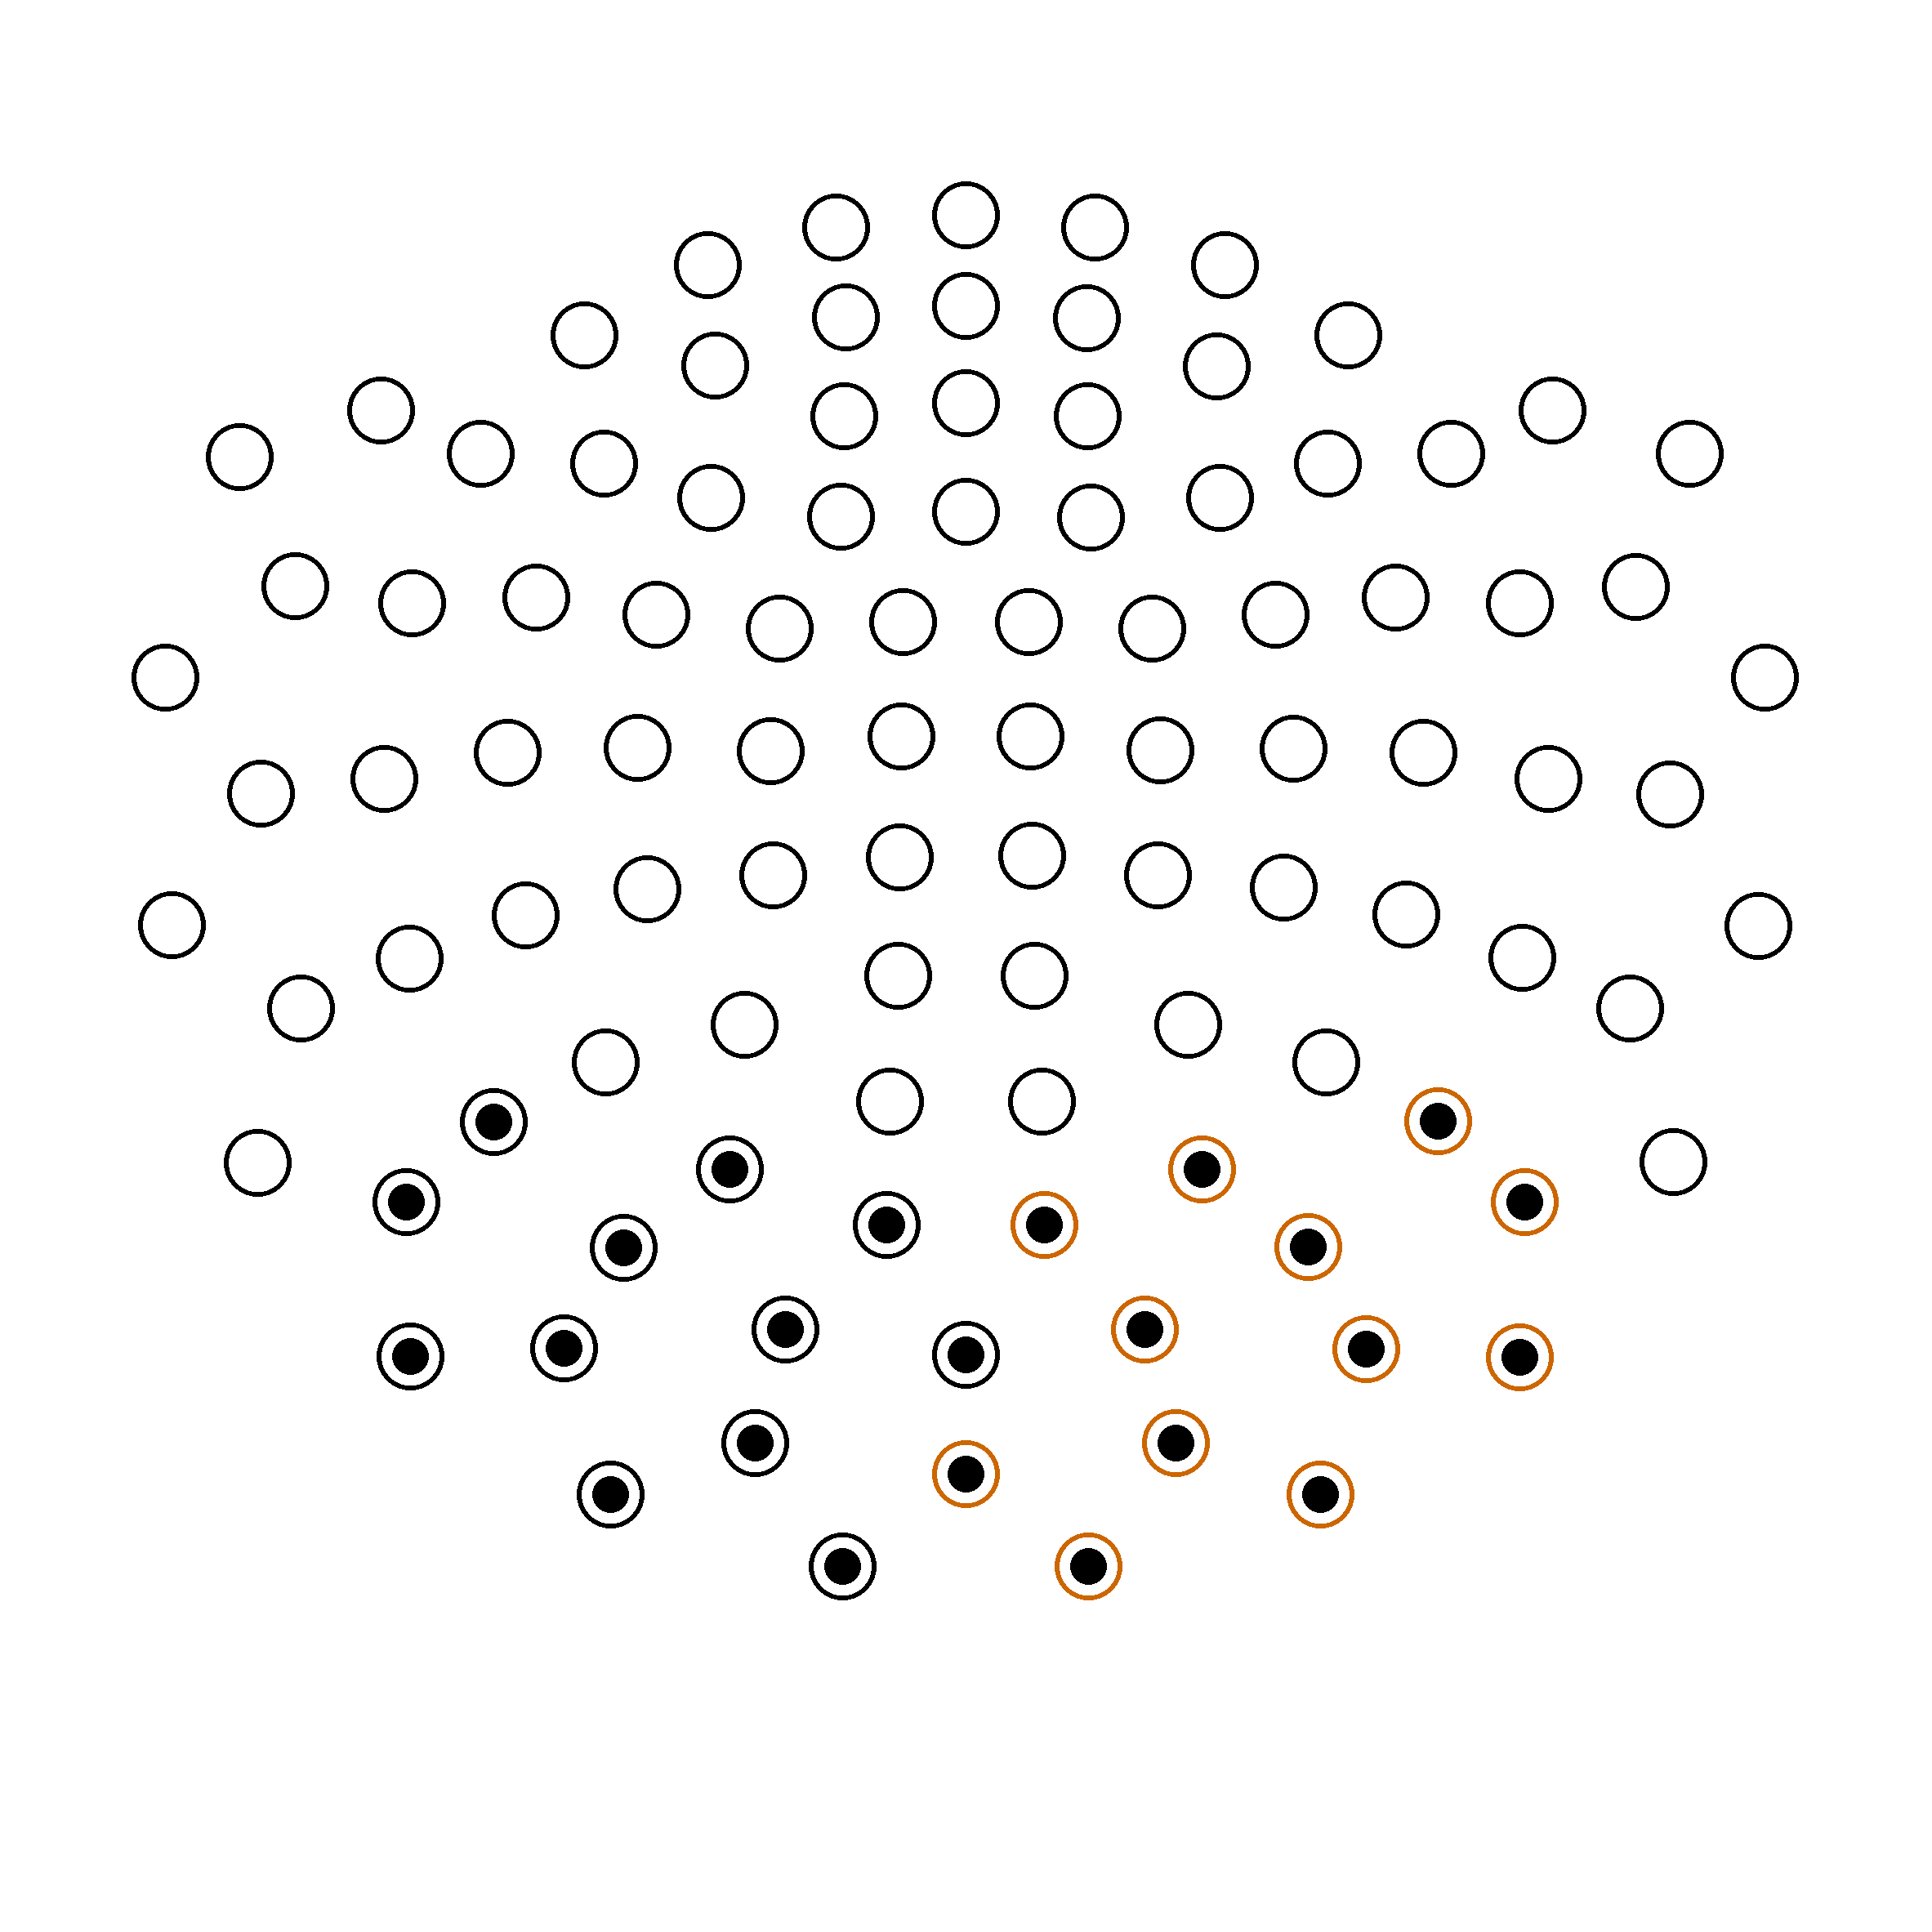
\includegraphics[width=0.24\textwidth]{pics/3_3_occipital_sensors}
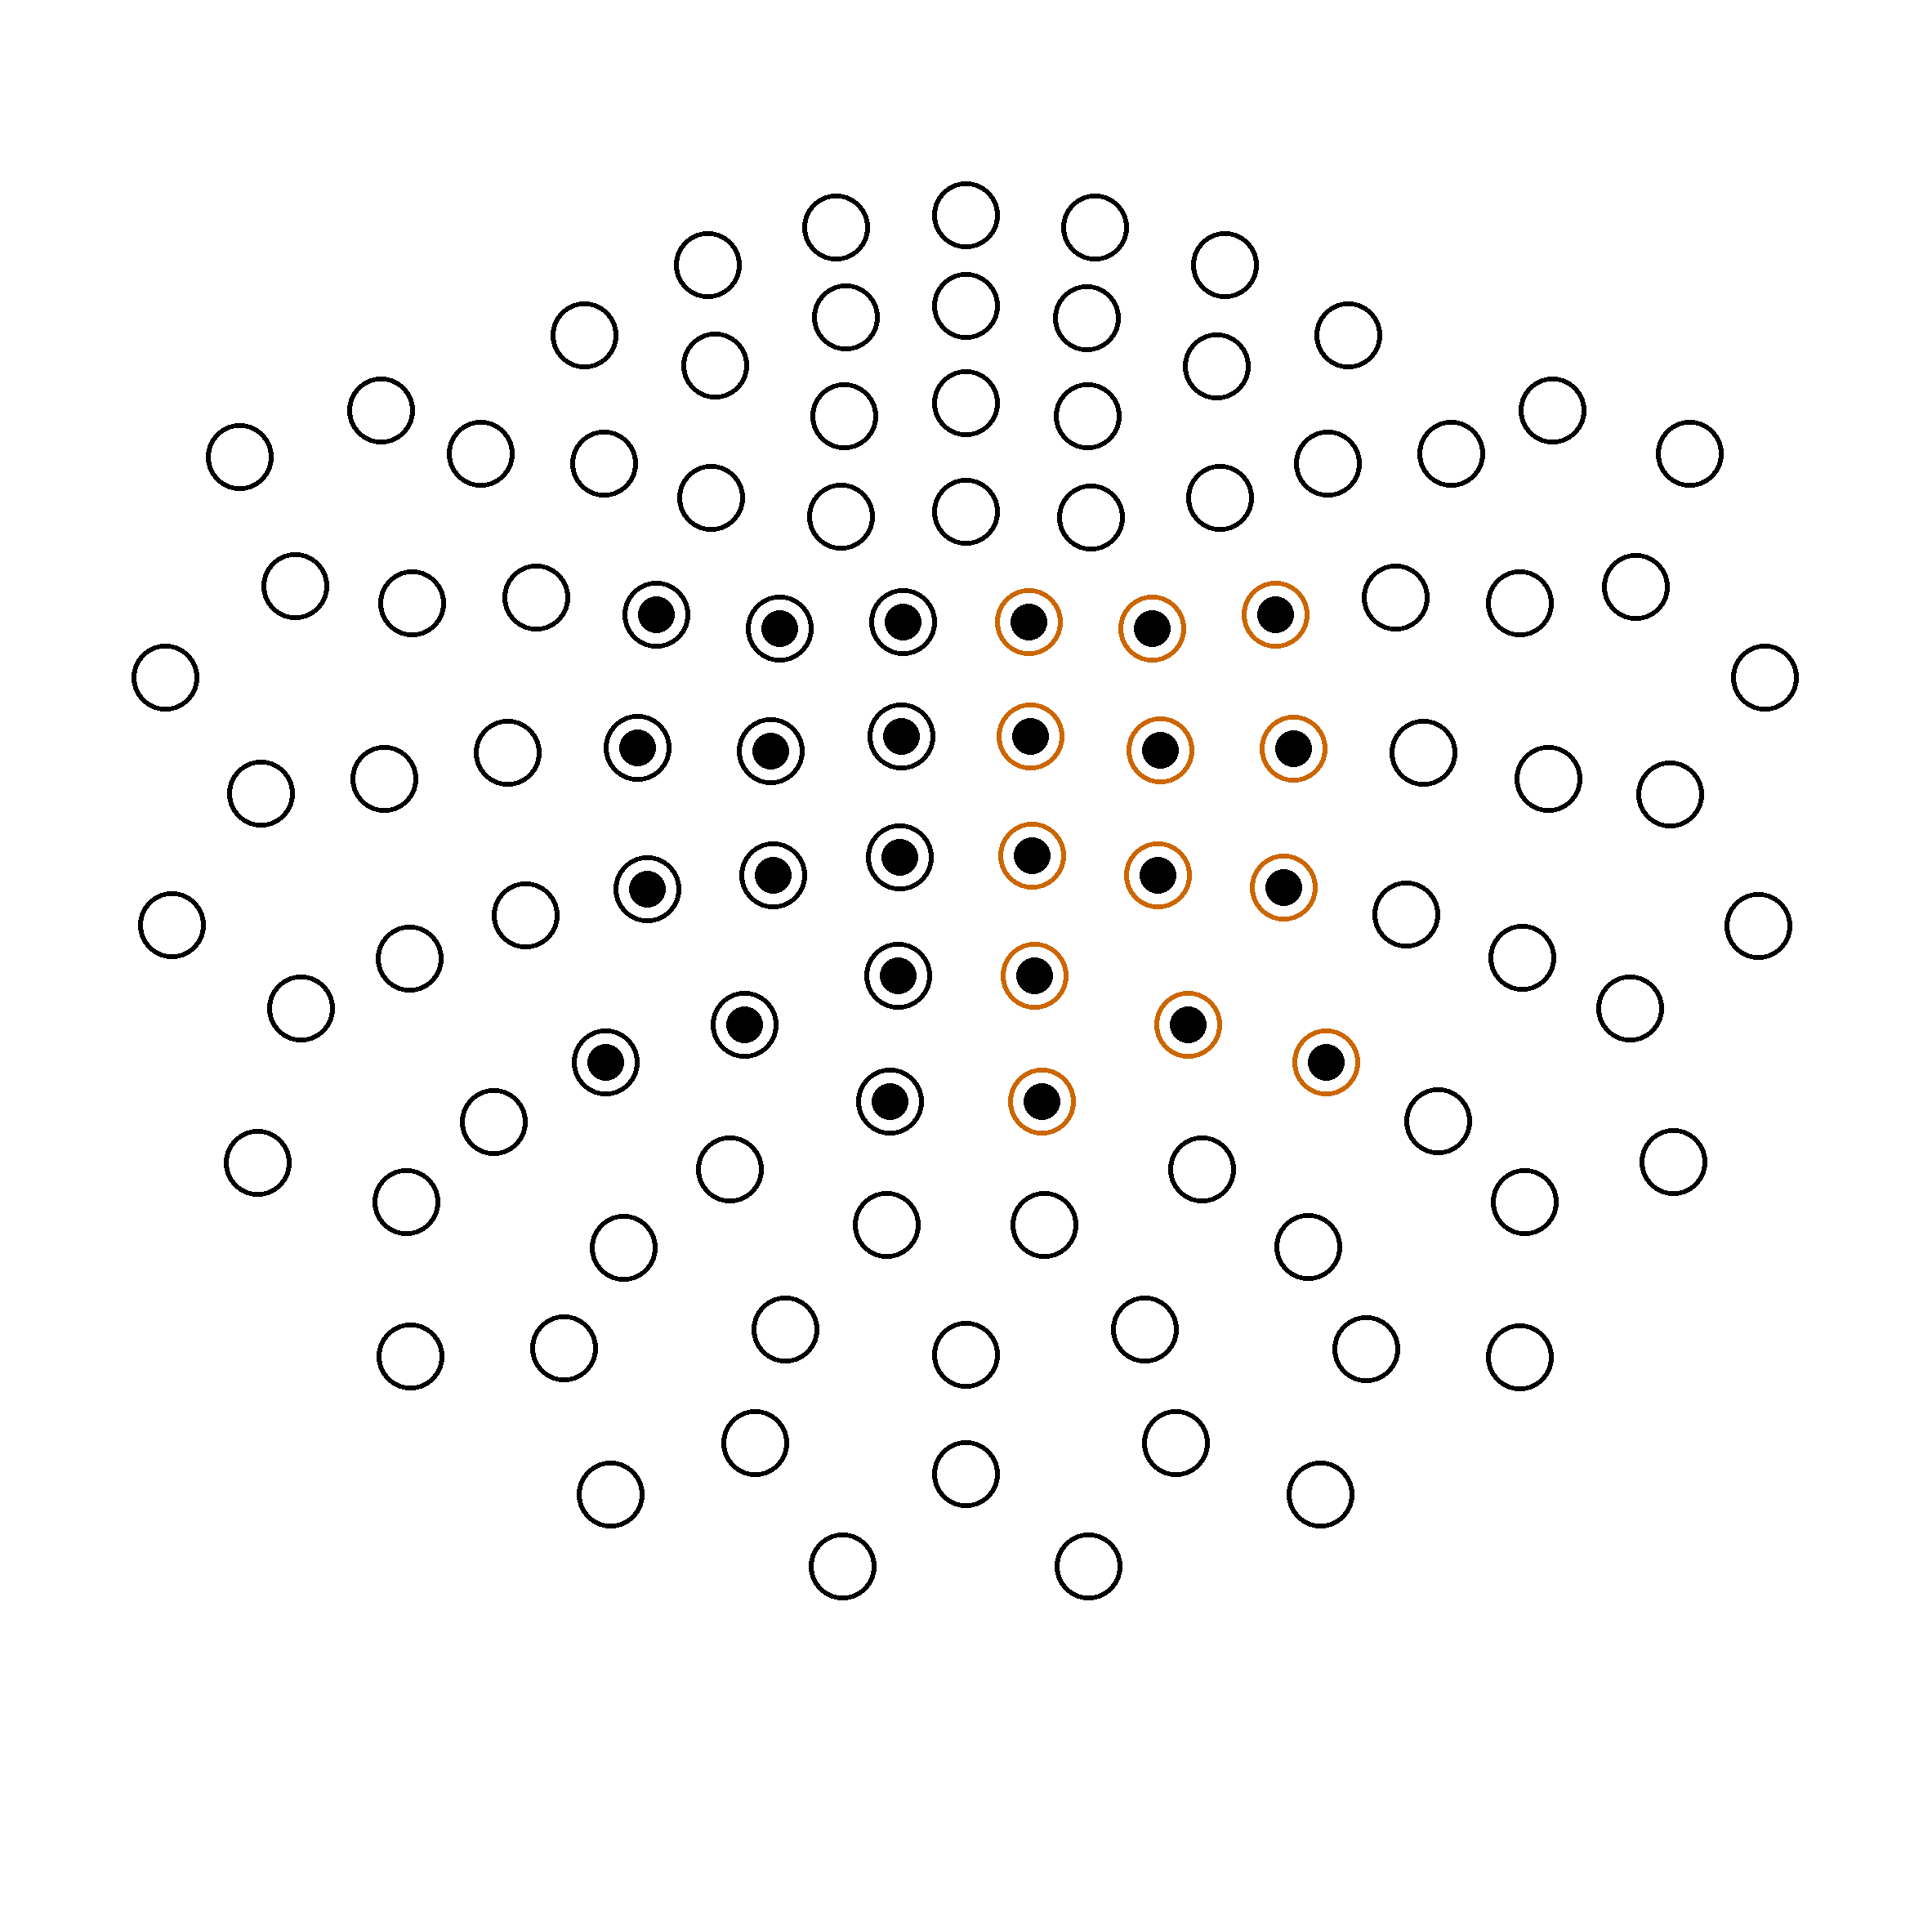
\includegraphics[width=0.24\textwidth]{pics/3_3_parietal_sensors}
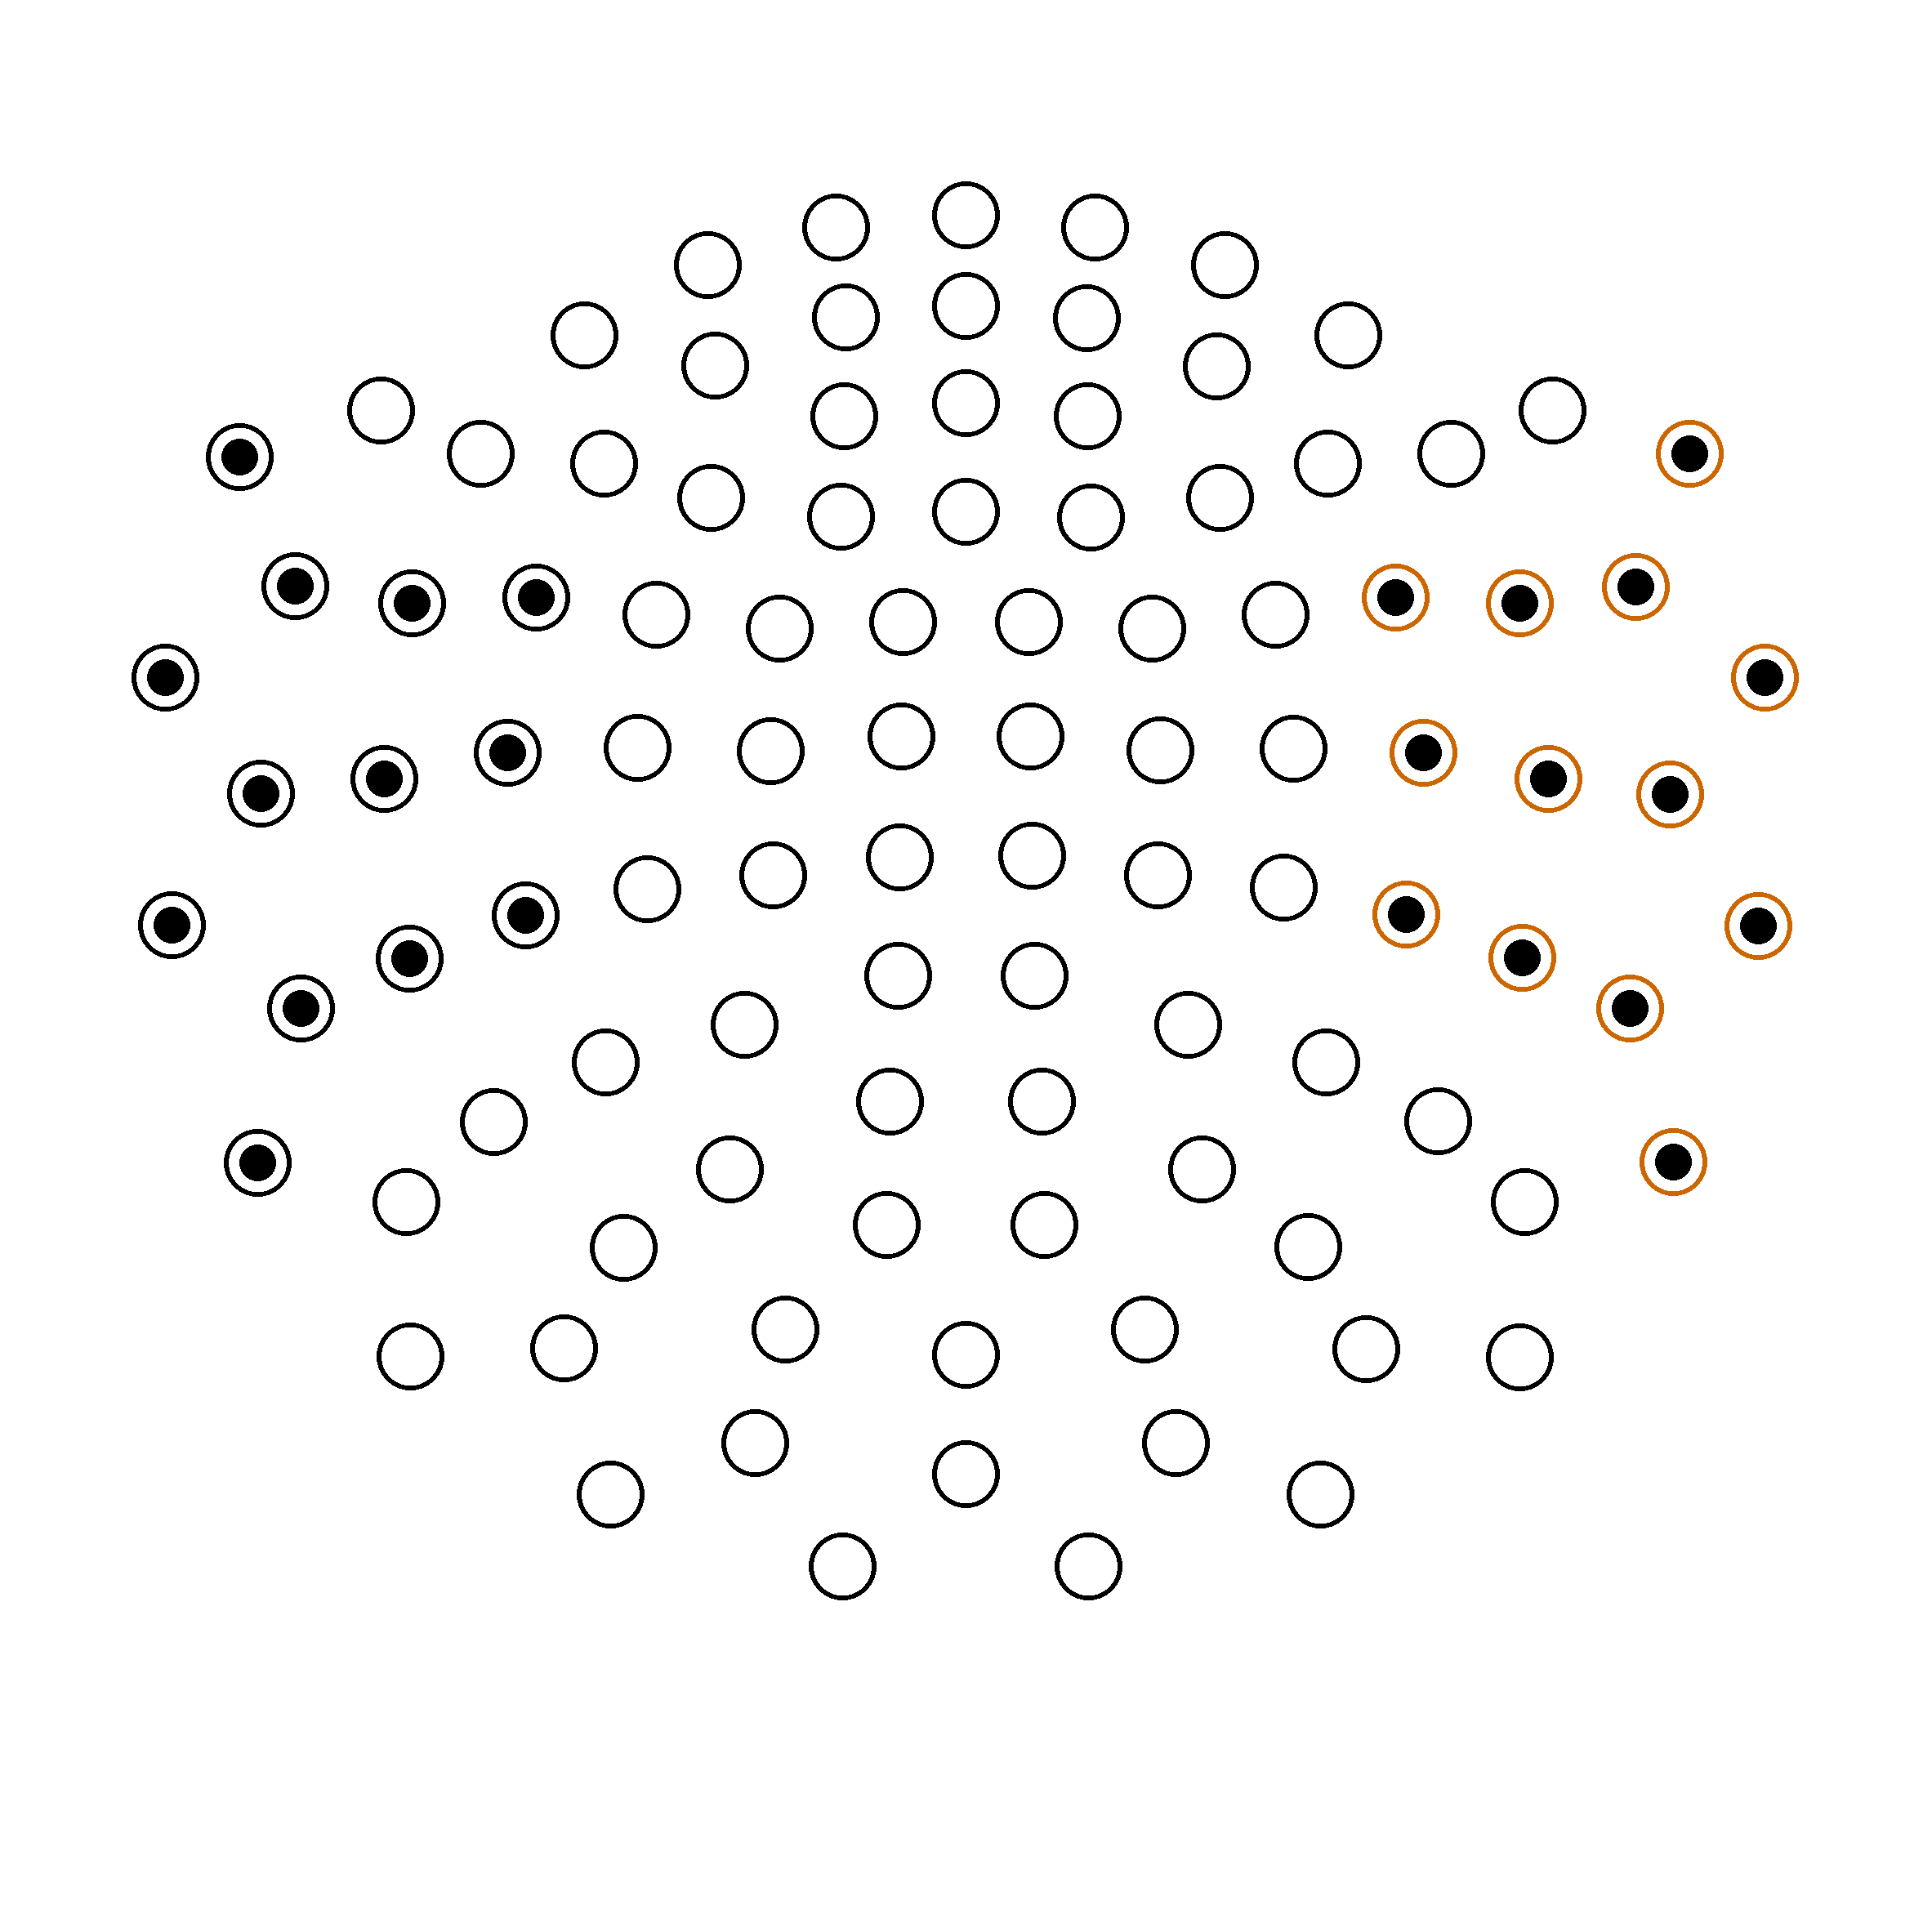
\includegraphics[width=0.24\textwidth]{pics/3_3_temporal_sensors}
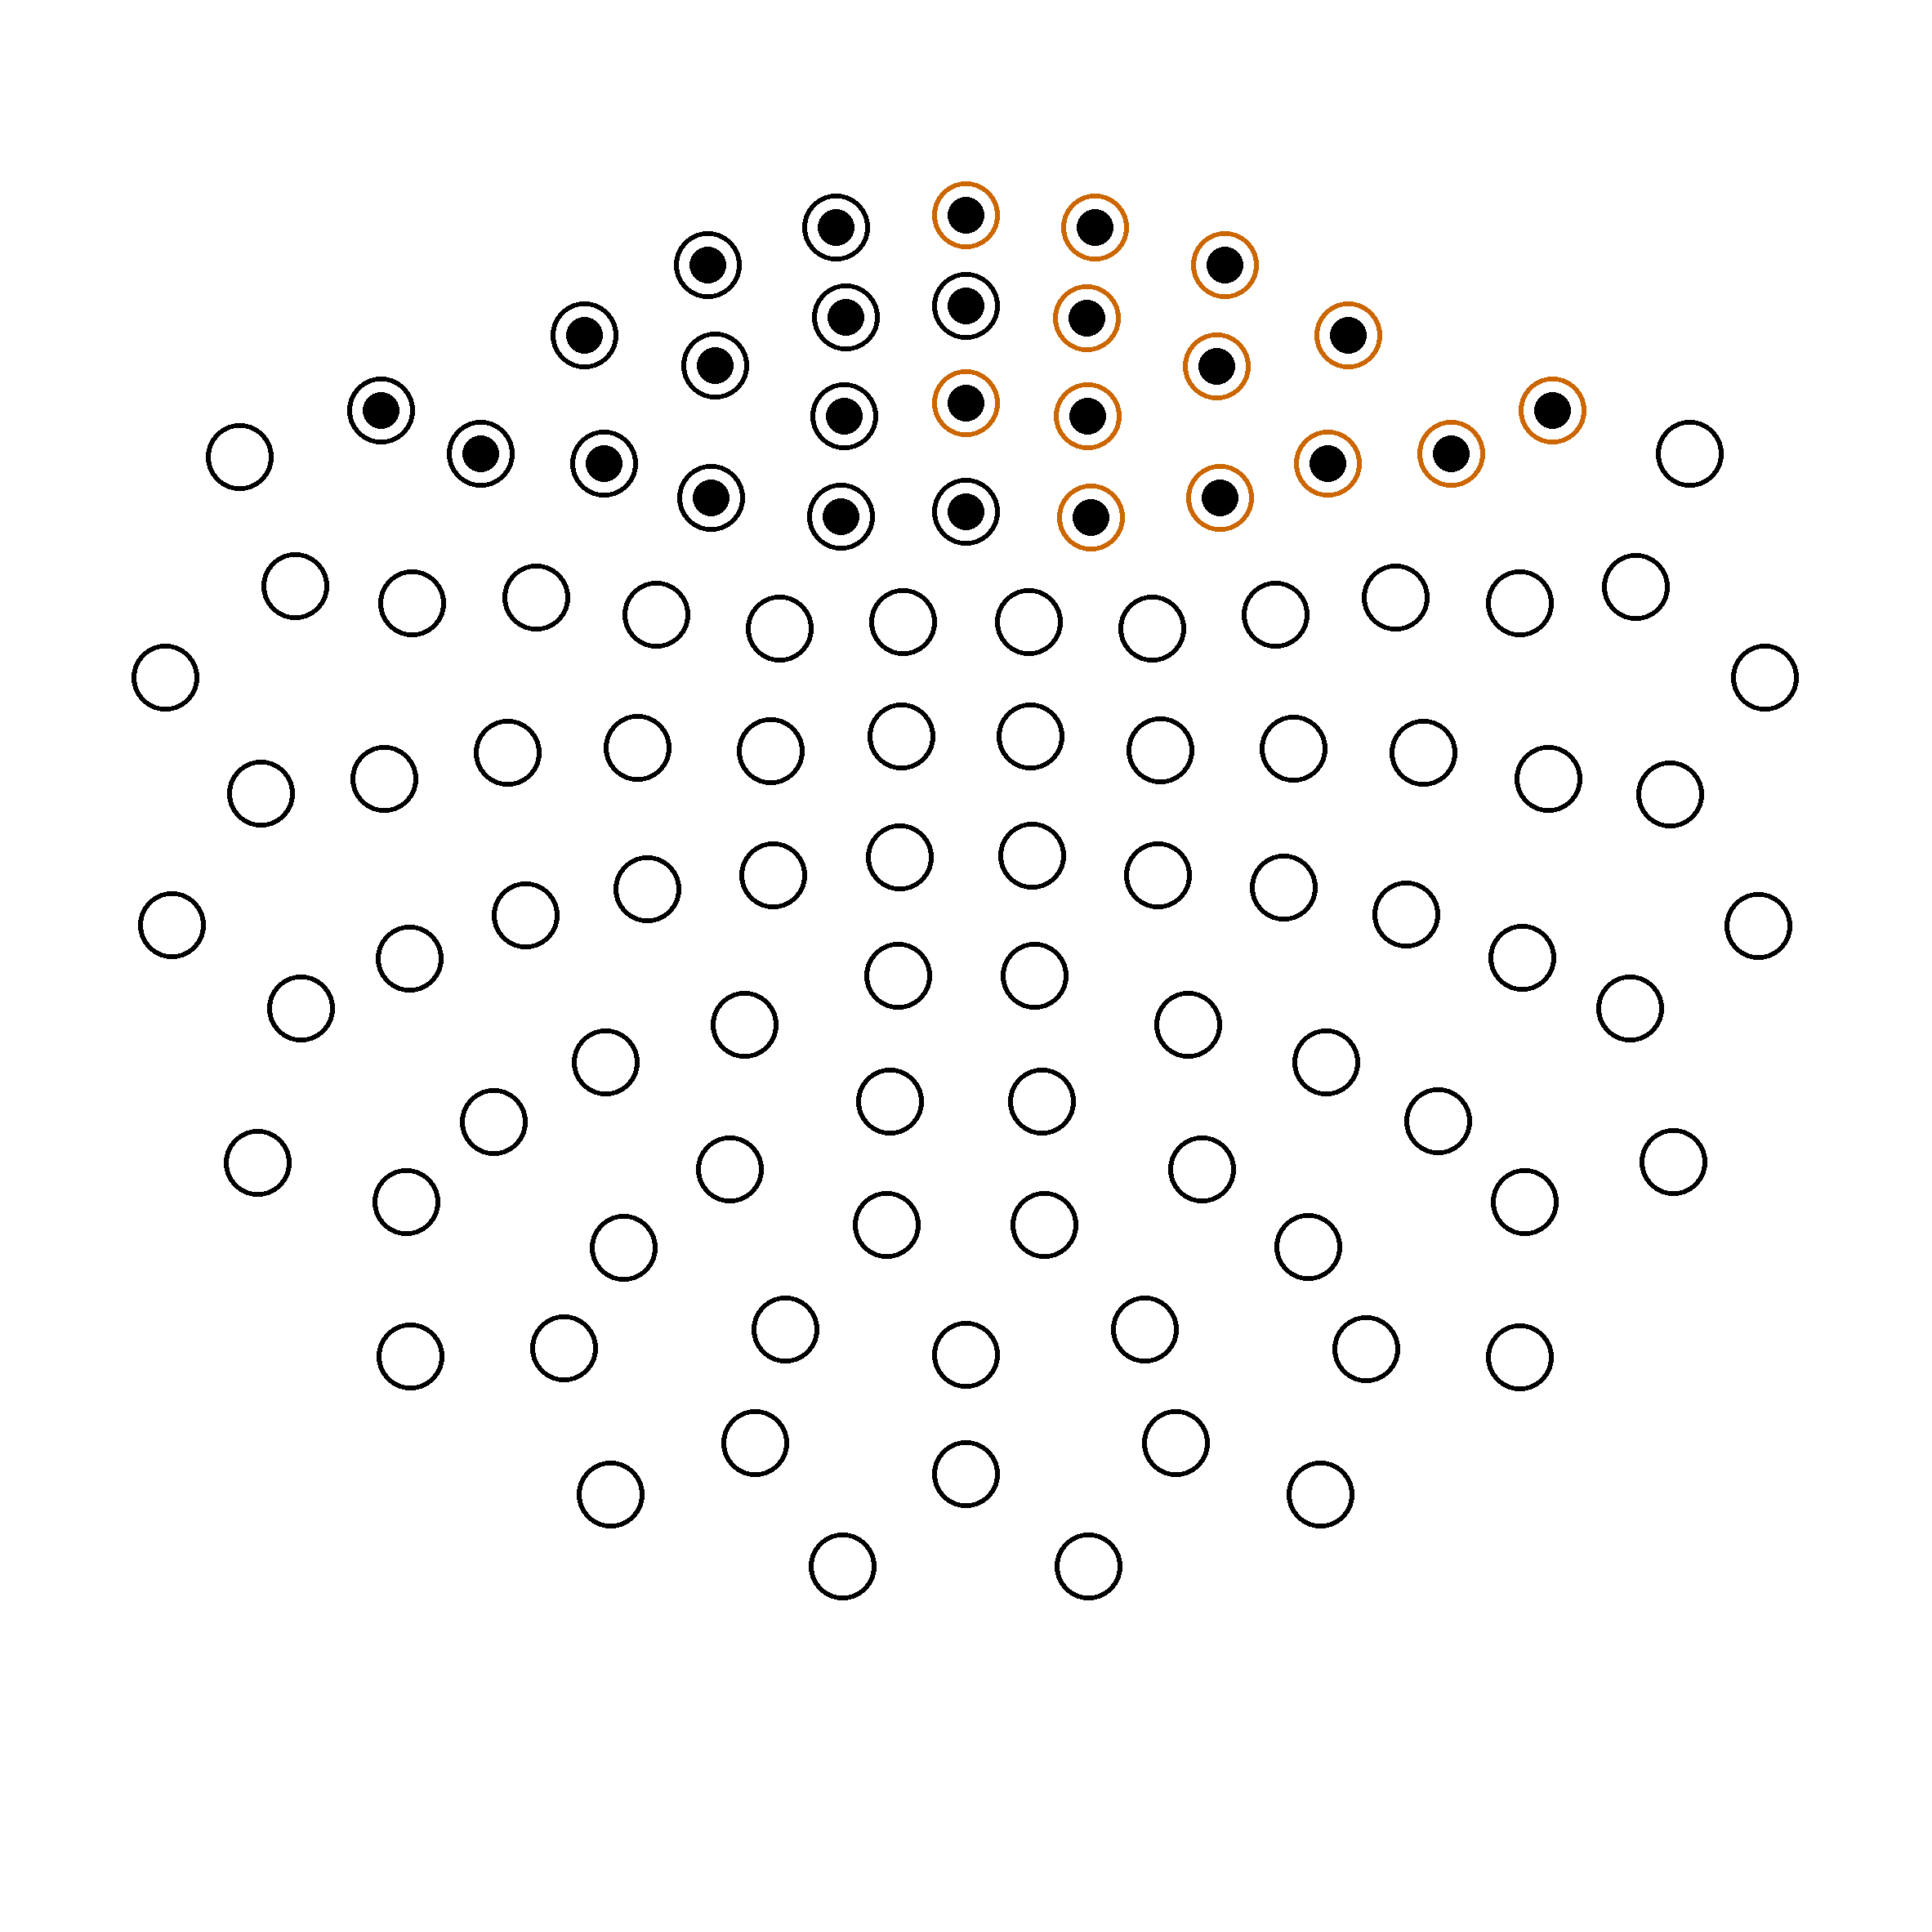
\includegraphics[width=0.24\textwidth]{pics/3_3_frontal_sensors}
\caption{\label{3.3.sensors} Selected channels for each sensor location. From left to right: occipital, parietal, temporal, frontal. The right hemisphere (in red) is also depicted on the right side in each illustration.}
\end{center}
\end{figure}

\subsection{Source space activity}

\paragraph{Anatomical preprocessing}
Cortical reconstruction and volumetric segmentation was performed with the Freesurfer image analysis suite, which is documented and freely available for download online (http://surfer.nmr.mgh.harvard.edu/).
The technical details of these procedures are described in prior publications (Dale et al., 1999; Dale and Sereno, 1993; Fischl and Dale, 2000; Fischl et al., 2001; Fischl et al., 2002; Fischl et al., 2004a; Fischl et al., 1999a; Fischl et al., 1999b; Fischl et al., 2004b; Han et al., 2006; Jovicich et al., 2006; Segonne et al., 2004, Reuter et al. 2010, Reuter et al. 2012).
I followed the recommended processing pipeline ("'recon-all"'), with three optional functions.

First, the option "'-nuintensitycor-3T"' improved brain segmentation accuracy by optimizing the bias field correction \cite{3.3.nuintensity}.

Second, by invoking "'-notal-check"', I skipped the Talairach registration checks.
Talairach registration was prone to failure especially in the infant subjects, and uneccessary for our further processing steps.

Third, I supplied and included T2-weighted MRI datasets with the options "'-T2"' and "'-T2pial"'.
The combination of T1- and T2-weighted images improves tissue differentiation especially around the pia mater, yielding a more accurate cortex segmentation.
This pipeline yielded a continuous, antomically plausible cortical surface in MRI space.


\paragraph{Forward and inverse operator}
For the forward operator, three components were necessary: a source model, a BEM model and a coregistration file.

The cortical surface from Freesurfer was used to construct the source model.
Sources were generated by the MNE function $mne\_setup\_bem$.
The result were 20484 sources (10242 per hemisphere), distributed with approximately equal density over the cortical surface.

The head surface from Freesurfer was used to extract a scalp surface layer.
The BEM was constructed from this scalp layer with the function $mne\_surf2bem$, using the default options.
This function sampled down the original surface to the 4th subdivision of an icosahedron.
The finished BEM consisted of 5140 nodes.

Finally, a coregistration file provided the transformation between MRI space and MEG space.
This coregistration attempted to minimize the distance between digitized head surface points and the head surface extracted from the MRI. 
It was performed for each subject individually using the software $mne\_analyze$.
The initial fit was done manually, with visual error feedback.
The following fine adjustment was performed automatically.
This process was repeated until the average spatial error was less than 2mm.
These three components were assembled into a forward operator by the method $mne\_do\_forward\_solution()$.


For the inverse operator, three components were necessary: the forward model, a noise covariance matrix, and a regularization factor.
Each component was calculated individually for each subject.

The first component, the forward model, was supplied by the previous step.

For the second component, the noise covariance matrix, the 1000ms after visual onset were extracted from each trial.
Then, the covariance matrix was computed from this data with the function $mne.compute\_covariance()$.

The third component, the regularization factor was determined from this noise covariance matrix.
First, only coefficients from gradiometer channels were selected.
Second, these coefficients were transformed with a singular value decomposition.
Third, the upper cutoff was defined as the first value of the transformed coefficients.
Fourth, the index at which the transformed coefficients performed the steepest drop in logarithmic value was determined.
Fifth, this index was defined as the maximum amount of usable dimensions.
Sixth, the lower cutoff was defined as the value at this index, plus 15\%.
Seventh, the regularization factor was computed by dividing the lower cutoff by the higher cutoff.


The inverse operator was computed from these three components by the method \linebreak $mne\_do\_inverse\_operator()$. The regularization factor was supplied with the option \linebreak "'--megreg"'.

\paragraph{Inverse solution}
For determining regional cortical activity, 8 regions needed to be defined: the primary auditory cortex (PAC), the anterior and posterior parts of the superior temporal sulcus (a/pSTS), the anterior and posterior parts of the superior temporal gyrus (a/pSTG), Brodmann area 45 (BA45), Brodmann area 44 (BA44) and the ventral Brodmann area 6 (BA6v).
The regions were spatially defined manually on the cortex of the reference subject.
Freesurfer provided the aparc.a2009s segmentation, which became the basis for this regional selection.
The final regions of interest on the reference brain are visualized in Fig. \ref{3.3.ROI}.
These regions were automatically mapped from the reference cortex onto the cortices of all other subjects during the next step.

\begin{figure}[h]
\begin{center}
\vspace{7mm}
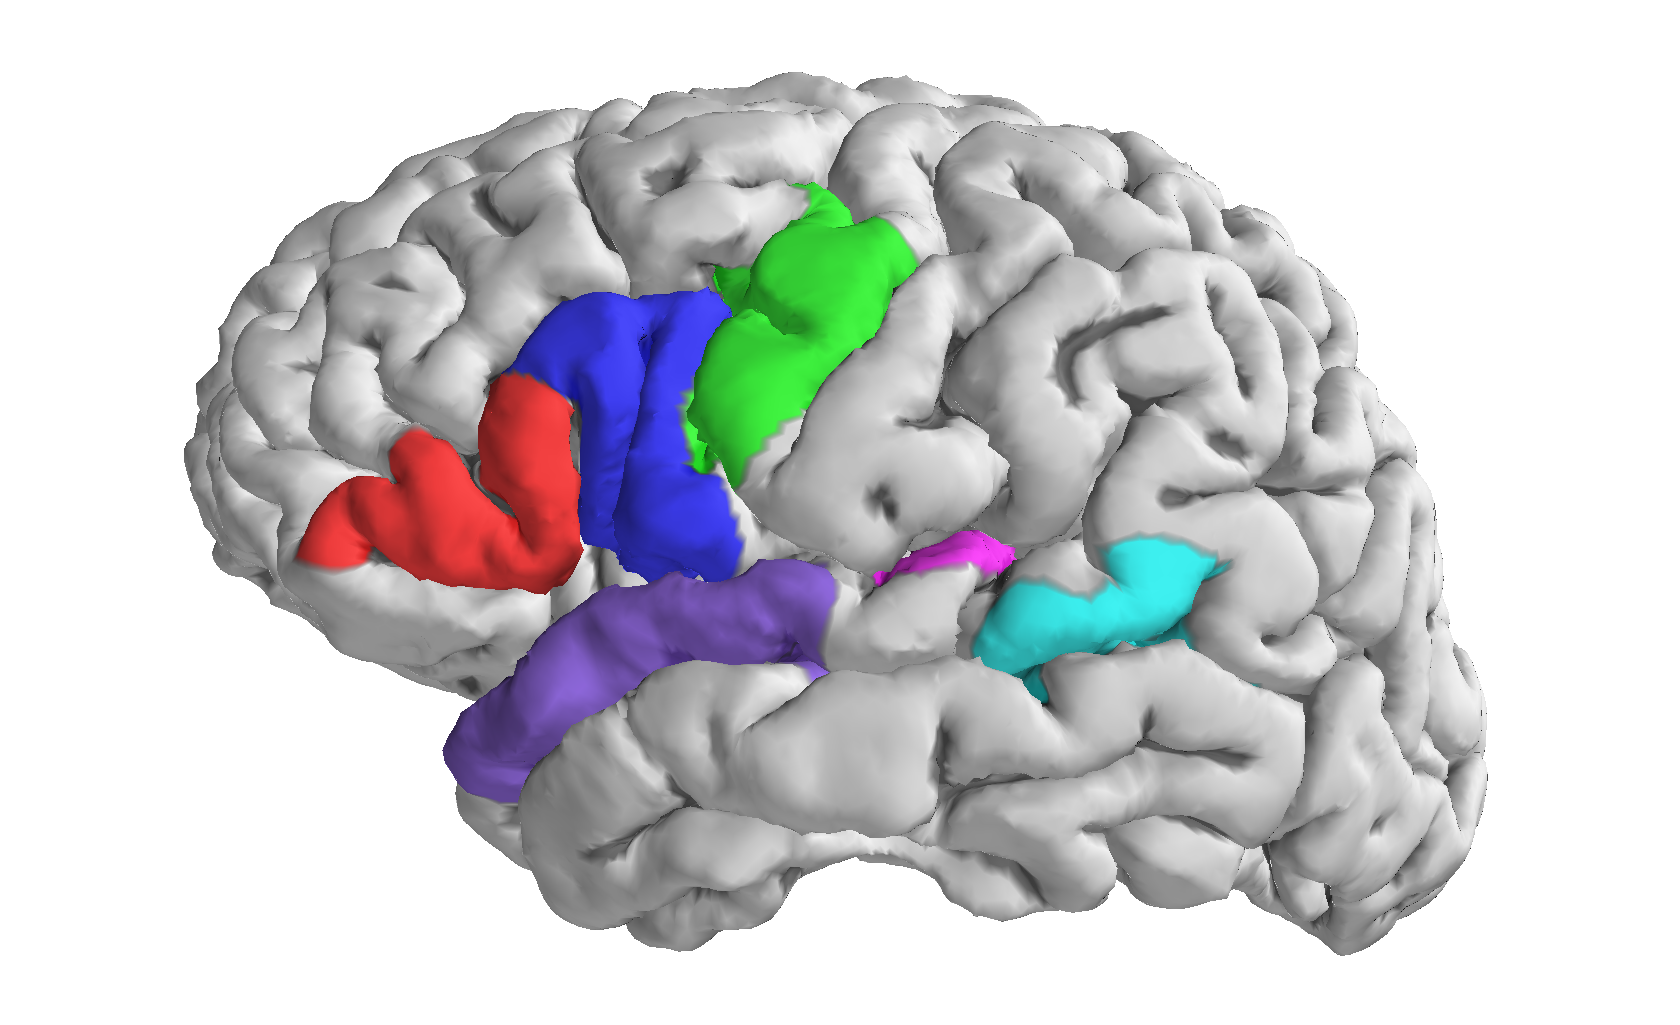
\includegraphics[width=0.49\textwidth]{pics/dh55a-pial-lh}
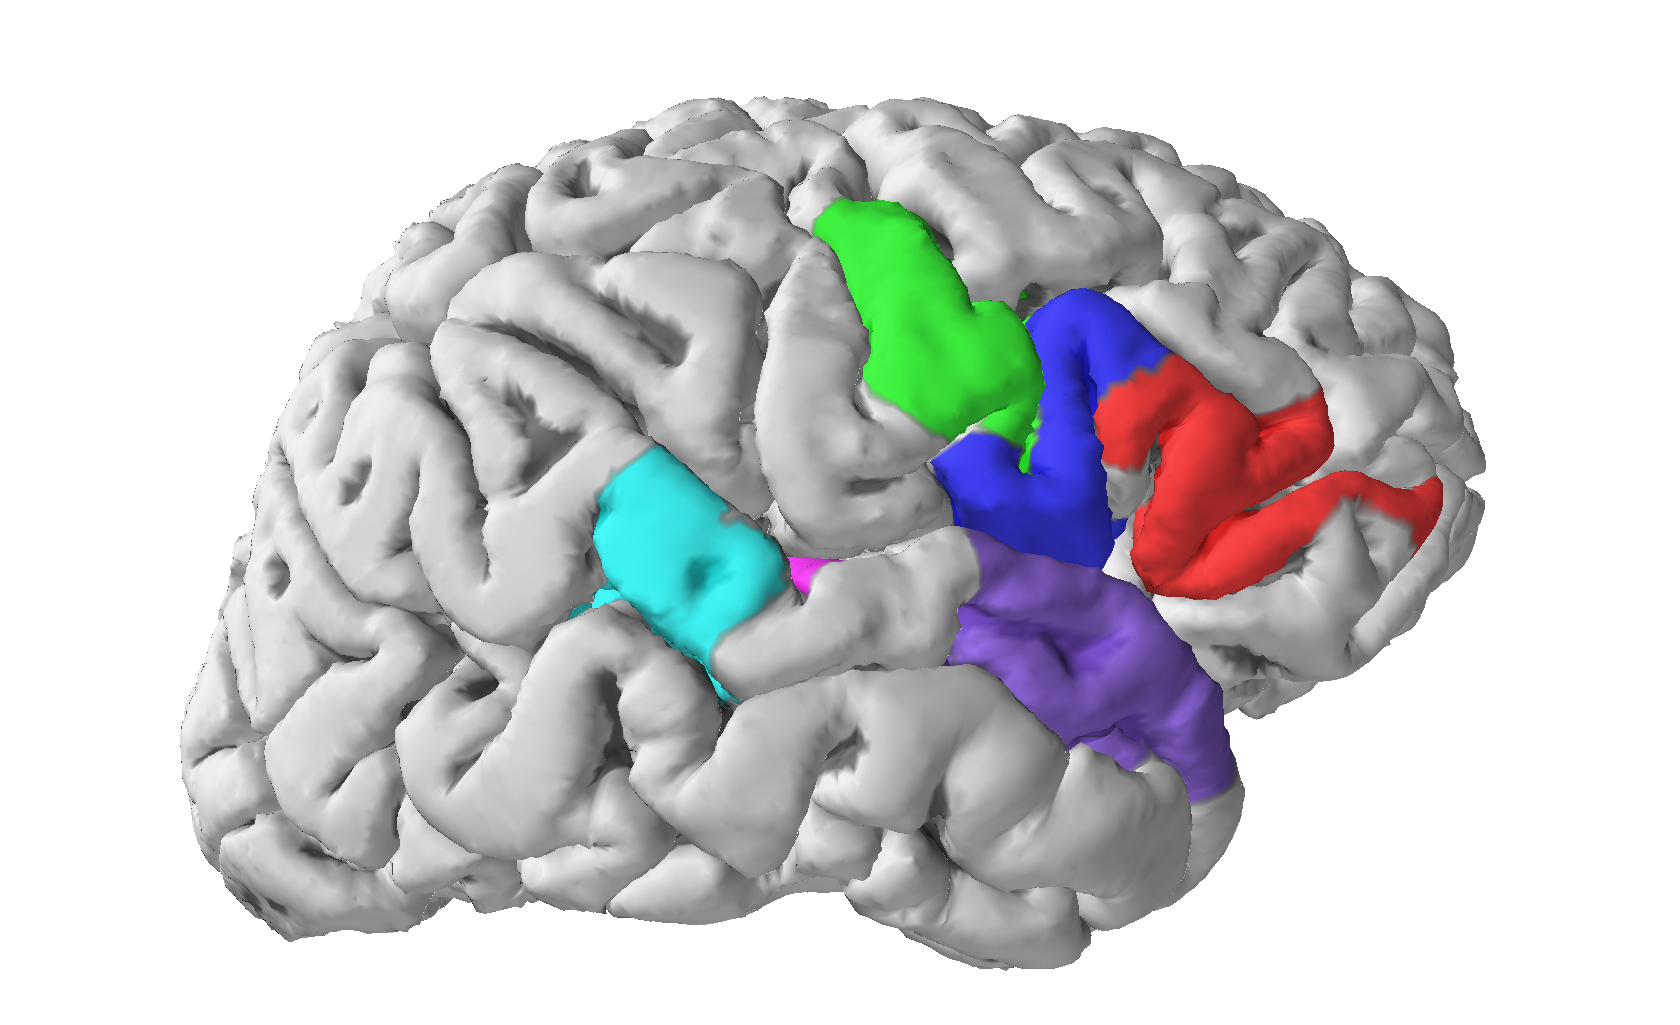
\includegraphics[width=0.49\textwidth]{pics/dh55a-pial-rh}
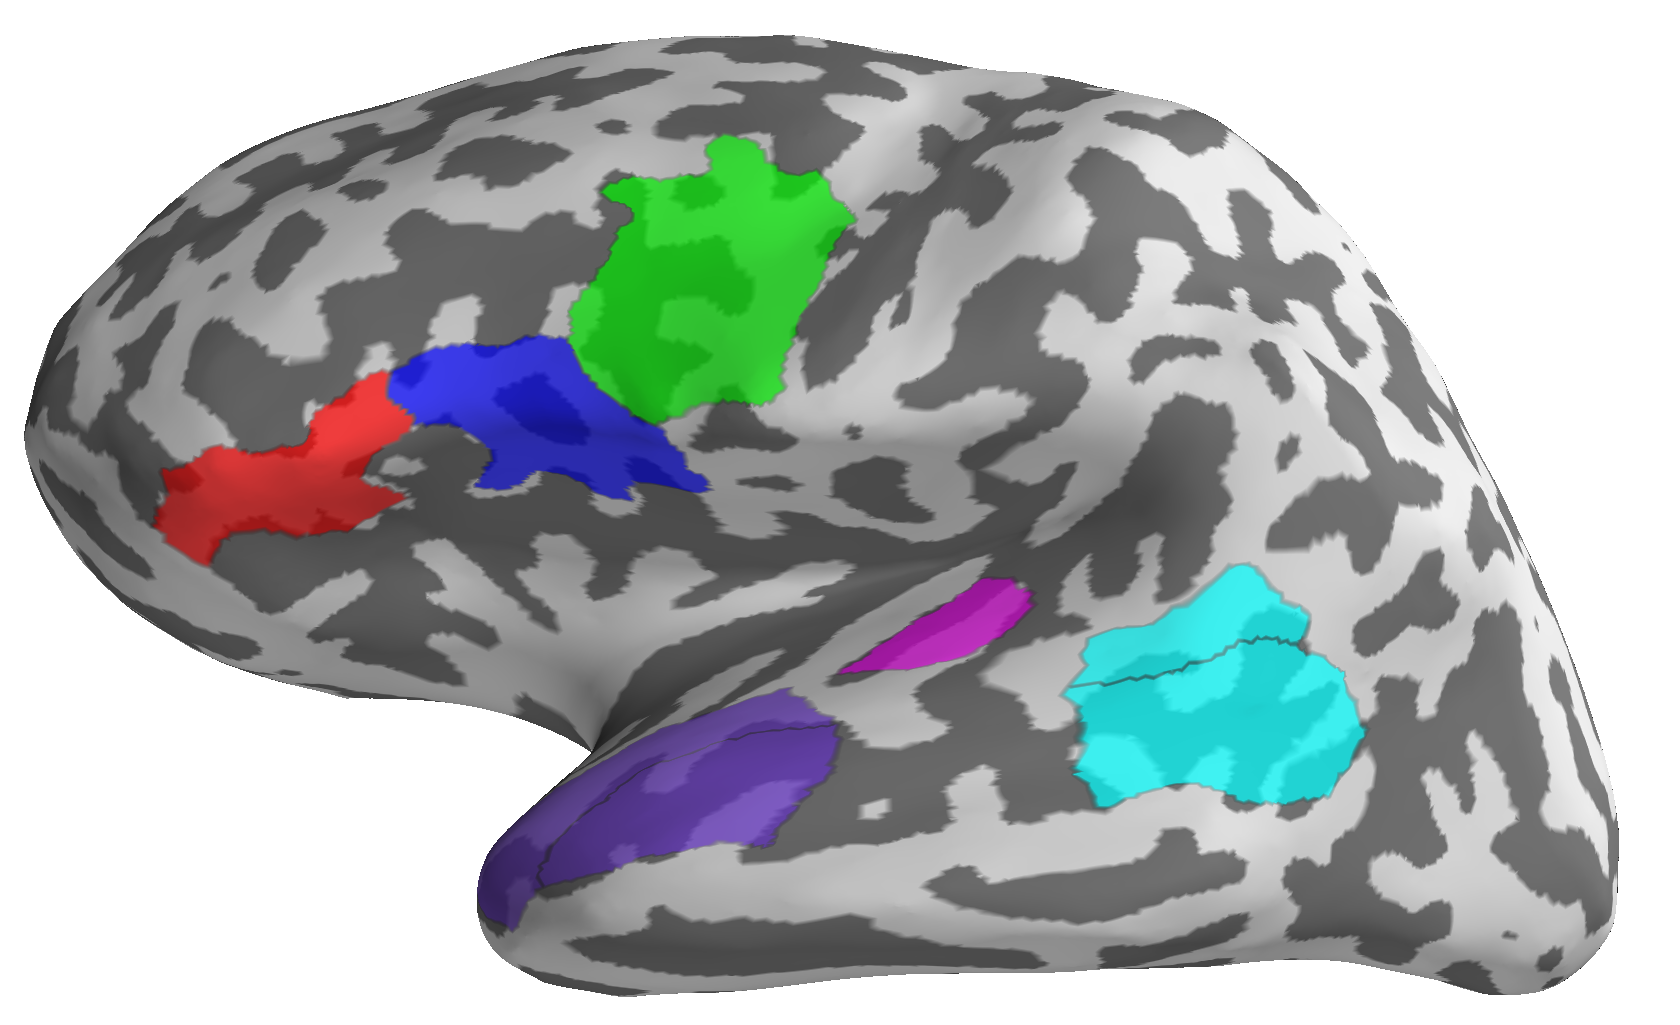
\includegraphics[width=0.49\textwidth]{pics/dh55a-inflated-lh}
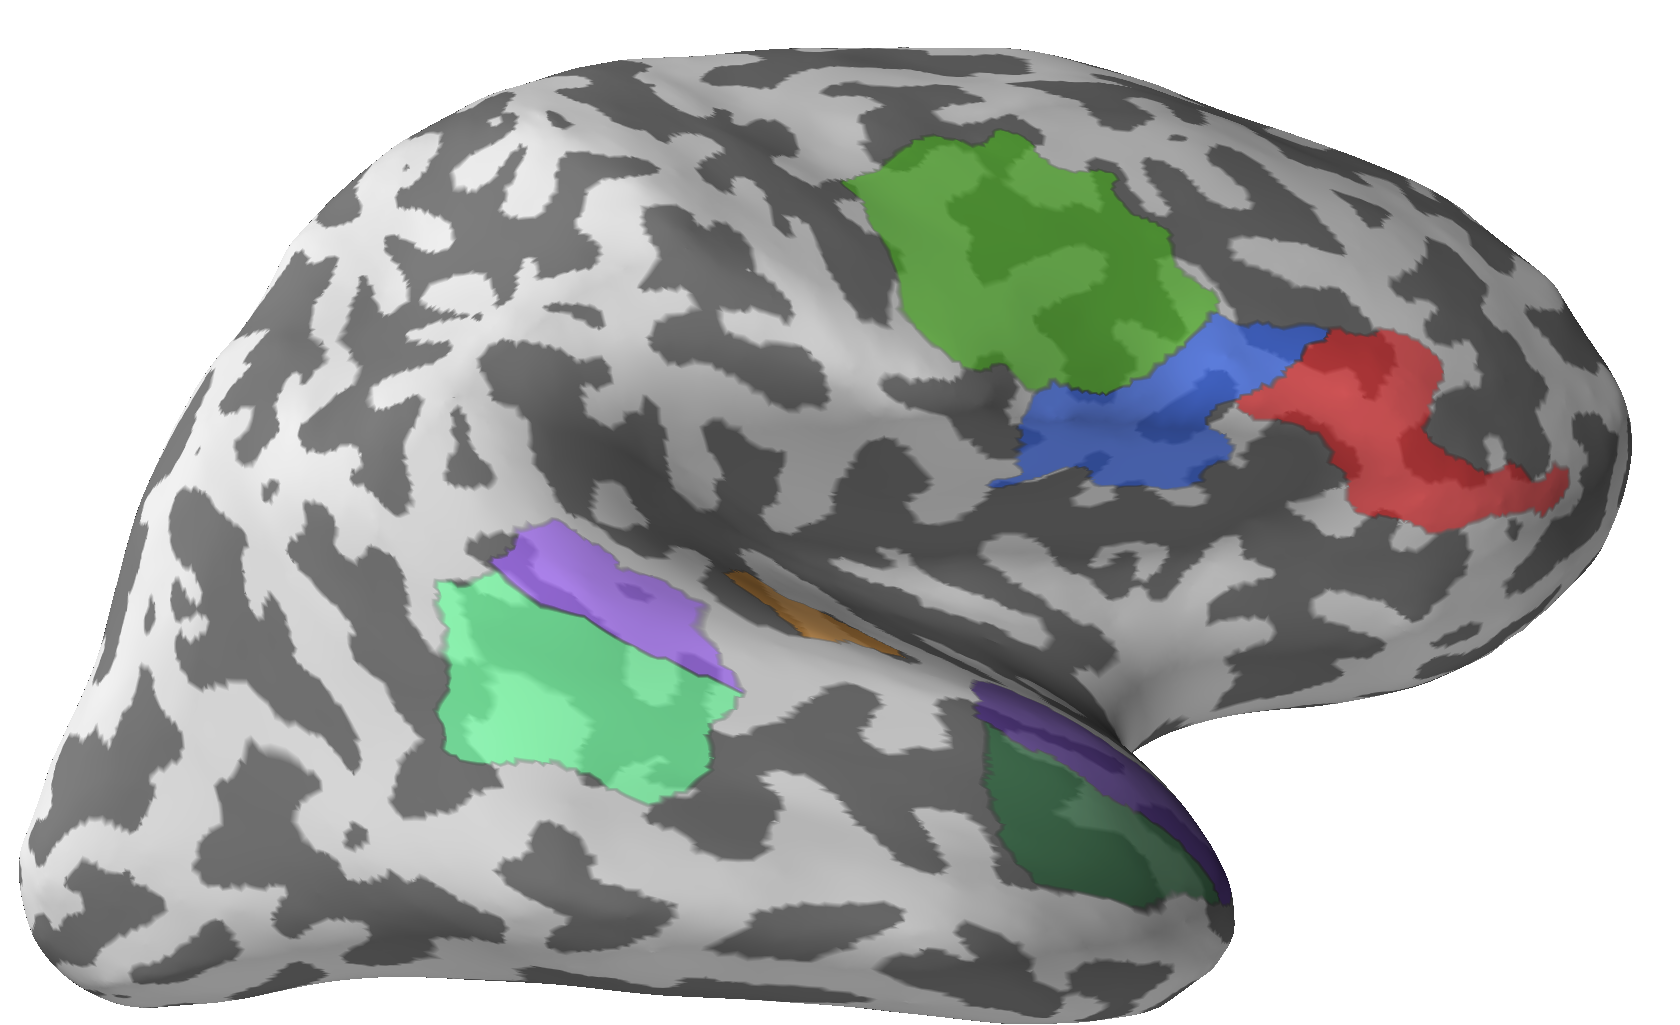
\includegraphics[width=0.49\textwidth]{pics/dh55a-inflated-rh}
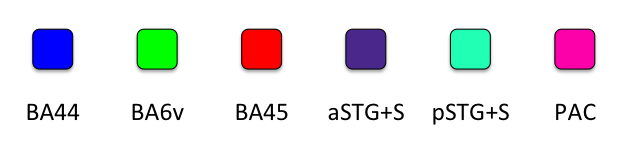
\includegraphics[width=0.75\textwidth]{pics/3_3_ROIlegend}
\caption{\label{3.3.ROI} Selected regions of interest on the reference brain. Top: selected regions on the folded cortex. Bottom: selected regions on the inflated cortex.}
\end{center}
\end{figure}

The inverse operator was then used to calculate inverse solutions from MEG sensor data.
Inverse solutions were calculated for each time point, region, trial and subject individually.
The process was performed by the function $mne.minimum\_norm.apply\_inverse\_epochs()$, with sLORETA as the inverse method.
The option "'pick\_ori=normal"' ensured that currents leaving and entering the cortex were designated positive and negative, respectively.
Due to the combination of passive and active noise reduction and artifact suppression, I assumed a fairly high signal-to-noise-ratio (SNR) of 100:1 for each individual source.
The regularization factor was estimated by $\frac{1}{SNR} = 10^{-4}$.
The result was a series of activation patterns within each region.
Finally, the mean of regional node activity was calculated for each time point, region, trial and subject.


The resulting localized activity was again subjected to a cluster analysis.
Extracted trials were split into a 4 parts (2 groups x 2 conditions).
The two groups were evaluated separately.
Trials contained average data from six regions (PAC, aSTS+G, pSTS+G, BA44, BA45 and BA6v).
Clusters were determined with the MNE function $stats.permutation\_cluster\_test()$ \cite{3.3.clustertest}.
The function was run with 2500 permutations, and an t-threshold of 2.0.

For visualization purposes, grand average activity was calculated for each cortical region, group and condition.


% \subsection{Interaction analysis}

% The TRENtool software was used for exploring transfered entropy between cortical areas.
% - Role of embedding, Ragwitz optimization
% - statistical tests between conditions and multiple comparisons



\chapter{Results}\label{results}

\section{Behavioral results}

If not noted otherwise, two comma-separated values in brackets describe the upper and lower values of a 95\% confidence interval.

\subsection{Response times}

A Shapiro-Wilk test was conducted to determine if individual response times were normal distributed.
All subjects failed this test (p < 0.001), indicating a strong deviation from normality.
Therefore, I represented individual response times by their median.

Children needed a median time of 1.91s (1.64s, 2.19s) to respond to object-relative clauses.
For subject-relative clauses, they needed 1.97s (1.69s, 2.25s).
Adults needed a median time of 1.51s (1.28s, 1.73s) to respond to object-relative clauses.
For subject-relative clauses, they needed 1.60s (1.37s, 1.82s).

A Shapiro-Wilk test determined that response time data was normal distributed with a probability between 1.5\% and 27\%.
A Levene's test determined that the probability of median response times being normal distributed was ?\%.
Supported by these findings, the response times were included into the ANOVA.

\subsection{Response accuracy}

For the analysis of variance (ANOVA), all data must be normal distributed with equal variance.
A Shapiro-Wilk test determined that the probability of accuracy data being normal distributed was between 2.0 and 20.3\%.
A Levene's test yielded that the probability that accuracy data were distributed with equal variance was less than p = 0.1\%.

The ANOVA is known to be robust for considerable deviations from the normal distribution.
However, it is highly vulnerable to violation the assumption of equal variances.
To meet this requirement, I transformed the accuracy data with the inverse sigmoid function.
This procedure, however, created singularities in some extreme cases, i.e., when a subject performed with a 100\% accuracy rate.
To prevent this issue, I added a single incorrect trial to every subject's performance for the following analysis.

After the transformation, the same tests as before were conducted.
The probability for transformed accuracy data being normal distributed was between 0.5\% and 27\%.
The probability for transformed accuracy data being distributed with equal variance was p = 72.2\%.
Supported by these findings, the transformed accuracy data was included in the ANOVA.

\subsection{Analysis of combined performance data}

Two ANOVA were conducted with the transformed accuracy data and the median response times.
Each subject provided one data point for each metric.
Data were analyzed with a group x condition design.
Accuracy estimates were transformed back with the sigmoid function $r = \frac{1}{1+e^{\hat{-r}}}$.

Children responded 0.39s slower than adults (1.94s vs. 1.55s).
This difference was significant ($F_{56} = 9.4$, $p = 0.3\%$).

Children responded with an average accuracy of 93.8\% (92.2\%, 95.0\%).
Adults performed much better, with an average accuracy of 97.9\% (97.5\%, 98.3\%).
This difference was highly significant ($F_{56} = 52$, $p = 1.6*10^{-9}$).

Sentence condition had no impact on median response times ($F = 0.33$, $p = 57\%$) or on response accuracy ($F = 1.3$, $p = 26\%$).
There was no interaction effect between group and sentence condition ($F < 0.1$, $p > 80\%$).

\section{Sensor-space activity}

We computed average event-related fields (ERF) for each subject and sensor region.
Activity from these ERF was selected with two different types of time windows.

A positive effect indicates that activity evoked by object-relative clauses was polarized more positively than activity evoked by subject-relative clauses. In the case of gradiometers, "'more positive"' means a higher regional RMS. With localized data, "'more positive"' means a higher z-score from the sLORETA source reconstruction.


\subsection{Interval analysis}
For this analysis, sensor activity from separate regions and hemispheres was compared blindly between 0 and 2200ms after onset in 200ms intervals.

After FDR-correction for 10 comparisons, no sensor region showed any non-spurious effect in either group ($p > 3\%$).

\subsection{Cluster analysis}
For this analysis, activity was compared between conditions using a temporal cluster analysis.

For children, significant differences were observed in the following sensor groups:
Right parietal magnetometers showed a negative effect between 159ms and 374ms ($p = 1.4\%$).
Left frontal magnetometers showed a negative effect between 375ms and 666ms ($p = 1.8\%$).
Left temporal magnetometers showed a negative effect between 349ms and 627ms ($p = 0.8\%$).
Right temporal gradiometers showed a positive effect between 1384ms and 1663ms ($p = 3.8\%$).

\begin{figure}[!h]
\begin{center}
\includegraphics[width=0.49\textwidth]{pics/children_Left-frontal-magnetometer.png}
\includegraphics[width=0.49\textwidth]{pics/children_Right-frontal-magnetometer.png}
\includegraphics[width=0.49\textwidth]{pics/children_Left-frontal-gradiometer.png}
\includegraphics[width=0.49\textwidth]{pics/children_Right-frontal-gradiometer.png}
\includegraphics[width=0.49\textwidth]{pics/kids_Left-frontal_mag.png}
\includegraphics[width=0.49\textwidth]{pics/kids_Right-frontal_mag.png}
\includegraphics[width=0.49\textwidth]{pics/kids_Left-frontal_grad.png}
\includegraphics[width=0.49\textwidth]{pics/kids_Right-frontal_grad.png}
\caption{\label{4.2.activity.kids.frontal} Combined frontal sensor activity from children in separate sensor groups. Top row: magnetometer activity; middle row: gradiometer activity; bottom two rows: equivalent results from the cluster analysis. Charts on the left side depict activity from the left hemisphere and vice versa.}
\end{center}
\end{figure}


\begin{figure}[!h]
\begin{center}
\includegraphics[width=0.49\textwidth]{pics/children_Left-temporal-magnetometer.png}
\includegraphics[width=0.49\textwidth]{pics/children_Right-temporal-magnetometer.png}
\includegraphics[width=0.49\textwidth]{pics/children_Left-temporal-gradiometer.png}
\includegraphics[width=0.49\textwidth]{pics/children_Right-temporal-gradiometer.png}
\includegraphics[width=0.49\textwidth]{pics/kids_Left-temporal_mag.png}
\includegraphics[width=0.49\textwidth]{pics/kids_Right-temporal_mag.png}
\includegraphics[width=0.49\textwidth]{pics/kids_Left-temporal_grad.png}
\includegraphics[width=0.49\textwidth]{pics/kids_Right-temporal_grad.png}
\caption{\label{4.2.activity.kids.temporal} Combined temporal sensor activity from children in separate sensor groups. Top row: magnetometer activity; middle row: gradiometer activity; bottom two rows: equivalent results from the cluster analysis. Charts on the left side depict activity from the left hemisphere and vice versa.}
\end{center}
\end{figure}


\begin{figure}[!h]
\begin{center}
\includegraphics[width=0.49\textwidth]{pics/children_Left-parietal-magnetometer.png}
\includegraphics[width=0.49\textwidth]{pics/children_Right-parietal-magnetometer.png}
\includegraphics[width=0.49\textwidth]{pics/children_Left-parietal-gradiometer.png}
\includegraphics[width=0.49\textwidth]{pics/children_Right-parietal-gradiometer.png}
\includegraphics[width=0.49\textwidth]{pics/kids_Left-parietal_mag.png}
\includegraphics[width=0.49\textwidth]{pics/kids_Right-parietal_mag.png}
\includegraphics[width=0.49\textwidth]{pics/kids_Left-parietal_grad.png}
\includegraphics[width=0.49\textwidth]{pics/kids_Right-parietal_grad.png}
\caption{\label{4.2.activity.kids.parietal} Combined parietal sensor activity from children in separate sensor groups. Top row: magnetometer activity; middle row: gradiometer activity; bottom two rows: equivalent results from the cluster analysis. Charts on the left side depict activity from the left hemisphere and vice versa.}
\end{center}
\end{figure}

\clearpage
For adults, clusters of significant differences were observed by left-temporal gradiometers and left-parietal magnetometers.
Left frontal gradiometers showed a weak positive effect between 131ms and 284ms ($p = 6.3\%$).
Left temporal gradiometers showed a positive effect between 257ms and 480ms ($p = 2.1\%$).
Left parietal magnetometers showed a positive effect between 618ms and 765ms ($p = 0.64\%$).
Left temporal magnetometers showed a weak negative effect between 1351 and 1491ms ($p = 8.4\%$).


\begin{figure}[!h]
\begin{center}
\includegraphics[width=0.49\textwidth]{pics/adults_Left-frontal-magnetometer.png}
\includegraphics[width=0.49\textwidth]{pics/adults_Right-frontal-magnetometer.png}
\includegraphics[width=0.49\textwidth]{pics/adults_Left-frontal-gradiometer.png}
\includegraphics[width=0.49\textwidth]{pics/adults_Right-frontal-gradiometer.png}
\includegraphics[width=0.49\textwidth]{pics/adults_Left-frontal_mag.png}
\includegraphics[width=0.49\textwidth]{pics/adults_Right-frontal_mag.png}
\includegraphics[width=0.49\textwidth]{pics/adults_Left-frontal_grad.png}
\includegraphics[width=0.49\textwidth]{pics/adults_Right-frontal_grad.png}
\caption{\label{4.2.activity.adults.frontal} Combined frontal sensor activity from adults in separate sensor groups. Top row: magnetometer activity; middle row: gradiometer activity; bottom two rows: equivalent results from the cluster analysis. Charts on the left side depict activity from the left hemisphere and vice versa.}
\end{center}
\end{figure}


\begin{figure}[!h]
\begin{center}
\includegraphics[width=0.49\textwidth]{pics/adults_Left-temporal-magnetometer.png}
\includegraphics[width=0.49\textwidth]{pics/adults_Right-temporal-magnetometer.png}
\includegraphics[width=0.49\textwidth]{pics/adults_Left-temporal-gradiometer.png}
\includegraphics[width=0.49\textwidth]{pics/adults_Right-temporal-gradiometer.png}
\includegraphics[width=0.49\textwidth]{pics/adults_Left-temporal_mag.png}
\includegraphics[width=0.49\textwidth]{pics/adults_Right-temporal_mag.png}
\includegraphics[width=0.49\textwidth]{pics/adults_Left-temporal_grad.png}
\includegraphics[width=0.49\textwidth]{pics/adults_Right-temporal_grad.png}
\caption{\label{4.2.activity.adults.temporal} Combined temporal sensor activity from adults in separate sensor groups. Top row: magnetometer activity; middle row: gradiometer activity; bottom two rows: equivalent results from the cluster analysis. Charts on the left side depict activity from the left hemisphere and vice versa.}
\end{center}
\end{figure}


\begin{figure}[!h]
\begin{center}
\includegraphics[width=0.49\textwidth]{pics/adults_Left-parietal-magnetometer.png}
\includegraphics[width=0.49\textwidth]{pics/adults_Right-parietal-magnetometer.png}
\includegraphics[width=0.49\textwidth]{pics/adults_Left-parietal-gradiometer.png}
\includegraphics[width=0.49\textwidth]{pics/adults_Right-parietal-gradiometer.png}
\includegraphics[width=0.49\textwidth]{pics/adults_Left-parietal_mag.png}
\includegraphics[width=0.49\textwidth]{pics/adults_Right-parietal_mag.png}
\includegraphics[width=0.49\textwidth]{pics/adults_Left-parietal_grad.png}
\includegraphics[width=0.49\textwidth]{pics/adults_Right-parietal_grad.png}
\caption{\label{4.2.activity.adults.parietal} Combined parietal sensor activity from adults in separate sensor groups. Top row: magnetometer activity; middle row: gradiometer activity; bottom two rows: equivalent results from the cluster analysis. Charts on the left side depict activity from the left hemisphere and vice versa.}
\end{center}
\end{figure}


The generally lower significance levels in adults imply an overall weaker impact of syntactic condition on sensor activity.
Syntactic effects in the left fronto-parietal region occurred earlier in adults (131-480ms) than in children (349-666ms).
Effects were much more lateralized in children, with a weak but distinct support from right parietal and temporal regions.
The strong effect in adults' left parietal regions between 618ms and 765ms is unparalleled in children.
These differences seem to promise a group effect, and will be resolved more accurately in the next section.

\clearpage\section{Source-space activity}\label{4.3}

\subsection{Comparison of means}
Localized activity from eight regions of interest (PAC, aSTS, aSTG, pSTS, pSTG, BA44, BA45 and BA6v) were examined for a syntax effect.
For this purpose, average activity was computed and compared within evenly-spaced time intervals. "'positive"' effects imply elevated activity during object-related clauses, while "'negative"' effects imply elevated activity during subject-related clauses.

\paragraph{Interval analysis}
The interval comparison (0ms to 2200ms) yielded three distinct temporal clusters in adults.

During the first time cluster, 0ms to 200ms, especially the right PAC showed a strong negative effect ($p = 0.5\%$, $t_{17} = -3.7$).
Other negative effects were visible in the left PAC ($p = 3.0\%$, $t_{17} = -2.9$) and the left BA45 ($p = 5.1\%$, $t_{17} = -2.6$).

The second time cluster, 400ms to 800ms, was signified by simultaneous effects in seven regions.
Both left and right PAC showed a positive effect ($p = 3.0\%$ and $p < 0.1\%$, $t_{17} = 2.9$ and $t_{17} = 4.8$).
The right pSTG showed negative effects, which grew more noticable during the progression of the time cluster.
In the first half of the cluster (400ms to 600ms), the condition effect started very weakly ($p = 7.9\%$, $t_{17} = -2.4$).
During the second half of the cluster (600ms to 800ms), the effect strengthened noticably ($p = 1.0\%$, $t_{17} = -3.9$).
The left aSTG showed a similar pattern: weak negative effect between 400ms and 600ms ($p = 2.1\%$, $t_{17} = -3.2$), which became noticably more distinct between 600ms and 800ms ($p = 0.4\%$, $t_{17} = -4.3$).
The left BA45 showed a constant and strong positive activation effect ($p = 0.6\%$, $t_{17} = 3.9$).
Otherwise, very weak positive effects ($p < 7\%$, $t_{17} = 3.0$) could be observed in the left BA6v (400ms to 600ms) and the left BA44 (600ms to 800ms).

The third time cluster, 1000ms to 1600ms, only showed effects in three regions.
The right PAC showed a very late, distinctly negative effect ($p = 0.9\%$, $t_{17} = -3.3$, between 1400ms and 1600ms).
Very weak positive effects ($p < 8\%$, $t_{17} = 2.4$) were observed in the right pSTG (1000ms to 1200ms) and the left aSTG (1400ms to 1600ms).
At the same time (1400ms to 1600ms), the left aSTS showed a very weak effect as well, but with opposite polarity ($p = 6.6\%$, $t_{17} = -3.0$).

\begin{figure}[h]
\begin{center}
\includegraphics[width=0.49\textwidth]{pics/signed-adults-PAC-lh.png}
\includegraphics[width=0.49\textwidth]{pics/signed-adults-PAC-rh.png}
\includegraphics[width=0.49\textwidth]{pics/signed-adults-aSTS-lh.png}
\includegraphics[width=0.49\textwidth]{pics/signed-adults-aSTS-rh.png}
\includegraphics[width=0.49\textwidth]{pics/signed-adults-aSTG-lh.png}
\includegraphics[width=0.49\textwidth]{pics/signed-adults-aSTG-rh.png}
\includegraphics[width=0.49\textwidth]{pics/signed-adults-BA45-lh.png}
\includegraphics[width=0.49\textwidth]{pics/signed-adults-BA45-rh.png}
\caption{\label{4.3.activity.adults.ventral} Combined activity from adults in separate cortical regions. Top row: PAC; second row: aSTS; third row: aSTG; bottom row: BA45. Charts on the left side depict activity from the left hemisphere and vice versa.}
\end{center}
\end{figure}


\begin{figure}[h]
\begin{center}
\includegraphics[width=0.49\textwidth]{pics/signed-adults-BA6v-lh.png}
\includegraphics[width=0.49\textwidth]{pics/signed-adults-BA6v-rh.png}
\includegraphics[width=0.49\textwidth]{pics/signed-adults-pSTS-lh.png}
\includegraphics[width=0.49\textwidth]{pics/signed-adults-pSTS-rh.png}
\includegraphics[width=0.49\textwidth]{pics/signed-adults-pSTG-lh.png}
\includegraphics[width=0.49\textwidth]{pics/signed-adults-pSTG-rh.png}
\includegraphics[width=0.49\textwidth]{pics/signed-adults-BA44-lh.png}
\includegraphics[width=0.49\textwidth]{pics/signed-adults-BA44-rh.png}
\caption{\label{4.3.activity.adults.ventral} Combined activity from adults in separate cortical regions. Top row: BA6v; second row: pSTS; third row: pSTG; bottom row: BA44. Charts on the left side depict activity from the left hemisphere and vice versa.}
\end{center}
\end{figure}

\clearpage

The interval analysis yielded no non-spurious effects ($p > 5\%$) from children.
This fact prompted a more extensive investigation.

\subsection{Post-hoc analysis}

Compared to the sensor-space analysis, source-space data yielded much more pronounced effects in adults.
Since this effect differentiation was the main goal of the localization process, these results were in line with my expectations.
However, localization of cortical activity in children failed to yield a similar improvement.
The localization procedure was identical for both groups, so no procedural difference could have affected the results.

That left two major possibilities for these unexpected results.

\paragraph{Possible explanations}
First, the localization process may have produced drastically worse inverse solutions for children than for adults.
Due to the hands-off approach of the generation of cortical surfaces, there are no parameters for the transfer of regional boundaries between the (adult) reference brain and each infant brain.
This automated process could have resulted in a systematically higher spatial error between my regional definitions and the actual functional regions in infants than in adults.
Less realistic regional definitions in children than in adults can result in unintended overlap between functional regions, and lead to a diminished experimental effect in each region.
It is also be possible that the automated segmentation process, that Freesurfer uses for extracting the cortex surface, is not optimized for infant brains.
An imprecise definition of the cortical surface would result in a skewed spatial location of the source dipoles, again causing regional overlapping and diminishing the experimental effect.
If the localization performed drastically worse for children, the extraction of relevant time intervals and regional connections from the conditional effect would be impossible.

Second, it is possible that the cognitive strategies were stable within each subject, but the strategies of my young subjects were more diverse than those of my adults.
Both cluster analysis and interval analysis are based on the assumption that all subjects in one group use the same cognitive strategy, and the same anatomical pathways.
If this suspicion was true for adults, but not for children, different processing strategies could cancel each other out and produce no effect.
Both the average localized activity and pooled single trials would be vulnerable to this violation.

Third, it is possible that cognitive strategies and pathways vary within individual children, but stay stable within individual adults.
This circumstance would lead the conditional effect to appear in different regions over the course of the task.
Mean regional activity would be blurred because the stationarity assumption would be violated, and the overall effect would be greatly diminshed.

\paragraph{Exploring the explanations}
Unfortunately, in order to compare the first possibility, a ground truth for the dipole locations and activations would be necessary.
This type of reference data is only available in phantom models, therefore the first possibility remains elusive for direct statistical tests.
However, since neither set of localization software was designed for processing infant brains, this possibility remains the default explanation.

To decide whether the second possibility was responsible for the skewed results, I conducted two tests:
First, if the cognitive processes were much more varied in children than in adults, this circumstance should be reflected in a more homogenuous evoked activity within the adults.
To test this hypothesis, I calculated the individual deviation from the group-average activity and compared deviations between both groups.

Second, if the cognitive strategy was less stable in children than in adults, localized activity in children should show more intra-subject variation.
To test this hypothesis, I calculated the individual deviation from the individual-average activity and compared deviations between both groups.

\paragraph{Post-hoc test results}
For the first test, localized pooled activity (evoked by object-relative clauses) was selected from the time window 0ms to 2200ms.
The mean activity was computed from this selected activity from all subjects within each group.
The difference between individual and mean activity was then computed for each cortical region, yielding a time series.
Each time series was reduced to a single value by computing the variance over time.
Variances from both groups were tested for systematic differences with Welch's test.
The Welch test doesn't assume equal variances and allows for unequal sample sizes.
It was implemented in Python with the function \emph{scipy.stats.ttest\_ind()}.
Variances from both groups differed only weakly ($p \approx 5\%$, $t \approx -2.8$) after FDR correction with 8 comparisons.
There was a considerable bias in six regions (all expect for pSTS and pSTG) towards higher group-level variances in adults.
This finding weakened the second possibility (stronger inter-subject variation in children), and indirectly supported the first possibility (better localization in adults).

The second test was based on the same data set as the first test.
Reference activity was calculated by computing the mean of all trials from one subject.
Then, the difference between single trials and the reference trial were computed and reduced by calculating the variance over time.
A single value for each subject was determined by computing the mean of all subject-specific variances.
Again, Welch's test compared individual variance scores between both groups.
The FDR-corrected results (8 comparisons) yielded no significant ($p > 50\%$, $t \approx -1.0$) differences.
This finding weakened the third possibility (stronger intra-subject variation in children), and indirectly supported the first possibility (better localization in adults).

\paragraph{Conclusion}
The deterioration of the syntactical effect in children before and after the source localization can not be explained by a wider spectrum of cognitive strategies.
If anything, adults showed a wider, not a smaller variety of localized activity than children.
By the refutation of the second and third possibilities, the first assumption was strengthened in comparison.
Therefore, it seems as if the inverse solution for childrens' cortical activity failed to match the accuracy of the adults'.
Without the spatio-temporal distribution of condition effects in children, the task of determining the equivalent TOI and ROI showed little promise.
Since accurate TOI and ROI were necessary for the next step, I continued the analysis only with the adult subject group.\section{Source-space interactions}

Transfer entropy was examined across 9 possible functional connections for five time intervals, spanning an interaction delay between 1ms and 50ms.
Time intervals (relative to stimulus onset) are abbreviated with T1 (0ms - 200ms), T2 (200ms - 400ms), T3 (400ms - 600ms), T4 (600ms - 800ms) and T5 (800ms - 1000ms).

First, transfer entropy was compared against surrogate data.
The surrogate test determined whether the transfered entropy (TE) was erroneously detected due to random coincidence.
The effective TE was calculated from the difference between surrogate TE and raw TE.
These values are listed in tables \ref{4.4.TEvalues.a} and \ref{4.4.TEvalues.b}, and visualized in figures \ref{4.4.networkgraph.a} through \ref{4.4.networkgraph.e}. For optimized viewing, I recommend putting pages \pageref{4.4.networkgraph.a} through \pageref{4.4.networkgraph.e} next to each other. 

\vspace{5mm}
\begin{table}[h]
\begin{center}
% Header design from http://www.tablesgenerator.com/
\begin{tabular}{ccccccc}
Origin ROI & Target ROI & \multicolumn{5}{c}{TE in ORC condition} \\
           &            &      T1 & T2 & T3 & T4 & T5             \\ \hline

 % Table contents created with assembleResults.m
pSTG & BA6v & $-$ & $67.8^{+}$ & $-$ & $-$ & $-$ \\ 
PAC & pSTG & $19.0^{***}$ & $15.1^{***}$ & $14.3^{***}$ & $20.5^{**}$ & $-$ \\ 
pSTG & BA44 & $-$ & $38.2^{**}$ & $-$ & $37.3^{+}$ & $-$ \\ 
PAC & BA44 & $26.7^{-}$ & $-$ & $-$ & $-$ & $-$ \\ 
PAC & aSTG & $-$ & $-$ & $-$ & $-$ & $-$ \\ 
aSTG & BA45 & $-$ & $-$ & $-$ & $-$ & $-$ \\ 
PAC & BA45 & $-$ & $-$ & $-$ & $-$ & $-$ \\ 
BA44 & BA45 & $-$ & $22.2^{**}$ & $-$ & $-$ & $-$ \\ 
pSTG & aSTG & $29.2^{**}$ & $19.6^{**}$ & $-$ & $21.3^{+}$ & $11.7^{-}$ \\ 
BA6v & pSTG & $-$ & $24.3^{***}$ & $65.5^{**}$ & $21.2^{+}$ & $47.7^{**}$ \\ 
pSTG & PAC & $-$ & $204.9^{***}$ & $-$ & $68.9^{**}$ & $16.4^{***}$ \\ 
BA44 & pSTG & $-$ & $-$ & $-$ & $-$ & $35.4^{+}$ \\ 
BA44 & PAC & $23.5^{***}$ & $36.8^{+}$ & $-$ & $28.2^{-}$ & $-$ \\ 
aSTG & PAC & $25.6^{-}$ & $-$ & $-$ & $-$ & $20.7^{**}$ \\ 
BA45 & aSTG & $207.1^{+}$ & $-$ & $-$ & $-$ & $13.0^{**}$ \\ 
BA45 & PAC & $-$ & $-$ & $-$ & $342.2^{**}$ & $-$ \\ 
BA45 & BA44 & $-$ & $-$ & $-$ & $-$ & $25.2^{-}$ \\ 
aSTG & pSTG & $-$ & $-$ & $20.4^{+}$ & $43.1^{-}$ & $28.0^{-}$ \\ 
\end{tabular}
\caption{\label{4.4.TEvalues.a} Transfer entropy estimates and binomial test results for the interaction analysis between selected regions of interest for object-relative clauses. Abbreviations for the probability that interaction test results can be explained by random variance: + ($p < 10\%$), * ($p < 5\%$), ** ($p < 1\%$), ** ($p < 0.1\%$). Fields with a $-$ did not reach significance.}
\end{center}
\end{table}
\vspace{5mm}

\begin{table}[h]
\begin{center}
\begin{tabular}{ccccccc}
Origin ROI & Target ROI & \multicolumn{5}{c}{TE in SRC condition} \\
           &            &      T1 & T2 & T3 & T4 & T5             \\ \hline

pSTG & BA6v & $-$ & $-$ & $-$ & $-$ & $21.0^{**}$ \\ 
PAC & pSTG & $38.1^{***}$ & $60.9^{**}$ & $-$ & $-$ & $-$ \\ 
pSTG & BA44 & $-$ & $-$ & $18.9^{**}$ & $-$ & $-$ \\ 
PAC & BA44 & $32.4^{***}$ & $-$ & $122.0^{**}$ & $-$ & $31.6^{+}$ \\ 
PAC & aSTG & $-$ & $-$ & $23.8^{+}$ & $-$ & $-$ \\ 
aSTG & BA45 & $-$ & $27.6^{-}$ & $378.3^{+}$ & $35.0^{-}$ & $-$ \\ 
PAC & BA45 & $-$ & $-$ & $-$ & $21.7^{**}$ & $27.9^{-}$ \\ 
BA44 & BA45 & $24.8^{-}$ & $13.7^{-}$ & $17.3^{**}$ & $-$ & $24.0^{-}$ \\ 
pSTG & aSTG & $20.9^{**}$ & $-$ & $-$ & $25.5^{-}$ & $-$ \\ 
BA6v & pSTG & $77.6^{***}$ & $32.6^{***}$ & $-$ & $-$ & $30.1^{**}$ \\ 
pSTG & PAC & $-$ & $-$ & $19.0^{**}$ & $31.2^{***}$ & $-$ \\ 
BA44 & pSTG & $-$ & $-$ & $34.8^{**}$ & $-$ & $28.2^{***}$ \\ 
BA44 & PAC & $-$ & $-$ & $-$ & $-$ & $-$ \\ 
aSTG & PAC & $-$ & $-$ & $-$ & $-$ & $-$ \\ 
BA45 & aSTG & $-$ & $-$ & $-$ & $-$ & $34.3^{**}$ \\ 
BA45 & PAC & $-$ & $-$ & $19.6^{-}$ & $24.9^{+}$ & $-$ \\ 
BA45 & BA44 & $-$ & $-$ & $58.8^{-}$ & $56.6^{+}$ & $17.4^{-}$ \\ 
aSTG & pSTG & $19.0^{-}$ & $-$ & $55.4^{***}$ & $43.1^{+}$ & $129.0^{**}$ \\ 
\end{tabular}
\caption{\label{4.4.TEvalues.b} Transfer entropy estimates and binomial test results for the interaction analysis between selected regions of interest for subject-relative clauses. Markers for the probability that interaction test results can be explained by random variance: + ($p < 10\%$), * ($p < 5\%$), ** ($p < 1\%$), ** ($p < 0.1\%$). Fields with a $-$ marker failed to reach a significance level of 10\%.}
\end{center}
\end{table}
\vspace{5mm}


\begin{figure}[h]
	\begin{center}
		\begin{minipage}{\textwidth}
			\includegraphics[width=\textwidth]{pics/TEobj/Slide1.png}
			\includegraphics[width=\textwidth]{pics/TEsubj/Slide1.png}
		\end{minipage}
	\caption{\label{4.4.networkgraph.a} Estimated entropy flow between selected cortical regions in the first time interval (0ms to 200ms). Estimated transfer entropy is denoted with numbers and visualized with arrow thickness. Hollow arrows describe interactions on a significance level between 5\% and 10\%. Top: Results from the ORC condition, Bottom: Results from the SRC condition.}
	\end{center}
\end{figure}
\vspace{5mm}

\begin{figure}[h]
	\begin{center}
		\begin{minipage}{\textwidth}
			\includegraphics[width=\textwidth]{pics/TEobj/Slide2.png}
			\includegraphics[width=\textwidth]{pics/TEsubj/Slide2.png}
		\end{minipage}
	\caption{\label{4.4.networkgraph.b} Estimated entropy flow between selected cortical regions in the second time interval (200ms to 400ms). Estimated transfer entropy is denoted with numbers and visualized with arrow thickness. Hollow arrows describe interactions on a significance level between 5\% and 10\%. Top: Results from the ORC condition, Bottom: Results from the SRC condition.}
	\end{center}
\end{figure}
\vspace{5mm}

\begin{figure}[h]
	\begin{center}
		\begin{minipage}{\textwidth}
			\includegraphics[width=\textwidth]{pics/TEobj/Slide3.png}
			\includegraphics[width=\textwidth]{pics/TEsubj/Slide3.png}
		\end{minipage}
	\caption{\label{4.4.networkgraph.c} Estimated entropy flow between selected cortical regions in the third time interval (400ms to 600ms). Estimated transfer entropy is denoted with numbers and visualized with arrow thickness. Hollow arrows describe interactions on a significance level between 5\% and 10\%. Top: Results from the ORC condition, Bottom: Results from the SRC condition.}
	\end{center}
\end{figure}
\vspace{5mm}

\begin{figure}[h]
	\begin{center}
		\begin{minipage}{\textwidth}
			\includegraphics[width=\textwidth]{pics/TEobj/Slide4.png}
			\includegraphics[width=\textwidth]{pics/TEsubj/Slide4.png}
		\end{minipage}
	\caption{\label{4.4.networkgraph.d} Estimated entropy flow between selected cortical regions in the fourth time interval (600ms to 800ms). Estimated transfer entropy is denoted with numbers and visualized with arrow thickness. Hollow arrows describe interactions on a significance level between 5\% and 10\%. Top: Results from the ORC condition, Bottom: Results from the SRC condition.}
	\end{center}
\end{figure}
\vspace{5mm}

\begin{figure}[h]
	\begin{center}
		\begin{minipage}{\textwidth}
			\includegraphics[width=\textwidth]{pics/TEobj/Slide5.png}
			\includegraphics[width=\textwidth]{pics/TEsubj/Slide5.png}
		\end{minipage}
	\caption{\label{4.4.networkgraph.e} Estimated entropy flow between selected cortical regions in the fifth time interval (800ms to 1000ms). Estimated transfer entropy is denoted with numbers and visualized with arrow thickness. Hollow arrows describe interactions on a significance level between 5\% and 10\%. Top: Results from the ORC condition, Bottom: Results from the SRC condition.}
	\end{center}
\end{figure}
\vspace{5mm}

Second, the impact of the syntax condition on transfer entropy was determined with a group-level cluster comparison.
There were three time windows with functional connections that showed a significant group x syntax interaction.
T1:
PAC->BA45: p = 1.4\%, 15ms
aSTG->PAC: p = 2.4\%, 10ms
BA45->BA44: p = 0.7\%, 12ms

T4:
PAC->BA45: p = 1.9\%, 13ms
BA6v->pSTG: p = 0.2\%, 9ms

T5:
pSTG->BA6v: p = 1.9\%, 8ms
aSTG->PAC: p = 1.8\%, 19ms
BA45->aSTG: p = 2.0\%, 14ms



%\chapter{Conclusion}\label{conclusion}


%%%%%%%%%%%%
% appendix %
%%%%%%%%%%%%

\appendix
\chapter{Appendix}\label{appendix}


\backmatter

%%%%%%%%%%%%%%
% references %
%%%%%%%%%%%%%%
\clearpage
\cleardoublepage
\bibliographystyle{apacite}
\nocite{AFIFI98}
\renewcommand{\bibname}{References}

% apacite customization, there
%renewcommand{\BEDS}{Hers.} % Eds:
%renewcommand{\BCBT}{;} % semicolon instead of comma between authors
%setlength{\bibitemsep}{\baselineskip} % more space beetween items
\bibliography{bibliography}

%%%%%%%%%%%
% figures %
%%%%%%%%%%%
\clearpage
\cleardoublepage
\addcontentsline{toc}{chapter}{List of Figures}
\listoffigures

%%%%%%%%%%%%
% tables %
%%%%%%%%%%%%
\clearpage
\cleardoublepage
\addcontentsline{toc}{chapter}{List of Tables}
\listoftables

%%%%%%
% cv %
%%%%%%
\clearpage
\cleardoublepage
\pagestyle{empty} % no more page numbering
\chapter*{Curriculum Vitae}

\begin{tabbing}
xxxxxxxxxxxxxxxxxxxxxxxxxxxx\=\kill
Name: \> Max Mustermann\\
Geburtsdatum: \> 12.12.1978\\
Geburtsort: \> Minsk\\\\

seit 2002 \> Doktorandin am Max-Planck-Institut f�r Kognitions-\\
                \> und Neurowissenschaften, Leipzig\\\\


\textit{Studium:}\\\\
1999 -- 2005 \> Universit�t\\
1998         \> Abi\\
1986 -- 1998 \> Schule\\\\


\textit{Schulbildung:}\\\\
1999 -- 2005 \> Universit�t\\
             \> Universit�t\\
1998         \> Abi\\
1986 -- 1998 \> Schule

\end{tabbing}

\newpage

%%%%%%%%%%%%%%%%%%%%%%%%%%%%%
% Selbst�ndigkeitserkl�rung %
%%%%%%%%%%%%%%%%%%%%%%%%%%%%%
\vspace*{16.0cm}
\parbox[b]{14.5cm}{
{\Large Selbständigkeitserklärung} \\[5mm]
Hiermit erkläre ich, dass die vorliegende Arbeit ohne unzulässige Hilfe und ohne Benutzung anderer als der angegebenen Hilfsmittel angefertigt wurde un
d dass die aus fremden Quellen direkt oder indirekt übernommenen Gedanken in der Arbeit als solche kenntlich gemacht worden sind. \\[1cm]
Dein Name\\
Leipzig, 11. Februar 2111}

\newpage

%%%%%%%
% fin %
%%%%%%%

\end{document}
\batchmode